%% $RCSfile: proj_report_outline.tex,v $
%% $Revision: 1.3 $
%% $Date: 2016/06/10 03:41:54 $
%% $Author: kevin $

\documentclass[11pt
              , a4paper
              , twoside
              , openright
              ]{report}


\usepackage{float} % lets you have non-floating floats
\usepackage{color}
\usepackage[dvipsnames]{xcolor}
\usepackage{url} % for typesetting urls
\usepackage{pdfpages}
\usepackage{subcaption}
\usepackage{graphicx}
\usepackage{balance}
\usepackage{cite}
\usepackage{booktabs}
\usepackage{fancyhdr}
\usepackage{amsmath}
\usepackage{amssymb}
\usepackage{algorithmic}
\usepackage{algorithm}
\usepackage{graphicx}
\usepackage{float}
\usepackage{multicol}
%
%  We don't want figures to float so we define
%
\newfloat{fig}{thp}{lof}[chapter]
\floatname{fig}{Figure}

%% These are standard LaTeX definitions for the document
%%                            
\title{The Title}
\author{The Author}

%% This file can be used for creating a wide range of reports
%%  across various Schools
%%
%% Set up some things, mostly for the front page, for your specific document
%
% Current options are:
% [ecs|msor|sms]          Which school you are in.
%                         (msor option retained for reproducing old data)
% [bschonscomp|mcompsci]  Which degree you are doing
%                          You can also specify any other degree by name
%                          (see below)
% [font|image]            Use a font or an image for the VUW logo
%                          The font option will only work on ECS systems
%
\usepackage[font,ecs,mcompsci]{vuwproject}

% You should specifiy your supervisor here with
%     \supervisor{Firstname Lastname}
% use \supervisors if there is more than one supervisor

% Unless you've used the bschonscomp or mcompsci
%  options above use
%   \otherdegree{OTHER DEGREE OR DIPLOMA NAME}
% here to specify degree

% Comment this out if you want the date printed.
\date{}

\begin{document}

% Make the page numbering roman, until after the contents, etc.
\frontmatter

%%%%%%%%%%%%%%%%%%%%%%%%%%%%%%%%%%%%%%%%%%%%%%%%%%%%%%%

%%%%%%%%%%%%%%%%%%%%%%%%%%%%%%%%%%%%%%%%%%%%%%%%%%%%%%%

\begin{abstract}

A short description of the project goes here.

\end{abstract}

%%%%%%%%%%%%%%%%%%%%%%%%%%%%%%%%%%%%%%%%%%%%%%%%%%%%%%%

% \maketitle

% \chapter{Some \LaTeX\ hints and tips}\label{C:ex}
\LaTeX\ is a very good tool for producing well-structured documents 
carefully. It is very bad tool for banging things together in a rush 
and panic. 

\section{Floats}
One perennial problem with \LaTeX\ is its treatment of 
\emph{floats}.  Suppose you have a figure or table which you want to 
include in your document. Where should it go? Traditional typesetting 
practice is to put these in some convenient place, such as the top or 
bottom of the current or next page, or at the end of the section or 
chapter.  \LaTeX\ adopts a similar strategy, and allows floats to 
``float'' away from where they were defined. You can give a hint 
about where you want the figure, but \LaTeX\ may move it. Sometimes 
this is fine but sometimes you may want to have more control and 
insist that a float goes \emph{here}. Anselm Lingau's 
\textsf{float} package gives you this flexibility. For example, the following figure is an example of a non-floating float:

\begin{fig}[H]
\begin{center}
\begin{tabular}{l|lll}
$\delta$ & $\mathit{a}$ & $\mathit{b}$ & $\Lambda$ \\ \hline 
$S_{1}$  & $\{\}$       & $\{\}$      & $\{S_{2}, S_{5}, S_{10}\}$\\
$S_{2}$  & $\{S_{3}\}$  & $\{\}$      & $\{\}$\\
$S_{3}$  & $\{S_{4}\}$  & $\{\}$      & $\{\}$\\
$S_{4}$  & $\{S_{3}\}$  & $\{\}$      & $\{\}$\\
$S_{5}$  & $\{\}$       & $\{S_{6}\}$ & $\{\}$\\
$S_{6}$  & $\{\}$       & $\{S_{7}\}$ & $\{S_{8}\}$\\
$S_{7}$  & $\{S_{6}\}$  & $\{\}$      & $\{\}$\\
$S_{8}$  & $\{S_{9}\}$  & $\{\}$      & $\{\}$\\
$S_{9}$  & $\{\}$       & $\{S_{8}\}$ & $\{\}$\\
$S_{10}$ & $\{S_{11}\}$ & $\{\}$      & $\{\}$\\
$S_{11}$ & $\{\}$       & $\{S_{10}\}$& $\{\}$\\ 
\end{tabular}
\caption{The transition function of an NFA with $\Lambda$  transitions}

\end{center}
\end{fig}

On the other hand, Figure \ref{Fig:two} is a floating float. 



\begin{fig}[tbh]
\begin{center}
\begin{tabular}{l|ll}
$\delta''$ & $\mathit{a}$ & $\mathit{b}$ \\ \hline 
$T_{1}$  & $T_{2}$ & $T_{3}$\\ 
$T_{2}$  & $T_{4}$ & $T_{5}$\\ 
$T_{3}$  & $T_{6}$ & $T_{7}$\\ 
$T_{4}$  & $T_{8}$ & \\
$T_{5}$  & $T_{10}$ & \\
$T_{6}$  &  & $T_{11}$\\ 
$T_{7}$  & $T_{3}$ & \\
$T_{8}$  & $T_{4}$ & \\
$T_{10}$  &  & $T_{5}$\\ 
$T_{11}$  & $T_{6}$ & 
\end{tabular}
\caption{The transition function of an FA to accept 
the same language.}
\label{Fig:two}
\end{center}
\end{fig}

You can define different types of new floats, and you can have tables 
of them in the contents pages.


\section{URL's}
Use \verb=\url= from the \textsf{url} package to typeset URL's. Just 
using \verb+\texttt+ or \verb+\tt+ does not work:

\begin{itemize}
\item \verb+\texttt{http://www.mcs.vuw.ac.nz/~neil/}+
\item \verb+\url{http://www.mcs.vuw.ac.nz/~neil/}+
\end{itemize}

Give:
\begin{itemize}
\item \texttt{http://www.mcs.vuw.ac.nz/~neil/}
\item \url{http://www.mcs.vuw.ac.nz/~neil/}
\end{itemize}
If you use the \textsf{hyperref} package then you can produce PDF 
files with clickable hyperlinks using \verb=\url=.

\section{Graphics and \LaTeX}
\LaTeX\ offers rather poor support for the inclusion of graphics. 
There are lots of ways to include pictorial material in \LaTeX, all 
of which are deficient in some way or other. Look at \cite{GRM97GC} for a 
description of them. If your document does need to have pictures in it 
it is worth thinking about what is needed \emph{before} you generate 
the pictures.

\section{The bibliography}

You should build up your bibliography as you go along.  Trying to get 
the details of the bibliography correct at the end of the project is 
hard work. Make sure that you record all the relevant details. Beware 
that material on the internet is likely to change very rapidly. If you 
are going to include material which is only available on the internet, 
then you should probably include in the reference the date on which 
you obtained the document.

\section{Run \LaTeX, run}

\LaTeX\ builds up information about your document for the table of 
contents, references and so on at each run. This means that, for 
example, the table 
of contents is really the table of contents of the previous 
compilation. You may need to run \LaTeX\ two or three times to let it 
catch up with itself. If you have cross references within your 
bibliography (for example two papers from the same collection, such 
as \cite{Dum93a,Dum93b}) you may need to run 
BibTeX more than once. 

It is also possible that the table of contents file has garbage in 
it, and will prevent the document from being compiled. This may 
happen if you have had to abort compilation, due to a bug in the 
source file. If this is the case then removing the \texttt{.toc} file 
will usually solve the problem. You will have to fix the original 
bug, of course.


\section{Find out more by\ldots}
You can find out more by:
\begin{itemize}
\item reading any one of a number of books, such as \cite{GMS94,Lam94}. The 
VUW library has copies of these;
\item visiting  the Comprehensive \TeX\ Archive Network (CTAN) at 
\url{www.ctan.org};
\item typing \texttt{latex} into Google.
\end{itemize}

It is \emph{highly unlikely} that you are the first person who ever 
wanted to do what you want to do with \LaTeX. Therefore it is likely 
that someone has already solved your problem: the real key to using  
\LaTeX\ well is to make effective use of what other people have done.

\section{Summary}
In this chapter we explained some things about \LaTeX.

% \tableofcontents

% we want a list of the figures we defined
% \listof{fig}{Figures}

%%%%%%%%%%%%%%%%%%%%%%%%%%%%%%%%%%%%%%%%%%%%%%%%%%%%%%%

\mainmatter

%%%%%%%%%%%%%%%%%%%%%%%%%%%%%%%%%%%%%%%%%%%%%%%%%%%%%%%

% individual chapters included here
\chapter{Introduction}\label{C:intro}
\section{Problem Statement}
% \textcolor{Blue}{You should make a decision on the topic you want to achieve. \\
	% Energy Efficient Cloud Resources Allocation with Container-based Cloud Computing}\\
% \textcolor{Maroon}{General introduction of cloud computing and Energy Consumption problem}
% The energy consumption in a data center has become the major concern for a Cloud provider. 

% The energy wastage mainly comes from the unproportional use of server resources \cite{Barroso:2007jt}

% Server consolidation \cite{Zhang:2010vo} is the major strategy to resolve this issue. 
% It reduces the server energy consumption by gathering virtual machines (VMs) into a fewer 
% number of physical servers so that idle servers can be turned off. 
\textcolor{Blue}{Cloud computing definition}\\
Cloud computing is a computing model offers a network of servers to their 
clients in a on-demand fashion. From NIST's definition \cite{Mell:2011jj}, \textit{"cloud computing is a model for enabling ubiquitous, convenient, on-demand network access to a shared pool of configurable computing resources (e.g., networks, servers, storage, applications and services) that can be rapidly provisioned and released with minimal management effort or service provider interaction."}

\textcolor{Blue}{Cloud computing advantages}\\
Cloud computing has completely reformed the software industry \cite{Buyya:2009ix} by providing three major benefits to web-based software or web service providers.
First, service providers do not need upfront investment in hardwares (e.g servers and networking devices) and pay for hardwares' maintenance. 
Second, service providers will not worried about the limited resources will obstruct the performance of their services when unexpected high demand occurs. The elastic nature of cloud can dynamic allocate and release resources for a service. In addition, software providers can pay as much as the resource usage under a \emph{pay-as-you-go} policy.
Third, service providers can publish and update their applications at any location 
as long as there is an Internet connection. 
These advantages allow anyone or organization to deploy their softwares on Cloud in
a reasonable price. 
% Cloud computing involves with three actors:
% \emph{Cloud provider}, \emph{Cloud users} and \emph{End users} 
% \cite{}. Cloud providers build and maintain the infrastructure of Cloud data centers. 
% Cloud users lease resources such as virtual machines from Cloud providers to deploy their applications so that end users can buy their services.

% The convenience offered by Cloud computing and the 
% difficulties of managing Cloud resources are two sides of a coin. 
\textcolor{Blue}{Research Problem}\\
From Cloud providers' perspective, they are trying to make the most profit on data centers.
On one hand, cloud providers are trying to improve the quality of  Cloud service to attractive more service providers migrate their business to Cloud.  
On the other hand, they want to cut enormous energy consumption 
- as much as 25,000 households \cite{Kaplan:up01fR-k} - to lower the expense. 

Energy consumption in data centers are derived from several parts as 
illustrated in Figure \ref{fig:consumption}. 
Regardless the energy consumption of refrigeration system (or cooling system), 
the majority of energy consumption are from servers. 
According to Hameed et al \cite{Hameed:2016cma}, 
servers are far from energy-efficient and 
the main reason for its wastage is ``the idle power when ICT resources such as servers providing computing and storage capacities run at low utilization''. Therefore, a concept of
\emph{energy proportional computing} \cite{Barroso:2007jt} raised to address the low utilization and it leads to 
the vitualization technology and server consolidation.
\begin{figure}
	\centering
	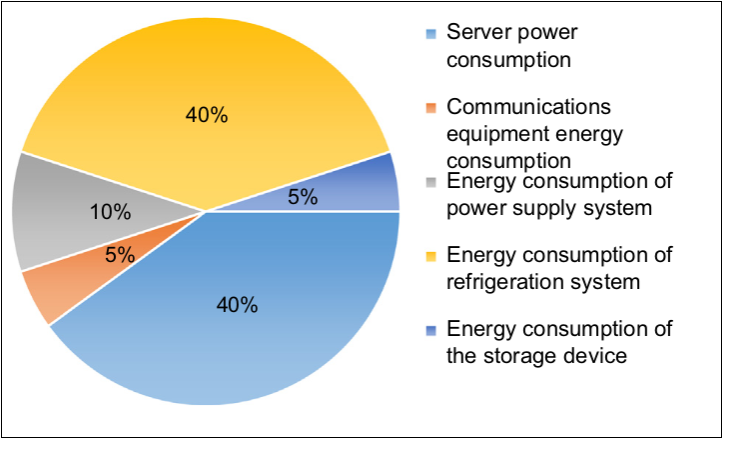
\includegraphics[width=0.5\textwidth]{pics/energyConsumption.png}
	\caption{Energy consumption distribution of data centers \cite{Rong:2016js}}
	\label{fig:consumption}
\end{figure}

Virtualization \cite{Uhlig:2005do} partitions a physical machine's resources (e.g. CPU, memory and disk) into several isolated unit called virtual machines (VMs) where each VM allows an operating system running on them. It rooted back in the 1960s' and was invented to enable isolated software testing. Soon, people realized it can be a way to improve the utilization of hardware resources. Thereafter, a resource management strategy of server consolidation was invented.

Server consolidation \cite{Zhang:2010vo} resolves the low utilization problem by gathering virtual machines (VMs) into a fewer number of physical machines (PMs), so that the resource utilization of PMs are maintained at a high level.  
In the meanwhile, idle servers are turned off to save energy.

\textcolor{Blue}{Difficulties}\\
Despite the usefulness of server consolidation, it is a difficult task. 
Server consolidation is often considered as a global optimization problem 
where its goal is to minimize the energy consumption. 
From mathematical model's point of view, it is often modeled as a bin-packing problem \cite{Mann:2015ua}.
Bin-packing problem is a well-known NP-hard problem meaning it is unlikely to find an optimal solution 
of a large problem. Previous research have studied the problem extensively. 
Because of its NP-hard nature, deterministic methods such as  
Integer Linear Programming \cite{Speitkamp:2010ck} and Mixed
Integer Programming \cite{Wang:2016eh} are unsuitable for a large scale problem 
because of the long computation time.  More research proposed heuristic methods
 to approximate the optimal solution such as 
First Fit Decreasing (FFD) \cite{Panigrahy:2011wk}, Best Fit Decreasing (BFD) \cite{Xu:2010vh}.
In addition, manually designed heuristics are designed to tackle the special requirements such 
as \cite{Li:2009wf, Gupta:2008ul, Jung:2008vb}. Although these greedy-based heuristics can quickly solve the consolidation problem,  As Mann's research \cite{Mann:2015ua} shown, 
server consolidation is a lot more harder than bin-packing problem - because of multi-dimension, many constraints - 
therefore, these greedy-based heuristics can not reach a good approximation and be easy to 
stuck at a local optima.

\textcolor{Blue}{New technology}\\
In addition, virtualization technology has evolved to allow finer granularity resource scheduling.
A recent advent of Container technique \cite{Soltesz:2007cu} has drove the attention of both industrial and academia.
Container is an operating system level of virtualization which means containers share the kernel within a VM and provide isolated environment for applications.
This new concept starts a new service model called Container as a Service (CaaS) \cite{Piraghaj:2015uf} is derived from Platform as a Service (PaaS). 
In comparison with traditional models, CaaS gives the responsibility of application 
deployment and resource allocation to the same hand of Cloud provider.
Hence, Cloud providers have a better control of their resources, however the management difficulty also increases. 
Currently, vast amount of research focus on VM-based server consolidaton can not be directly used on Contained-based model.
This thesis, therefore, aims at providing an end-to-end solution the contained-based server consolidation problem.


% World Energy Outlook 2013 \cite{energyOutlook} estimated world electricity demand for 
% data centers was expected to increase by 66\% over the 2011 to 2035. 
% Beyond that, data centers also have an enormous impact on carbon 
% dioxide emissions \cite{2010arXiv1006.0308B}.


% % A well-accepted measurement: PUE (Power Usage Effectiveness) \cite{Belady:IMLoaM62}
% % a standard measurement for data center energy efficiency which compares the 
% % total power with the power used to power IT equipment (e.g. server, network equipments). 
% A recent survey \cite{Cho:2016kz} shows that the recent development of cooling techniques 
% have reduced its energy consumption and now 
% server consumption has become the dominate energy consumption component.
% Despite improvements in hardwares, various software techniques have been proposed 
% to reduce the energy consumption of servers 
% such as: Server Consolidation and Dynamic Voltage and Frequency Scaling (DVFS) \cite{}.

% Virtualization \cite{Uhlig:2005ub} is the core technology that not only enables 
% the elastic management of Cloud resource but also can be used to improve the utilization and reduce 
% energy consumption.
% It maps a physical machine's system resource - including processors, memory, and 
% other devices - into isolated units called \emph{Virtual Machines (VMs)} which allows 
% multiple operating system to run on. 
% In essence, virtualization add an extra layer of software called 
% \emph{Virtual Machine Monitor (VMM)} or \emph{hypervisors} that can deploy, 
% release and migrate VMs at runtime. 
% Numerous VMMs have been designed for x86 commodity machines such as 
% Xen \cite{Barham:2003vu}, KVM \cite{Kivity:2007wu}, and VMware ESX server \cite{Barham:2003vu}.
 
% \textcolor{Maroon}{A brief introduction of server consolidation}

% It aims at improving the income by guaranteeing \emph{Quality of Service (QoS)}
% \cite{Calheiros:2011ul} of the maximum number of applications that a datacenter can accommodate.

% The server consolidation techniques on the server-level
% have been extensively studied in the past decade \cite{}. 
% However, the recent development of container technology enables a VM-level of consolidation, which 
% has not driven much attention. 
% Container is a lightweight virtualization
% technology which allows an application running in a single container. 
% Multiple containers can be packed in a single virtual machine. 
% Two main advantages make the container popular. 
% First, containers do not need a Virtual Machine Monitor (VMM) but relies on the operating system; 
% it reduces the overhead used on managing the virtual system. 
% Second, the communication \cite{} between containers are much 
% easier (e.g. inter-process communication) than an inter-VM communication. This feature is 
% particularly useful for micro-service-based Web applications where their processes are packed
% into separated containers.
% This new technology has brought new challenges to server consolidation. 
% Traditional algorithms can not be directly applied since there is an extra level
% of virtualization. Affinity and communication aware allocation play an much important role 
% in container-based environment. Therefore, new techniques and algorithms are need to be proposed. 

% Currently, few literatures address the 

% Therefore, this thesis will focus on providing solutions to 
% container-based server consolidation.

% Mainly, there are two types of method: static and dynamic.
% Static methods are often treated as off-line approaches and applied in a periodical manner 
% where a batch of VMs are allocated to a set of servers. 
% They are conducted at a given point of time when
% the overall utilization in a data-center is degraded into a certain level: 
% e.g, a predefined CPU utilization threshold. Because static methods often consider partial or all VMs
% in a datacenter, it is often treated as a global optimization task \cite{}.
% The static method often models the problem as a off-line bin-packing problem and 
% solved with deterministic or heuristic algorithms. The goal is often to find a global optimal solution
% in terms of server utilization and other criteria.
% Dynamic method is an on-line approach. It assumes a scenario when a single server is 
% overloading with multiple VMs, migrate one of the internal VMs out from 
% the host will release the overloading. Dynamic method is used in between 
% two static consolidation processes to ease the overloaded server as well as consolidation.
% As it only moves one VM at a time, it often applies greedy-based heuristic, therefore, hard to 
% reach a global optimization.





% This thesis, therefore, aims at
% providing an end-to-end solution to the container-based server consolidation problem.

% First, aggressive consolidation causes overloading physical resources. 
% It leads to performance degradation since the application cannot obtain enough resources
% the VM promised. It is hard to determine the maximum level of utilization of a physical machine.

\section{Motivation}
\label{sec:motivation}
\bx{This section identifies the research gaps in  resource management of container-based data centers.}
We will discuss the gaps from three placement decision scenarios: application initial placement, periodic optimization, and dynamic placement.

\subsection{Application initial placement}
\bx{Application initial placement deploys applications when data centers receive a number of requests.} The placement can be seen as a static server consolidation problem. To reduce energy, the strategy allocates applications to a minimum number of physical machines (PMs). For VM-based and container-based cloud, the energy models are different.
% The optimization process can be described as: given a number of  PMs represented as resources (e.g CPU cores and RAM etc);  requested applications (wrapped with VMs or container) represented as aforementioned resources; the objective is to allocate these applications into a minimum number of PMs. The decision variable is the location of each application. The basic constraint is that the aggregative resources of hosted VMs cannot exceed the PM's resource capacity.
% The strategies in VM-based cloud and container-based cloud are different. In VM-based cloud, requested applications (wrapped with VMs) are placed into a minimum number of PMs. The problem in VM-based cloud is often modeled as a bin packing problem \cite{Xiong:2014jq}, with VMs represent items and PMs represent bins. The complexity is NP-hard \cite{Hochbaum:1996ts}. 
\bx{In a VM-base Cloud}, the energy model of application initial placement can be seen as a vector bin packing problem \cite{Leinberger:1999fs}, applications (wrapped with VMs) are packed in PMs (detailed discussion is in Section \ref{sec:vector_bin_packing}).

\bx{In contrast, in a container-based Cloud, the energy model can be seen as a bilevel optimization problem \cite{Colson:2007bu} where each level is treated as a bin packing problem.} The lower level optimizes the placement of containers to VMs and the upper level optimizes the placement of VMs to PMs. The advantage the bilevel model is that the interaction of container-VM and VM-PM placement is considered, so that the global optimal can be achieved.

\bx{Two reasons motivate us to solve the application initial placement in container-based Cloud.} 
First, currently, no research has considered the application initial placement as a bilevel optimization problem. Therefore, it needs to propose a new bilevel energy model. A bilevel model - includes energy model, workload model and prices model - represents the relationship between container, VMs, and energy consumption. Current VM-based models cannot be directly applied because container-based model has two levels of placement. In addition, current VM-based models do not consider the overhead of VM hypervisor because for VM-based cloud there is no better ways to avoid the overhead. However, in container-based cloud, the overhead of VMs can be mitigated by reducing the number of VMs. This can be achieved by consolidating containers to fewer VMs. Furthermore, many VM-based models do not consider a balance between CPUs and memories. The balance is crucial \cite{Tomas:2013iv} in improving utilization of PMs, because the balance in a PM increases the probability of being able to allocating a new application.

\bx{Second, bilevel optimization is known to be strongly NP-hard \cite{Sinha:2013tn}.} Even in the simplest case of linear  bilevel programs, where the lower level problem has a unique optimal solution for all the parameters, it is not likely to find a polynomial algorithm that can find the global optimum solution. The proof for the non-existence of a polynomial time algorithm for linear bilevel problems can be found in \cite{Deng:1998fk}. In contrast, evolutionary computation (EC) is a population-based search mechanism which has been proposed to solve bilevel optimization problems \cite{Wang:2008kb, Wang:2011di, Angelo:2013ee}. EC algorithms have shown promising performance bilevel problems. Therefore, we will investigate EC-based approaches on bilevel problem.

% The optimization interact with VMs and containers, therefore, it cannot be optimized separately. An additional constraint is that each container has its OS requirement which makes them cannot be simply packed into homogeneous VMs. 

% \bx{Container-based placement can be seen as a bilevel optimization problem \cite{Colson:2007bu} where each level is bin packing problem.} Because of the problem structure has changed, previous VM-based approaches cannot be directly applied on the problem. In addition, currently, there is no study considers the container-based placement as a bilevel problem. The advantage of considering it as a bilevel problem is that containers and VMs can cooperate to achieve lower energy consumption. However, the \emph{optimization of joint placement of container and VMs} is very difficult because of the nature of bilevel problem.

% The hierarchy of bilevel optimization makes problems non-convex and strongly NP-hard \cite{Vicente:1994ie}.
% The placement problem in the VM context has been studied for years \cite{Xu:2010vh, Gao:2013gg, Ferdaus:2014ep} and it is often modeled as a bin packing problem . This is because VMs and PMs are naturally modeled as items and bins. Furthermore, server consolidation and bin-packing have the same optimization objective: minimize the number of bins/PMs. The complexity of bin-packing problem is NP-hard which is NP-hard \cite{Hochbaum:1996ts} which means it is extreme time-consuming to find its optimal solution when the number of decision variables is large. However, most research focus on VM-based server consolidation and these methods cannot be directly applied on container-based consolidation because of the different structure.

% \bx{Only few research focus on container-based server consolidation problem. One of research is from Piraghaj and et al \cite{Piraghaj:2015uf}.} They propose a simple heuristics on two-step allocation, thus, did not consider the interaction between two levels (see detailed discussion in Section \ref{container-based-placement}). 
% In addition, their resource allocation system completely relies on dynamic placement without using static methods. Although their system can execute allocation fast, the energy efficiency cannot be guaranteed. 
% Another research \cite{Mann:2016hx} is the earliest study which realizes two-level of placement should be considered together because they are interact with each other. They apply a fixed VM placement algorithm and considering a series of VM selection algorithms. The results also proves that the interaction between two placement cannot be ignored. 


\subsection{Periodic optimization}



% For the lower level of allocation, the objective is to maximize the utilization of resources (e.g a balanced utilization among several resources), while the upper level objective is to minimize the number of PMs. 
\bx{After initial placement, periodic optimization is a routine process that takes existing applications' placement, re-placing them to PMs to optimize the energy consumption.} A technology called live migration can be used to re-place the applications' placement from one PM to another. Live migrations are very expensive since they consume network bandwidth and use the resources on both host PM and targeted PM. Therefore, periodic optimization is a multi-objective task which considers minimizing migration of applications and minimizing the overall energy consumption. Resolving the bi-level multi-objective problem will lead to a high utilization of PMs but it is very challenging.

\bx{Two reasons motivate us to explore solutions for periodic optimization in a container-based cloud}. 
\textbf{First}, no research has considered the periodic optimization in a container-based cloud as a bilevel multi-objective optimization problem. The multi-objective bilevel problem has two potentially conflicting objectives: reducing the number of migration and minimizing the energy consumption.
\textbf{Second}, not many research have considered the robustness of placement. The robustness of placement means the placement is resilient enough to handle the fluctuate workloads without making too many further adjustments. To achieve robustness of placement, periodic optimization must consider the combination of various workloads and the reserved resources on PMs. Currently, most research simplified workloads as static (remains a constant value throughout its life cycle) \cite{Viswanathan:2012ej, Chen:2011fl,Feller:2011vs} for the sake of simplicity. The placement is easy to affect by fluctuations which leads to higher energy consumption. Therefore, we will consider various types of workload to improve the robustness of placement.
% For example, for periodic workload, the average value within a period of time will be considered. 

% \bx{In our research, we will consider periodic optimization as a multi-objective problem with various types of workload \cite{Fehling:2014tl}.} Specifically, complementary workloads can be combined so that it can potentially reduce the migration in the future. Thus, the applications are consolidated in a more robust way. 

% However, in real life, workloads vary with time. According to Fehling , applications' workload are roughly classified into five categories: static, periodic, once-in-a-life-time, continuously changing, and unpredictable. 

% They cannot be treated as a static value in a server consolidation because Therefore, it increases the cost in the future. 




% Only a few research consider applying different strategies on different workloads \cite{Meng:2010gh}. Their experiments showed promising results, however, they only mapped paired workloads which can be further improved by combining multiple workloads.
\subsection{Dynamic placement}


\bx{Dynamic placement is applied on overloading and underloading scenarios which need an immediate reaction on the placement of an application \cite{Beloglazov:2013ht}.} Overloadding and underloading happened when applications are released from PMs or applications are facing a burst of workload. In overloading scenario, PMs are running out of resources which means the applications' performance degraded. The degradation will bring financial punishment for Cloud providers. In underloading scenario, PMs are running in a low utilization which leads to the waste of energy. At these states, it is ideal that applications inside the PM will be placed to other PMs to quickly resolve the problems.
% Overloading is a scenario that the workloads exceed the capacity of its host PM. Hence, one or more applications will be migrated to other PMs. Underloading is when a PM runs in a low utilization, all the applications inside it will be moved to other PMs, so that the PM can be turned off. The common operation in these two scenarios are the dynamic placement \cite{Xiao:2015ik}. Dynamic placement places one application each time in an on-line manner. 

\bx{Three reasons motivates us to explore solutions for dynamic placement}. 
\textbf{Firstly}, no research has considered dynamic placement in container-based cloud as a bilevel problem. Current approaches \cite{Piraghaj:2016bw} consider two placements as separate tasks. 
\textbf{Secondly}, current VM-based dynamic placement approaches typically applied either simple bin-packing algorithms such as First Fit or manually designed heuristics. Simple bin-packing algorithms may perform poorly because application placement is more complicated than bin-packing \cite{Mann:2015ua}. Therefore, even for the placement of VMs to PM, it is difficult to reach a global optimal solution. \textbf{Thirdly}, manually designed heuristics may not be general (in terms of decision variables and constraints) because they are designed for specific conditions and constraints \cite{Jung:2010dt}, e.g considered the network topology in data centers. We want to develop a hyper-heuristic approach which can automatically generate good heuristics based the knowledge learned from previous placement solutions.

% The hyper-heuristic can learn from previous good solutions as well as the features of various workloads so that the dispatching rules can be applied with any conditions and constraints. 
% on one hand, dynamic placement allocates an application at a time to meet the requirement of fast reaction. On the other hand, it only considers the best placement of the current application using either simple bin-packing algorithms such as First Fit or manually design heuristics. Simple bin-packing algorithms may perform poorly because application placement is more complicated than bin-packing \cite{Mann:2015ua}, while manual designed heuristics may not be general because they are designed for specific conditions and constraints\cite{Jung:2010dt}.
% Mann's research  showed, server consolidation is a lot harder than bin-packing problem because of the multi-dimensional of resources, heterogeneous PMs, migration cost etc. 


In summary, shortcomings of current resource management in container-based cloud increase the energy consumption of a cloud data center. Therefore, our goal is to reduce the energy consumption by overcoming these limitations in each of placement decision scenario.


% \bx{These challenges motivate us to develop a hyper-heuristic approach which can automatically generate heuristics for quickly placing.} 

% In addition, in container-based Cloud, the placement target is on containers and the destination is a suitable VM. However, if no VM can accommodate a container, a new VM must be created, which incurs a second level of deployment.

% \bx{In summary, this thesis aims at improving the energy efficiency in a container-based cloud data center.} The gaps in three resource management processes motivate us to address three issues:
% \begin{itemize}
% 	\item Develop an algorithm for the joint placement of containers and VMs.
% 	\item Develop an algorithm for multi-objective joint placement of containers and VMs with consider various workloads.
% 	\item Develop a hyper-heuristic for dynamic placement.
% \end{itemize}




% The motivation for this thesis mainly includes two parts, in the first part, we illustrate the roots of container-based server consolidation problem. In the second parts, we explain the motivations for the objectives.

% \subsection{Motivation For Container-based Server Consolidation Problem}

% Server consolidation \cite{Zhang:2010vo} resolves the low utilization problem by gathering applications or VMs into a fewer number of physical machines (PMs), so that the resource utilization of PMs are maintained at a high level. In the meanwhile, idle servers are turned off to save energy. Traditional server consolidation is VM-based, in comparison with 
% a server host a single application, it can dramatically improve the resource utilization. 


% \begin{figure}
% 	\centering
% 	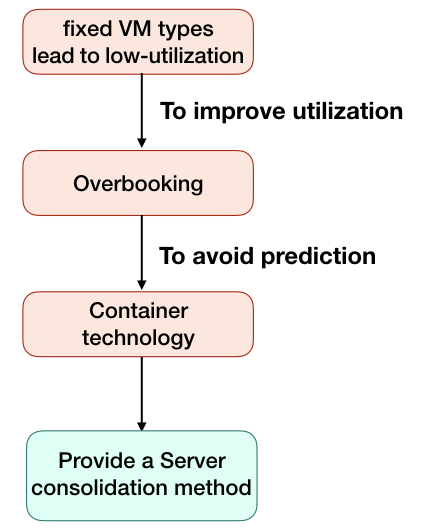
\includegraphics[width=0.3\textwidth]{pics/problem_flow.png}
% 	\caption{The root of container technology}
% 	\label{fig:root}
% \end{figure}
% \begin{enumerate}
% \item Container is a new virtualization technology which provides an operating level of virtualization.
% % Figure \ref{fig:root} illustrates the root of container technology from an energy efficient point of view. 

% In order to solve this problem, overbooking strategy tends to place more VMs than the server's maximum capacity. However, this technique is highly relied on workload prediction on the application running in a VM. Otherwise, servers are easily overloaded. Container technique can improve the utilization by further partitioning VM into resource isolated chunks. Therefore, multiple applications can share the same VM. This technique avoids the prediction of workload as well as improving the utilization. 



% This container technology brings many advantages to current Cloud industry\cite{Felter:2015ki}but it also brings difficulties for server consolidation. Container-based server consolidation adds another level of abstraction which makes it a two-level vector bin-packing problem.
% Therefore, it motivates us to provide \emph{global optimized} resource allocation solution for container-based data centers.

% \end{enumerate}


% \subsection{Motivation For Research objectives}
% Cloud data center has a high dynamic nature where it constrantly receives new requests for resource provisioning and releases old current resources. Therefore, a data center needs different strategies to
% handle different scenarios. 

% \textcolor{Maroon}{In this thesis, we aim at providing a series of approaches to continuously optimize the joint allocation of VMs and containers which involves with three scenarios: application initial placement, periodic consolidation, and dynamic consolidation.} Different stages have distinct goals, therefore, they are considered as separated research questions. 

% \begin{enumerate}
% \item Joint allocation of containers and VMs (application initial placement), \\
% \textcolor{Maroon}{Joint allocation of containers and VMs is the first task when a data center receives new application deployment requests.} At this stage, a set of containers is allocated to a set of VMs and these VMs are allocated to a set of PMs. This task is challenging because the problem is a bilevel optimization where each level is a bin packing problem. Exhaustive search of entire solution space is practically impossible, for the number of possible permutation of solution is huge. Current approaches \cite{Piraghaj:2016bw,Hindman:2011ux} use simple heuristics such as First Fit to solve the problem. These greedy-based heuristics do not consider the complex structure of the problem, therefore, often reach a local optimal solution.

% Only a few research focus on this  problem, Piraghaj \cite{Piraghaj:2016bw} designs a dynamic allocation system. She proposes a two-step procedure. Since, these two-level structure interact each other, separate solution certainly leads to a local optima. Therefore, in this thesis, we will solve the problem simutaneously.
% Most importantly, and therefore can not be solved separately. This is the first research that consider server consolidation has a bi-level optimization problem \cite{Wen:1991kt}. 

% In this objective, we will establish the fundamental concepts in studying this joint allocation of containers and VMs including new problem models: price and power model, new problem constraints, and optimization objectives. The major challenges for this objective is to design representations and several EC approaches to solve this problem. More specifically, in designing the EC approach, new search mechanisms, operators will be designed and new representations will be proposed to fit the problem. 

% This task is challenging, since a representation can highly affect the performance of consolidation \cite{SoteloFigueroa:2013be}. 

% \item Periodic consolidation, \\
% \textcolor{Maroon}{A periodic consolidation is conducted to improve the global energy efficiency in a periodical fashion.} Data center constantly receives new allocations, releasing of old resources. These changing degrades the compact structure of a data center. Therefore, the data center needs a global optimization to improve the overall energy efficiency.

% The challenges are three folds, firstly, similar with initialization problem, the problem has two level of allocations and they interact with each other. Secondly, like VM-based consolidation, Container-based consolidation is considered as a multi-objective problem with minimization of migration cost as well as keeping a good energy efficiency. In bilevel optimization, multi-objective can be defined in either or both level, therefore, it further increases the complexity. Thirdly, consolidation needs to consider different types of workload which may lead to more migrations in the future(\textcolor{Maroon}{NEED MORE EXPLANATION}).

% \item Dynamic consolidation,\\
% Dynamic It takes one container and allocates it to VMs. Since the size of container can be dynamically adjusted, when the an application is under-provision or over-provision, the original container is halted, resized and re-allocated. Hence, there is a need to allocate this new container in real time.

% To solve a dynamic consolidation, heuristics and dispatching rules are often used \cite{Sarin:2011fu, Shi:2011ke, Forsman:2015ca, Beloglazov:2012ji}.  In this scenario, a dispatching rule is considered as a function that determines the priorities of VMs that a container can be placed. However, dynamic placement is much complex than bin-packing problem \cite{Mann:2015ua}. Because of its dynamic nature, human designed heuristics are ill-equipped in approximating solutions when the environment has changed \cite{SoteloFigueroa:2013be}. 

% Hyper-heuristic methods, sepcifically, Genetic Programming (GP) technique \cite{Banzhaf:1998wc} can learn from the best previous allocation and automatically evolves dispatching rules to solve this problem. GP has been applied in generating dispatching rules for bin-packing problem \cite{Burke:2006ei, SoteloFigueroa:2013be} and other scheduling problems \cite{Nguyen:2014eu}. The results have shown promising results.

% There are mainly two challenges, first, it is difficult to identify the related factors that construct the heuristic. Factors or features are the building blocks of heuristics. It is a difficult task because the relationship between a good heuristic and features are not obvious. Second, representations provide different patterns to construct dispatching rules. It is also unclear what representation is the most suitable for the consolidation problem.


% and representations must be proposed to capture the characteristic of the joint allocation. 
% 	and the VMs are allocated to physical machines in the second step. Because of the complexity, previous research
% 	only considers the first step. They map the incoming tasks into predefined categories and based on the characteristic of the categories, the size of new virtual machines' resources are decided. After each tasks have chosen its VM type, they are allocated to virtual machines using a lightweight heursitic algorithm. 
% 	We intend to apply an EC-based approach to solve this problem by proposing a coevolutionary that simuetiously decide the virtual machine type as well as the allocation of VMs.


% \item Large-scale of static server consolidation problem, \\
	% In this case, initialization and periodic consolidation are belonged to this category. 
	% Since Cloud data center typically has hundreds of thousands PMs and more, static server consolidation is always very challenging. Many approaches have been proposed in the literature to resolve the problem. There are mainly two ways, both relied on distributed methods, hierarchical-based \cite{Jung:2010dt, Moens:2011gk} and agent-based management systems \cite{Yazir:2010bk}.
	% The major problem in agent-based systems is that agents rely on heavy communication to maintain a high-level utilization. Therefore, it causes heavy load in the networking. 
	% Hierarchical-based approaches are the predominate methods. In essence, these approaches are centralized methods where all the states of PMs within its region are collected and analyzed. The major disadvantage of hierarchical-based approaches is that it only provides local solutions. In fact, it is infeasible and unnecessary to check all the states of PMs since the search space is too large and most PMs do not need a change. This idea
	% motivates a way to improving the effectiveness is to reduce the number of variables so that the search space is narrowed. In this thesis, we are going to investigate the way to eliminate the redundant information.
% \end{enumerate}



% Traditional Cloud computing offers three services models: Infrastructure as a Service (IaaS), Platform as a Service (PaaS) and Software as a Service (SaaS). Both IaaS and PaaS describe how does a service provider use the cloud resources. The main difference of these two models are  
% IaaS allows service providers to manage the low-level details including the operating system and libraries. While, PaaS provides a higher level of abstraction where users only focus on the application development without caring the underlying operating system and system-level of resources such as CPU cores and memories. However, one drawback of PaaS is that cloud users must make sure their applications are complete compatible with the platform. And in many of the cases, it is not the situation. In order to solve this problem, a container-based virtualization technology starts to reform the Cloud industry. Container as a Service (CaaS) 
% is a new concept but it has been used in industry for many years. Containers provide an operating system-level of isolation environment for applications. It does not need a hypervisor but complete rely on the operating system. 


% This exciting new technology has bring so many advantages for both Cloud users and Cloud providers. From the providers' perspective, In a large system, running VMs means there are probably many same operating systems occupying memories and storages. Lightweight containers share operating system and therefore, there are more rooms for softwares. It increases the capability of Cloud data centers. Furthermore, in terms of resource utilization, it provides much finer granularity operation than a VM-based Cloud model. Containers partition
% a VM into smaller chunks so that with appropriate management, better energy efficiency can be achieved. From the cloud users' perspective, each container provides separated libraries for specific application.  Therefore, it does not contrained by the underlying platform. Like PaaS, Cloud users do not need to concern the scalability of applications. 
% Therefore, CaaS can potentially become one of the main stream in the future Cloud computing industry. 

% Secondly, energy-efficent computing has been the major concern since the begining of computers. Specifially, Cloud computing has become a popular form. Large-scale data centers have been built around the world. A data center can consume huge amount of energies and it needs to improve its energy-efficiency from multiple perspectives. As we discussed in the Introduction, computing servers are one of the major contribution to the energy consumption. 
% And according to observation by \cite{}, the average utilization resource are still very low which causes huge energy wastage. As we mentioned above, the container technolgy provides a better way of managing resources, it has the potential to largly improve the utilization than current VM-based Cloud model because it avoids some of the major drawbacks of VM-based model. 

% Thirdly, because the container technology is relatively new, previous research are mostly focus on IaaS model and so that the server consolidation has based on the VM-level. However,   

% Frist is this new technology of container that can potentially change the landscape of
% Cloud computing. It has so many benefits but also it brings difficulty in managing resources.

% Second, from green computing point of view, we still need to manage resource so that, the 
% data centers consume less energy. And container technolgy actually bring a better chance to
% be more energy-efficient than previous VM based technology.
% Third, it is very difficult to manage this container-based resources because of the problem-nature is too complicated. And existed algorithms can not be directly applied on it.
% Fourth, the evolutioanry computation provides a good framework to handle such difficult problem.

% \textcolor{Blue}{Motivation is what is now lack from the literature.} \\

% The advantage of Platform as a Service (PaaS) has been discovered in the recent years. 
% The disadvantage of tranditional IaaS model has been discovered in the recent years \cite{Mann:2016hx}.
% In IaaS, on one hand, cloud customers need to manage the low-level details ranging from application capacity estimation,
% resource planning and selection and deployment. 
% On the other hand, Cloud providers manage resource provisioning and allocation. 
% Although these two tasks are seemingly different, 


% The container as a Service (CaaS) cloud model has gain increasing attention in the recent years.
% However, the energy efficiency in CaaS cloud environment has not been investigate. 
% Particularly, the virtual machine and container joint consolidation is the core problem.
% Therefore, in this thesis, we will focus on the end-to-end energy-aware server consolidation on container-based
% Cloud. In the meanwhile,  a major research direction of large scale server consolidation is also considered. 
% The end-to-end server consolidation refers to the server consolidation techniques used
% in the different stages throughout the routine Cloud resource management including  initial VM provisioning and placement, dynamic VM placement, and static VM placement:

\section{Research Goals}

\begin{figure}
	\centering
	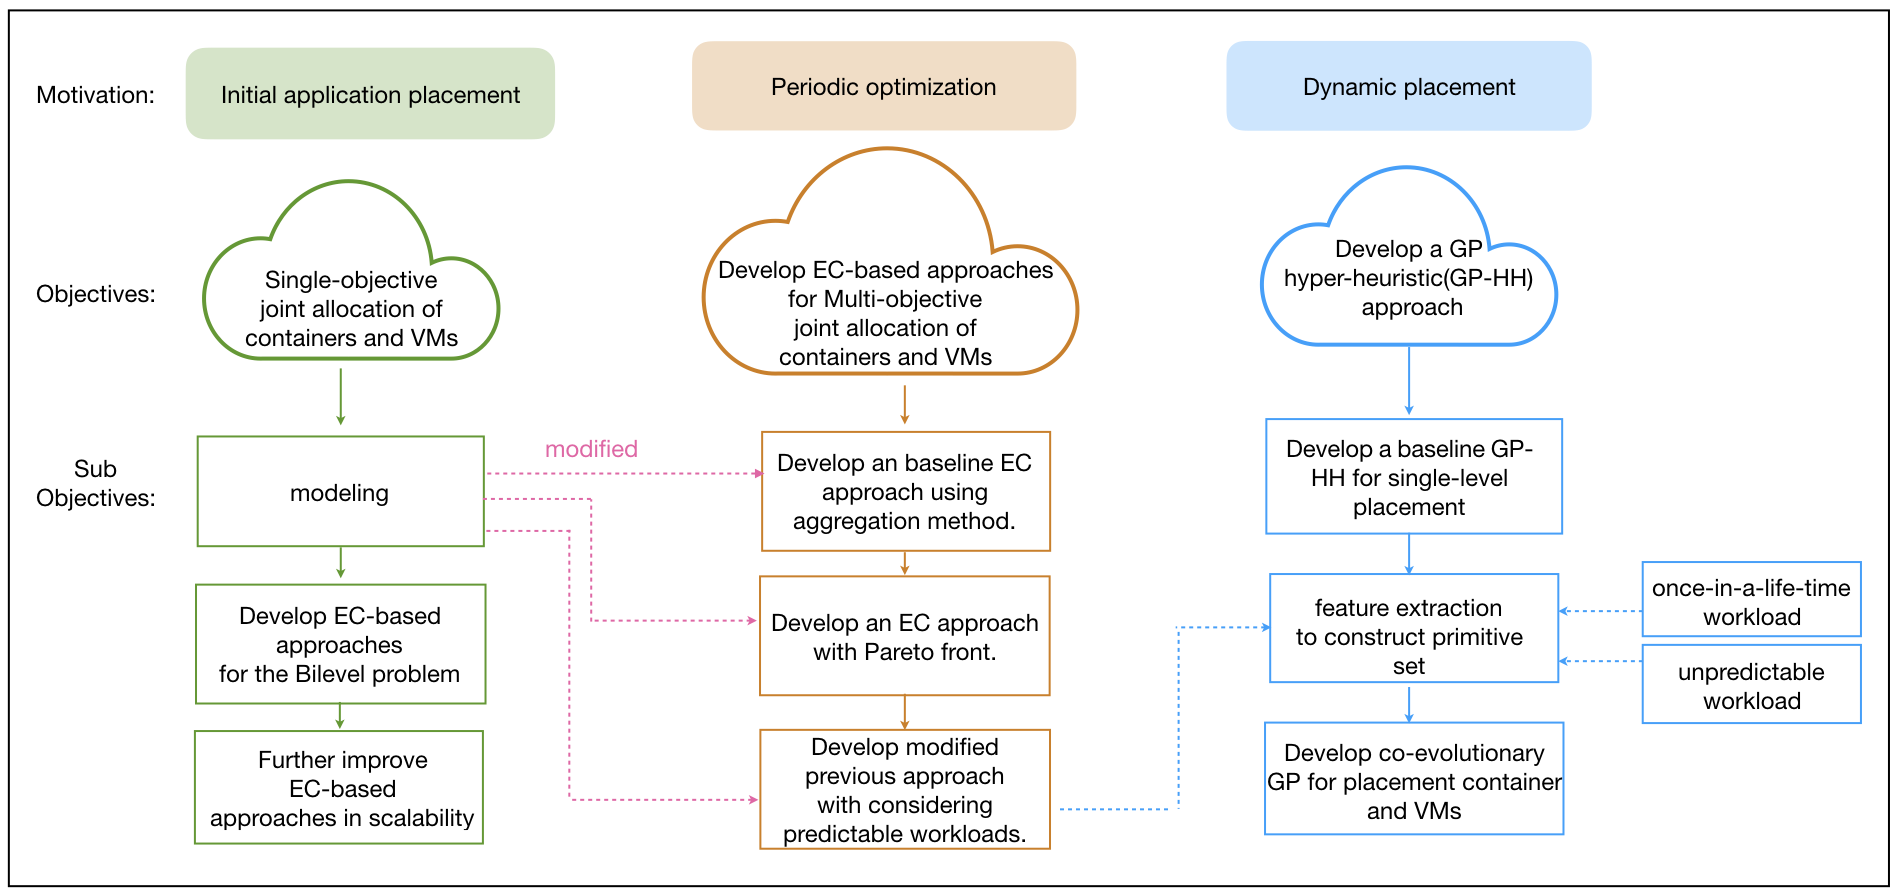
\includegraphics[width=\textwidth]{pics/thesisPlan.png}
	\caption{Relationship between objectives}
	\label{fig:objectives}
\end{figure}
\bx{The overall goal of this research is to optimize energy consumption of a container-based Cloud data center using EC-based approaches for three placement decision scenarios:} initial placement of application, periodic placement of application, and dynamic placement of application. The specific research objectives of this work can be itemized as follows.
% In this thesis, we aims at providing a series of approaches to continuously optimize the a joint allocation of VMs and containers that considers three consolidation scenarios: Initialization, global consolidation, Dynamic consolidation. In addition, the static allocation normally involves with large amount of variables which is particular difficult to optimize. We are also going to propose a method to solve this problem.  These approaches combine element of AI planning, to ensure the objectives and constraint fulfillment, and of Evolutionary Computation, to evolve a population of near-optimal solutions. The research aims at determining a flexible way in creation of solutions to solve server consolidation problems. As discussed in the previous section, the research goal can be achieved in the following objectives and sub-objectives.

\subsection{Objective One: Develop EC-based approaches for the single objective joint placement of containers and VMs for initial placement of application}
\label{sec:obj1}

\bx{The goal of objective one is to minimize energy consumption in initial placement of application at container-based cloud.} We set three sub objectives to achieve this goal. The first sub objective is to propose a new bilevel energy model for the joint placement of containers and VMs in PMs. The second sub objective is to develop an EC-based optimization algorithm to solve the joint placement of containers and VMs. The third sub objective improves scalability of the proposed EC-based optimization algorithm. Note that, we will use ``the bilevel model/problem'' to replace ``the joint placement of containers and VMs model/problem'' in the following content. 
% \textcolor{Maroon}{Currently, most research on container consolidation do not consider the two-level of allocation problem.} Unlike previous VM-based service consolidation, 
% most research focus on VM-based server consolidation technique. They often modeled the VM allocation problem as a vector bin-packing problem \cite{Zhang:2016cx}. 
% Container adds an extra layer of abstraction on top of VM. The placement problem has become a two-step procedure, in the first step, containers are packed into VMs and then VMs are consolidated into physical machines. These two steps are inter-related to each other. Previous research \cite{Piraghaj:2015uf} solve this problem in separated steps where the first step allocates containers to VMs and the second step allocates VMs to PMs with simple bin-packing heuristics. According to Mann's \cite{Mann:2016hx} observation, these two allocations should be conducted simultaneously to reach a near-optima solution, which essentially minimizes the energy consumption.

\begin{enumerate}
	\item Develop a new bilevel energy model to represent the relationship between six factors and energy consumption. The five factors involves locations of container, types of VM, locations of VM, overheads of VM, and the balance between memory and CPU. We need to consider the interaction between these factors.
	% \textcolor{Maroon}{This problem can be considered as a bilevel problem \cite{} the lower-level optimization: allocate containers to VMs and the upper-level: allocate VMs to PMs.} 
	% \textcolor{Maroon}{Since the existing models for container-based consolidation are based on VM-based model which incurs two problems.}
	% First problem is that they did not consider the interaction between two levels of allocation.
	% Second problem is that they did not consider balancing the residual resources (e.g between CPU and memory). 
	% \bx{The goal of the first sub objective is to propose a bilevel model for the joint placement of container and VM.} 

	\bx{The major challenge of this sub-objective is that the bilevel energy model is more complicated than a single-level energy model.}
	\textbf{First}, in VM-based model, the only factor is the locations of VMs in PMs. In contrast, in container-based model,  the energy model involves with four more variables such as the locations of containers in VMs, types of VM, overheads of VM, and the balance between memory and CPU. Specifically, the factor of locations of container decides the placement of applications. We consider types of VM because the containers may have constraints on the types of VM. Overheads of VM should also be considered because appropriate placement containers can minimize the overheads of VM. The balance of CPU and memory has an impact on the energy consumption \cite{Mishra:2011bz}. The better balance will lead to a higher probability of being able to allocate more applications.

	Three challenges are listed as follows. \textbf{First}, the bilevel energy model is more complicated than a single-level energy model. The relationship among variables of the bilevel energy model has not been explored. In the VM-based energy model, the only variable is the location of VMs in PMs. In contrast,  container-based energy model has more variables such as the location of container, type of VM and the location of VM. \textbf{Second}, the balance of CPU and memory has an impact on the energy consumption  The more balance between CPU and memory in a PM, the higher probability of being able to allocate more applications. However, in container-based cloud, defining this balance is not straightforward because an additional variable of VM type has not been considered in previous study. \textbf{Third}, the overheads of VMs has not been considered in VM-based model because there is no better way to avoid the overheads. However, in container-based cloud, the overhead of VM can be mitigated by reducing the number of VMs. Therefore, adding the overhead of VM to the container-based energy model is necessary. 

	% The first issue is that it is still unclear that which energy function is the best to capture the relationship between container and VM so that the overall energy is low. Specifically, the objective for the lower level - placing container to VM, is still unclear. This is because the minimum number of VM does not necessary lead to the minimum number PMs; the types of VM also play an important role.
	% The second issue is that previous VM-based research do not consider the overhead of VM. However, the overhead of VMs is a major source of resource wastage (addressed in Section \ref{sec:comparison_container_vm}). Therefore, how to represent the impact of VMs remains unsolved.
	% The third issue is related to a VM-based research,  Mishra \cite{Mishra:2011bz} discovered that when multiple resources are considered in the model, the balance between resources has a heavy impact on the optimization results. Therefore, in the bilevel model, the balance of resources should also be considered.

	In order to establish a bilevel energy model, we will follow three steps. First, we will review a number of literature discussing the overheads of VMs. One possible way is to represent the overheads of VMs as the utilization of resources. The relationship between the utilization of resources and the types of VM needs to be investigated.  Second, we will review literature about how to represent the balance between CPU and memory. For the bilevel energy model, both VM and PM requires a balance between CPU and memory so that the utilization can be maximized in both levels.

	the VM-based energy model to establish the variables and constraints. The relationship between VM, PM and energy consumption can be found in literature. However, the relationship between container and VM is not straightforward because of the overhead of VM and 

	Each level of the problem will be formulated to a multi-dimensional vector bin packing problem. 
	We will start from the simplest case - single dimension of resource - to more general multi-dimensional resources model by reviewing a number of VM-based approaches. Specifically, we focus on their variables, constraints and objective function. Objective function is mainly related to energy consumption. Hence, energy model is another major issue to study. In addition, in the multi-dimensional resource model, we will address the balance of CPU and memory problem by investigating several resource wastage models \cite{Ferdaus:2014ep, Xu:2010vh, Gao:2013gg}. In this objective, we consider the static workload of applications, this is because the initial resource demand is often provided by the Cloud users.


	% The novel contribution of this sub-objective is 


	\item Propose a new EC based bilevel optimization approach to solve the initial placement of application.\\
	\bx{Based on the proposed bilevel model, the goal of this sub-objective is to develop an approach for the bilevel optimization problem using nested Evolutionary algorithms \cite{Sinha:2017et}.}

	\bx{Three challenges need to be solved. First one is to understand the interaction between bilevel's placement.} In the bilevel problem, placing containers into a minimum number of VMs does not necessary lead to the minimum energy consumption. Therefore, it is still unclear that relation among the selection type of VM, placement of container and placement of VM will affect the energy consumption. Second challenge is how to design the search operators and representation. Currently two types of representation: direct and indirect representation can be considered. However, it is unclear that which one is more suitable for the nature of the bilevel problem. Third, bilevel optimization is strongly NP-hard \cite{Mathieu:2011dw}, the solution space can be non-linearity, discreteness, no-differentiability, and non-convexity. Therefore, it is extremely difficult to design a proper search mechanism to find near optimal solutions.

	In order to discover the relation among the selection type of VM, placement of container and placement of VM, we will first use one type of VMs and one type of container. By controlling these variables, the effect of different types of VMs and containers will be eliminated. Therefore, the relationship between bilevel placement would be clear. We will gradually add up variables and constraints. For the representation of bilevel problem, we will develop direct binary representation \cite{Xu:2010vh}, and indirect continuous probability representation \cite{Xiong:2014jq}. Genetic operators are also designed along with the proposed representation.
	Current nested methods have been used in solving bilevel problem, however, there is no research focus on bilevel bin-packing problem. We will investigate several approaches such as Nested Particle Swarm Optimization \cite{Li:2006br}, Differential evolution (DE) based approach \cite{Angelo:2013ee, Zhu:2006in} and Co-evolutionary approach \cite{Legillon:2012dd}.

	\item Investigate methods to improve the scalability of the EC-based bilevel optimization approach.

	\bx{Based on proposed EC-based approach, the goal of this sub-objective is to improve scalability of the approach.} Although nested approaches have been reported effective, they are very time consuming \cite{Sinha:2017et}. Therefore, this sub objective intends to explore other directions to improve the execution time. 

	\bx{Three approaches can be potentially used in improving the scalability.} The first one is single-level reduction \cite{Sinha:2017et}, which reduces the bilevel problem into a single dimensional problem. Containers can be categorized into VMs which is then placed into PMs. The combination of container must be based on the knowledge of two-level placement interaction which we discover in the previous objective. Clustering approaches such as K-means \cite{Xie:2011fj} or decision tree can be useful in categorizing containers. Then, complementary containers can be grouped to reduce the variables of placement. The challenge is to identify the features of static workload so that different workloads can be combined to fill a VM. Another way is use reinforcement learning to learn the pattern of energy-efficient combination of containers. 
	The second approach is using a divide and conquer method to split the large number of containers into smaller chunks. The main challenge is that how to split the problem is unknown. Randomly dividing is very likely lead to a sub-optimal solution.
	The third approach is combine heuristics into the EC algorithm, for example, develop a representation which is embedded with a simple heuristic (e.g First Fit). The heuristic is expected to reduce the search space so that the EC algorithm can find solution more efficiently. However, design a heuristic which embedded inside an EC algorithm is extreme difficult since evaluation of heuristic is indirect. 

	% \item Third, although nested approaches have been reported effective, they are often very time consuming. Therefore, our third sub-objective will focus on developing more efficient algorithms. There are several possible directions to be explored such as metamodeling-based methods \cite{Wang:2007em} and single-level reduction. 
		% \emph{New operators and searching mechanisms}\\
		% In order to utilize Evolutionary Computation (EC) to solve this problem, we are going to develop searching mechanisms according to the nature of problem as well as the selected representation. In order to achieve this goal, we will design several new operators. In order to evaluate the quality of these components, we will perform analytical analysis on the result.
\end{enumerate}
\subsection{Objective Two: Develop EC-based approaches for the multi-objective joint allocation problem for periodic placement of application}
The goal is to develop multi-objective EC-base approaches for container-based cloud in periodic placement of application with considering various types of workload to reduce the overall energy consumption.

% As previously (see Section  \ref{sec:motivation}) mentioned, the task is multi-objective: minimizing the number of migration and minimizing the overall energy consumption. This two objectives are conflicting since intensive optimization may incur a large number migration. The first challenge is how to solve the multi-objective bi-level optimization problem. In addition, we consider propose a robust periodic placement of application which means the placement of applications does not affect much from the variant workloads. Therefore, we divide workloads into five categories according to Fehling \cite{Fehling:2014tl}: static, periodic, once-in-a-life-time, continuously changing, and unpredictable. Among five types of workloads, two of them:  once-in-a-life-time and unpredictable workloads are unsuitable for static placement, since their behavior are hard to foresee and plan, hence, they are normally solved by dynamic approaches which will be addressed in our third objective.  For static, periodic, and continuously changing workload, we are going to design specific solutions. We also use three questions to guide our objective.
% The robustness of a data center is particularly important. 
% The robustness measures the stableness of result of consolidation.
% Furthermore, we will investigate proactive approaches - considering future allocation.
% In order to measure the degree of robustness, we need to design a robustness measure. The second sub-objective is to design static consolidation algorithm with considering its previous immediate result. The third objective extends the second objective to a more general case, considering both previous immediate and next allocation. The evaluation of algorithm is based on analytical analysis of fitness functions and robustness measure. 

\begin{enumerate}
	\item Modify the proposed model to adapt to the multi-objective problem with various types of workload. \\
	\bx{The goal of this sub-objective is to modify previous proposed bilevel model so that it adapts to the multi-objective problem.}

	\bx{There are mainly two challenges, the first one is to add an migration model to the existing model, and the second is to adapt the model to various types of workload.} The migration model is distinct with VM-based model. Because both container and VM can be migrated, it is unclear that migration model should be added to both layer or just one. One possible solution is to represent all VM migration with container migration. It may reduce the complexity. In addition, majority traditional migration models only consider the migration number without including the size of the applications which is unrealistic. Because the size will affect the overhead on the networking. 
	The second challenge is to adapt the model to various types of workload. Previously, we simply the problem as applications can be represented as static workloads. In this sub objective, we consider three types of predictable types of workload: static, linear continuous changing and periodic workload. These workloads may be represented as a function of time. Other models may also be changed accordingly.

	% We will further develop an EC-based multi-objective algorithm with aggregation approach to test the model. The aggregation approach turns a multi-objective problem into a single-objective problem by combining objectives into a single one. Therefore, we may use previous developed algorithm to solve periodic placement of application problem. We will use static workload to test the model. 

	\item Propose an EC-based multi-objective algorithm for periodic placement of application with Pareto front approach.\\
	\bx{The goal of this sub-objective is to develop an EC-based approach to solve the multi-objective joint allocation problem with Pareto front approach.} 

	The major challenge in this sub-objective is to design genetic operators so that the proposed algorithm can steer the search close to the correct Pareto front. The aggregation approach proposed in previous sub objective has some defects such as it cannot find the non-convex solution. A Pareto front approach is able to find a set of trade-off between objectives, therefore, we decide to explore this direction. Currently only a few research \cite{Yin:2000bt, Deb:2009jh,Deb:2010in} focus on bilevel optimization problem. This will be the first time that bilevel optimization with Pareto front approach is applied on a bilevel bin packing problem.
	% However, most of them are designed for continuous problems. Therefore, new representations and operators need to be considered for discrete problem. 

	% The assumptions for this objective, we will start from one dimensional of resource: CPU utilization. We will consider the static workload in this sub objective because they are common and easy to start with.  We can utilize the representation and problem models from previous objective. However, we need to propose new genetic operators to adapt the multi-objective problem.

	% like the case in single objective problem, we need to develop new representations, genetic operators.
	\item Propose an EC-based multi-objective algorithm for periodic placement of application considering various types of predictable workload. \\
	\bx{The goal of this sub objective is to propose an approach for three predictable workloads \cite{Fehling:2014tl}: static, linear continuously changing, and periodic.} The major challenge for this objective is that the change of problem model from static to changing workload may lead to a different representation. In order to achieve using a uniform representation for various workload, we are going to explore various workload. Accordingly, new search mechanisms must be proposed to adapt to the representation.
	% Factor analysis such Principle Component Analysis \cite{Wold:1987wx} can be employed in developing new measure. Meanwhile, the representation used in static workload might not work, therefore, new representation, genetic operators need to be developed. 

	% Proactive consolidation \cite{Farahnakian:2015vj, Tan:2011jd} has driven a lot of attention in recent years. They mainly focus on making prediction of the workloads using a regression approach such as linear regression, multi-linear regression, and K-means regression. However, most of their consolidation methods are simple heuristics. In our approach, we seek to propose a combined technique.

	% \item Second, we will design a robustness measure. Previous studies only use simple measurement which counts the migration number between two static consolidation. This measurement aims at minimizing the number of migration between two  static placement processes. It may cause more migration in the next consolidation. Therefore, it needs a time-aware measure of the robustness of system. Therefore, in this objective, the first sub-problem we are going to solve is to propose a robustness measure. Currently, only a few research propose robustness aware server consolidation techniques \cite{Takouna:2014fa, Grimes:2016ia} have been proposed. They are either static threshold or probability-based threshold to measure the robustness of PMs. We will investigate an adaptive measure based on the historical data and current status.
	

	
	% \item \emph{Design a }\\

		% We will generalize the previous sub-objective to a more general one: design a time-aware allocation method which takes previous and next allocation into consider.
	\end{enumerate}

\subsection{Objective Three: Develop a hyper-heuristic single-objective Cooperative Genetic Programming (GP) approach for automatically generating dispatching rules for dynamic placement of application.}

\bx{The goal for this objective is to develop a cooperative GP-based hyper-heuristic algorithm so that the generated dispatching rules can achieve both fast placement and global optimization with various workloads.}

% Previously, dynamic consolidation methods,including both VM-based and container-based, are mostly based on bin-packing algorithm such as First Fit Descending and human designed heuristics. As Mann's research \cite{Mann:2015ua} shown, server consolidation is more harder than bin-packing problem because of multi-dimensional of resources and many constraints. Therefore, general bin-packing algorithms do not perform well with many constraints and specific designed heuristics only perform well in very narrow scope. Genetic programming has been used in automatically generating dispatching rules in many areas such as job shop scheduling \cite{Nguyen:2014eu}. GP also has been successfully applied in bin-packing problems \cite{Burke:2006ei}. Therefore, we will investigate GP approaches for solving the dynamic consolidation problem. We will start from considering one-level of problem: migrate one VM each time to a PM. 

% Therefore, in this objective, we will use GP to automatically generate heuristics or dispatching rules.

\begin{enumerate}

	\item Develop a GP-based hyper-heuristic (GP-HH) algorithm for the placement of container to VM. \\
	\bx{In order to develop a cooperative GP-based hyper-heuristic to the bilevel problem, it is necessary to develop a GP-HH for the single level of the problem. Therefore, the goal of this sub-objective is to develop a GP-HH algorithm for placing containers to VMs.} This task is none trivial since no GP-HH has been dynamic placement of application problem. Therefore, we may start from considering the features such as the status of VMs (e.g resource utilization), features of workloads (e.g resource requirement) that will affect the placement decision. We will construct primitive set with the selected features. Other unsolved issues are the functional set and search mechanism. We will use the functional set by using the general operators. The original genetic programming will be used as the search mechanism. 

	To train the GP-based hyper-heuristic, we will use the solutions in the first objective as the model solution. 

	In order to evaluate the automatically generated heuristics. We will use a widely used simulator called CloudSim \cite{2009LNCS.5931...24B}. Since our proposed algorithm is focus on one level of placement, it is equivalent to the VM-based placement problem. We will compare our heuristic to a highly cited work \cite{Beloglazov:2012ji} from Beloglazov who propose a Best Fit Decreasing heuristic for the energy consumption problem.

	\item Conduct feature extraction on the predictable workloads and unpredictable workloads. \\
	\bx{The goal of this sub-objective is to construct a GP primitive set by applying feature extraction on various types of application workload.} In previous sub-objective, we develop a baseline GP-HH on static workload. In order to develop a general GP-HH that can handle all kinds of workloads, we will extract features from predictable workloads such as linear continuous changing workloads, periodic workloads, and from unpredictable workloads: once-in-a-lifetime workloads. 

	The first challenge is to find suitable representation for workloads. Currently, representation time-series are classified into three categories: temporal, spectral and others. It is still unclear which pattern extraction technique and representation that is best for workload data. The second challenge the high dimensionality of dataset which requires a dimensionality reduction technique to reduce the number of data point. Some possible techniques are sampling, extrema extraction.

	We will test the extracted features by applying classification on the training and test set. The final features will be used in the primitive set.

	% types including static, continuously changing, and periodic workloads, and two other workload types: once-in-a-life-time, unpredictable workloads. Based on these features, 
	% \textcolor{Blue}{More...}
	% \item Investigate the possible functional operators. 

	% \bx{The goal of this sub-objective is to construct a GP functional set.}
	% \textcolor{blue}{More will come.}

	\item Develop a Cooperative GP-HH approach to evolve dispatching rules for placing container and VMs. \\
	\bx{The goal of this sub-objective is to develop a cooperative GP approach to evolve dispatching rules.} In the baseline approach, we develop a GP-HH approach for single-level of placement. However, there is a case that no current VM is suitable for a container to place in; a new VM is needed to place at this moment. This case incurs a second level of placement. 

	Therefore, to construct a complete placement dispatching rule, we will develop a cooperative GP-HH approach to solve the two-level of placement problem. We may reuse the single-level GP-HH in both level or develop a new GP-HH in the VMs to PMs level.  

	% This sub-objective explores suitable representations for GP to construct useful dispatching rules. It also proposes new genetic operators as well as search mechanisms. \textcolor{blue}{More will come.}

	\end{enumerate}

% \subsection{Objective Four (Optional) Large-scale Static Consolidation Problem}
% Propose a preprocessing method to eliminate redundant variables 
% Current static consolidation takes all servers into consider which will lead to a scalability problem. In this objective, we will investigate two branches of methods, first one categorizes a number of containers into fewer groups so that the granularity decreases \cite{Piraghaj:2015uf}. Second method categorizes PMs so that only a small number of PMs are considered. This approach will dramatically reduce the search space. The potential approaches that can be applied in this task are various clustering methods.

	% The 
	% initial placement can be considered as a two-level of multi-dimensional bin-packing problem with multi-objectives. 
	% \item First, from the perspective of \emph{Cloud resource allocation model}, 
	% 	traditional Infrastructure as a Service (IaaS) resource allocation model 
	% 	considers service allocation and VM placement as separated responsibility.
	% 	Cloud users or brokers need to concern about the resource mapping and VM selection and 
	% 	Cloud providers take care of the VM placement. 
	% 	However, as Cloud users tend to over-provision in order to satisfy the QoS, they often book more
	% 	resources than their need. This is the major reason for the low utilization in 
	% 	Cloud computing \cite{Vogels:2008bg}. This problem cannot be 
	% 	resolved solely from the Cloud providers' perspective but to change the current resource allocation model. In the new resource allocation model, the responsibility of service allocation and VM placement are in the same hand of the Cloud provider.
	% 	Thereafter, Cloud providers have the full control of resource management. 
	% 	However, this process makes the VM initial placement a more complicated problem. Currently, only few researchers \cite{} have noticed this problem and propose initial work to address this problem.
	% \item Dynamic server consolidation is the process that the resource management continuously detects the server runtime status and if one of the server is overloaded. Then,
	% one of the VM or container running inside the server will be migrated to other machine 
	% so that the applications do not suffer from a performance degradation. In a container-based
	% environment, there are three questions to be answered. \emph{When to migrate ?} refers to determine the time point that a physical server is overloaded. \emph{Which container to migrate?} refers to determine
	% which container need to be migrated so that it optimize the global energy consumption.
	% \emph{Where to migrate?} refers to determine which VM and host that a container is migrated to.  
	% Specifically, in the second question, the main idea in the literature is still simple heuristics and random selection. Therefore, we are going to investigate using a genetic programming technique to learn to choose the best. In the 
	% third question, literature also rely on simple bin-packing heuristics which do not consider the impact of environment. Therefore, we are going to propose an idea which uses the features of workload, to decide which VM
	% is the best choice.

	% \item Static server consolidation is the process that a batch of VM and container joint is
	% consolidated in order to achieve an low energy consumption status. This stage is often
	% applied when the overall energy consumption is reached a predefine threshold. The static
	% server consolidation can globally optimize the energy consumption of the data center.
	% The process is similar with the initialization stage but with different objectives and constraints.

	% \item 

	% \item Second, container as a service has become an important trend in the 		Cloud computing industry and being support by many Cloud providers 	such as Amazon, Azure and many 
	% 	open-source projects. Both Cloud users and providers 
	% 	are beneficial to its lightweight. It provides a finer granularity resource management
	% 	for Cloud providers. From Ref \cite{}, we observed that VM-level consolidation could further improve the utilization of resource as well as the footprint from traditional hypervisors. 
	% 	However, there is not much container consolidation methods were discussed in the literature. 
	% 	New models and consolidation methods need to be proposed to solve the problem. Moreover, similar to
	% % 	VM placement, container placement is also an multi-objective which need to be addressed.

	% \item Third, the joint VM and container poses another level of consolidation problem. Ref \cite{} states, 
	% 	one of the reasons that container consolidation has high SLA violations is because the 
	% 	higher migration rate of containers. Therefore, designing algorithms that dynamically select between VM and container migration based on application SLA requirement as well as the impact on energy consumption is the major concern of the joint allocation. This can be treated as a dynamic task. 

	% \item Fourth, a common problem that faced by both traditional VM-based and the recent container-based data 	center is the affinity aware resource allocation problem. 
	% 	Modern Cloud-native applications normally have more than one copy of its implementation called replica in order to resolve the stateless as well as load balancing problem. Hence, they must be allocated into different servers to maintain its reliability. Similarly, the backup of databases has the same issue. In the CaaS scenario, more constraints appear such as operating system aware allocation which means, 
	% 	certain container can only be allocated in a specific operating system \cite{}. 
	% 	The affinity-aware allocation has been discussed in the literature, 
	% 	however, they can only be applied in the VM-based data center.   
	% \item Fifth, a resource-utilization aware co-location scheme can be helpful in order to resolve the 
	% 	resource competition problem. The study is about the behavior of the applications deployed
	% 	in the same physical machine. The previous research assumes that the applications' behavior
	% 	is a priori \cite{}, however, applications' behavior can be changed over time. It is important to allocate
	% 	the compatible applications in the same physical machine so that the physical machine reaches a 
	% 	stable status.

	% \item Sixth, large scale of server consolidation has always been a challenge in a Cloud data center. 
	% 	Especially, typical number of servers in a data center is at the million-level. Many approaches 
	% 	have been proposed in the literature to resolve the problem. 
	% 	There are mainly two ways, both rely on distributed methods, 
	% 	hierarchical-based \cite{} and agent-based management systems \cite{}.
	% 	The major problem in agent-based systems is that agents rely on heavy communication to maintain a high-level utilization. Therefore, it causes heavy load in the networking. Hierarchical-based approaches are the predominate methods. Hierarchical-based methods, in essence, are centralized systems where all the states of machines are collected and analyzed. One of way to improving the effectiveness of centralized system is to reduce the size of variables without losing too much of the consolidation performance. The main idea is to eliminating the high-utilized servers so that it reduces the dimensionality. 
% \end{enumerate}
\section{Published Papers}

During the initial stage of this research, some investigation 
was carried out on the model of container-based server consolidation \cite{Tan:2017tz}. 

\begin{enumerate}
	\item Tan, B., Ma, H., Mei, Y. and Zhang, M., ``A NSGA-II-based Approach for Web Service Resource Allocation On Cloud''. \textit{
	Proceedings of 2017 IEEE Congress on Evolutioanry Computation (CEC2017). } Donostia, Spain. 5-8 June, 2017.pp. 



\end{enumerate}


\section{Organisation of Proposal}
The remainder of the proposal is organised as follows: Chapter \ref{} provides a fundamental
definition of the Container-based server consolidation problem and performs a literature review covering a range of works in this field; Chapter \ref{} discusses the preliminary work carried out to
explore the techniques and EC-based techniques for the initialization problem; Chapter \ref{} presents a plan
detailing this project’s intended contributions, a project timeline, and a thesis outline.





% \subsection*{Limitation of Current CaaS Server Consolidation}
% We identify the limitation of state-of-the-art server consolidation approaches 
% in terms of two phases \cite{Varasteh:2015fu} and computing system design.
% Phase 1 - Problem definition including objective functions and constraints; 
% Phase 2 - The techniques to solve the optimization problems. 
% From the computing system design point of view, we identify a cross-layer collaborative 
% technique and a VM multiplexing technique which can potentially improve the utilization of 
% computation resources.

% \subsubsection*{Limitation in the IaaS model}
% Infrastructure as a Service is one of the three basic 
% service models (others are SaaS and PaaS) in Cloud computing. Different from other two service 
% models, IaaS allows Cloud customers to manage the low-level details of 
% virtual machine sizes, security settings and network regions. 
% From the perspective of resource management, IaaS separates 
% the concern of customers' task allocation and VM placement.
% Cloud customers or brokers estimate the computational resources they need and map them into
% a set of virtual machines. Once the task allocation is done, 
% Cloud resource management system will find a set of servers and provision the required VM
% on them. 

% However, this separated responsibility has become of a major reason for the low utilization in Cloud
% data centers. Cloud customers and brokers tend to over-estimate the resource they need in order
% to maintain its QoS in the peak service time. In fact, the peak time only accounts for a small portion
% of the overall service period. 
% Although modern virtualization technology allows overbooking strategies, Cloud providers also
% need to keep monitoring the overbooked servers to avoid overload. This surely increases the 
% overhead of management.

% One of the approach to improve the resource utilization is to put 
% the responsibility of task allocation and VM consolidation in the same hand of Cloud providers,
% thereafter, Cloud provider can estimate and dynamically adjust the resource assigned to a task.
% In addition, VM multiplexing can also be used in improving the utilization.
% Mann's research \cite{} gives an example which shows a scenario that simultaneously decide the 
% task allocation and VM placement can reduce one third of the energy consumption.

% \begin{figure}
% 	\centering
% 	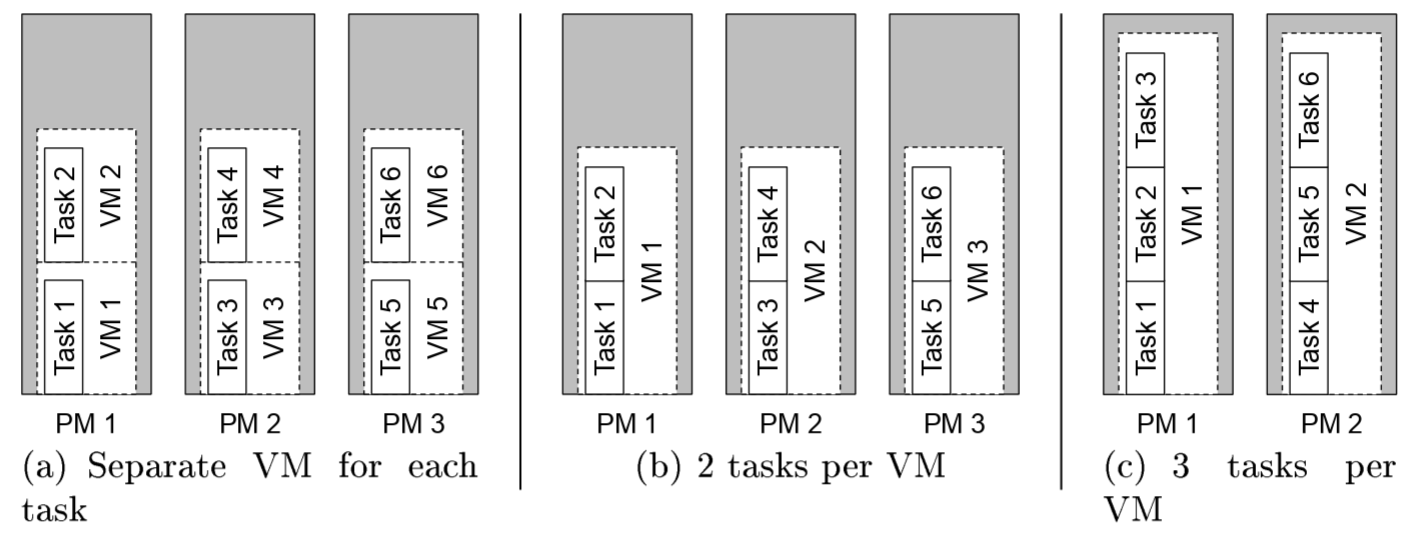
\includegraphics[width=0.8\textwidth]{example.png}
% 	\caption{An example shows VM multiplexing can reduce 33\% of energy consumption \cite{}}
% 	\label{fig:example}
% \end{figure}

% Another limitation of IaaS model is that it only provides limited types of VM with fixed amount resources (including CPU, memory, etc). When a customer chooses VM type, they are forced to
% choose a VM type with the enough resource of a critical resource (e.g. CPU), therefore, other resources are over-provisioned \cite{Gmach:2012uu}. In order to tackle the fixed size of resources,
% previous researchers employ an overbooking technique \cite{Tomas:2013us}, where extra
% VM can be placed in a PM dependent on the actual resource utilization in that PM instead of the VM sizes.

% As shown above, service allocation has strong influence on VM placement.
% Therefore, instead of considering of complicated algorithms to achieve server consolidation.
% We can think from system design point of view to build a cross-layer (SaaS and IaaS) 
% collaborative technique which leads to high utilization as well as energy saving. 

% Another benefit brought from this technique is that, it will further releases the burden from 
% server providers of estimating the resource requirement and resource selection. 
% The price model will follow the pay-as-you-go policy so that service providers do not need to 
% rent a certain amount of reserved resources to cover the minimum requirement.


% % \subsubsection*{Affinity aware VM Placement}
% \subsubsection*{VM Multiplexing}

% Another direction that could potentially improve the utilization of resource is VM multiplexing.
% VM multiplexing is a technique that several services are deployed into a same VM so that 
% it improve the utilization of saving a little amount of resource from running a separated VM.

% VM multiplexing is a technique that usually be conducted by a private cloud owner, because 
% private cloud owner has complete control of cloud resources and tasks, multiple tasks 
% can be consolidated in one VM. Previously, VM multiplexing is not suitable for a public cloud
% environment because the operating system cannot offer a performance isolation among the 
% applications running internally.

% With the prevalence of container technology (e.g Docker \cite{}), public cloud providers can
% offer isolated virtual environments with shared operating system 
% which is in essence VM multiplexing. 
% Containers can increase the efficiency of cloud resource 
% utilization because it is much light weighted than a VM which means it requires 
% much less resource to than a VM manager.  Additionally, containers share a single operating system,
% which offers much fast inter-container communication via system standard calls than inter-VM
% communication techniques.

% Current research mostly concentrate on VM consolidation problem. However, when the 



% % \subsubsection*{EC-based Dynamic VM Placement}
% % \subsubsection*{Large Scale of Server Consolidation Problem with Container}

% \section*{Research Goal}
% The overall goal of this thesis is to propose a server consolidation approach that
% considers the challenges from all six points mentioned 
% above when generating solutions.
% Specifically, this approach combines element of AI planning to ensure the correctness
% and constraint, and of Evolutionary Computation, 
% to evolve a population of near-optimal solution. 
% The research aims to determine a flexible way in which planning and EC can be combined to allow the creation of solution to solve consolidation problems.
% The research goal described above can be achieved by completing the following set of 
% objectives, which are intended to be used as research guides throughout this project.

% \begin{enumerate}
% 	\item First, develop an Evolutionary computation approach that to solve the 
% 	combination of service allocation and VM placement problem. 
% 	This objective has three sub-objectives:
% 	\begin{enumerate}
% 		\item \textit{Develop a formulation to capture the relationship between service allocation and VM placement.}
% 		\item \textit{Propose a representation which address this problem} 
% 		\item \itextit{Develop a multi-objective EC-based algorithm to resolve this problem.}
% 	\end{enumerate}

% 	\item Second, we would consider the multi-objective container-based consolidation problem with predefine VM types.
% 	\begin{enumerate}
% 		\item bla
% 		\item bla bla 
% 	\end{enumerate}

% 	\item Third, we would develop an EC based approach that considers the container-based consolidation problem
% 		with customized the VM types.
% 	\begin{enumerate}
% 		\item bla
% 		\item bla
% 	\end{enumerate}

% 	\item Fourth, we would develop an approach for the joint allocation container and VM. 
% 	\begin{enumerate}
% 		\item bla
% 		\item bla
% 	\end{enumerate}

% 	\item Fifth, we would consider the affinity-aware constraint in the consolidation
% 	problem.
% 	\begin{enumerate}
% 		\item bla
% 		\item bla
% 	\end{enumerate}

% 	\item Sixth, we would consider the co-location problem with aware the applications resource usage. 
% 	\begin{enumerate}
% 		\item bla
% 		\item bla
% 	\end{enumerate}

% 	\item Seventh, we would consider the large scale consolidation problem with
% 	centralized approach with a dimensionality reduction method.
% 	\begin{enumerate}
% 		\item bla
% 		\item bla
% 	\end{enumerate}

% \end{enumerate}

% \section*{Organization of Proposal}
% The remainder of the proposal is organized as follows: Chapter 2 provides a fundamental definition of the Server Consolidation problem and performs a literature review covering a range of works in this field; Chapter 3 discusses the preliminary work carried out to explore using  EC-based techniques for the integration of service allocation and VM placement problem, one of the objectives proposed in this project; Chapter 4 presents a plan detailing this project’s intended contributions, a project timeline, and a thesis outline.

% \emph{The third aspect} The dynamic 
% \textcolor{Maroon}{Brief Literature Review}

% In the previous decade, 
% Cloud providers who were focusing on ensuring quality of service, 
% has quickly expanded their infrastructures into a large scale.
% As a result, the average utilization of servers is as low as 20\%, 
% according to \cite{energy_2007}'s observation of google's datacenter, hence, the energy was largely wasted. 

% Despite the energy consumption by none information and communication technologies (ICT) equipments
% such as cooling and airing systems, 
% the energy can be derived from two aspects, first, the hardwares of servers contribute a static consumption. 
% Second, the usage of computing, storage and network resources cause a dynamic consumption. 
% Therefore, improving the efficiency of resources are also two folds, minimizing the static part and 
% delievering more performance proportional to the dynamic workload.

% These are the inituition behind server consolidation. Server consolidation improves the utilization of resources by 
% concentrates workloads in a few servers so that others can be turned off or put into sleep to save energy. 
% Therefore, it achieves reduction of static energy consumption as well as improving the utilization of resources. 
% The consolidation can be done with the help of virtual machine (VM), 
% which can be easily transport from one physical machine (PM) to another. 
% However, as the scale of reallocation of VMs become large and various quality of services (QoS) requirements have to
% be considered, an efficient automatic approach is an urgent and necessary need.
%% $RCSfile: using.tex,v $
%% $Revision: 1.1 $
%% $Date: 2010/04/23 01:57:05 $
%% $Author: kevin $
%%
\chapter{Literature Review}\label{C:background}
\section{Cloud Computing and Energy Efficiency Problem}
\label{sec:background}


\bx{Cloud computing is a computing model that offers a network of servers to their clients in a on-demand fashion.} From NIST's definition \cite{Mell:2011jj}, \textit{"cloud computing is a model for enabling ubiquitous, convenient, on-demand network access to a shared pool of configurable computing resources (e.g., networks, servers, storage, applications and services) that can be rapidly provisioned and released with minimal management effort or service provider interaction."} Hence, Cloud computing has major functionalities for providing facilities to cloud users.

\begin{figure}
	\centering
	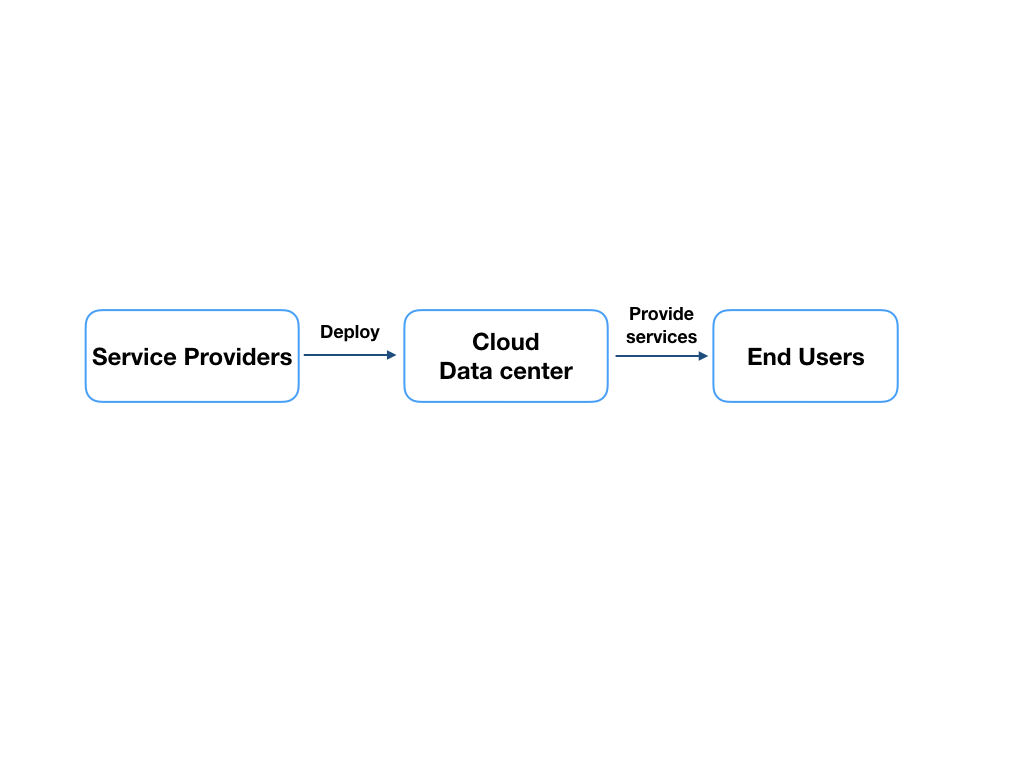
\includegraphics[width=0.6\textwidth]{pics/stakeholders.png}
	\caption{Stakeholders of Cloud computing \cite{Jennings:2015ht}}
	\label{fig:stakeholders}
\end{figure}

\bx{To give an example of how Cloud computing works (see Figure \ref{fig:stakeholders}), consider the case:} a \emph{Cloud provider} builds a data center containing thousands of servers. These servers connect with a network. 
To use these remote servers, \emph{Cloud user} (e.g an application provider), can deploy and access their applications (e.g Endnote, Google Drive and etc.) in these servers from anywhere in the world. Once the applications start serving, \emph{End users} can use them without installing on their local computers. Cloud providers charge fees from Cloud users for infrastructure. Cloud users charge fees from End users for using applications. \tran{Therefore, from cloud providers' perspective, both accommodating more applications and reducing energy consumption lead to the increase of profit.}

\bx{The major expense of a cloud provider is energy consumption \cite{Kaplan:up01fR-k} and physical machines (PMs) (e.g servers) contribute to a majority of the energy.} As shown in Figure \ref{fig:consumption}, both the cooling system and physical machines (PMs) account for 40\% of energy. However, PMs' energy efficiency are low on average  \cite{Hameed:2016cmb}.
The reason for low energy efficiency is the disproportion between the utilization of PMs and the energy consumption of PMs. \howto{For example, when CPU utilization of a PM is 15\%, the energy consumption of the PM is 70\% of its peak time.} Therefore, 
cloud providers can reduce the energy consumption by improving the utilization of PMs.


\tran{In order to solve the low energy efficiency caused by low utilization of PMs, cloud providers use a resource management system to manage the applications.}

\begin{figure}
	\centering
		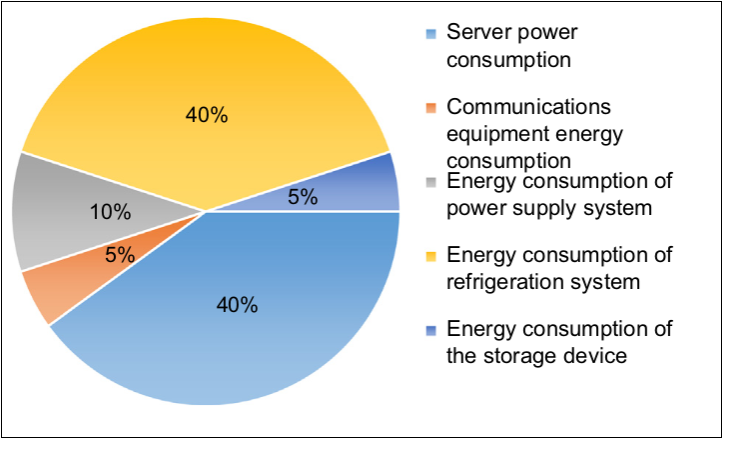
\includegraphics[width=0.35\textwidth]{pics/energyConsumption.png}
		\caption{Energy consumption distribution of data centers \cite{Rong:2016js}}
		\label{fig:consumption}

\end{figure} 

\section{Cloud Resource Management}
\label{sec:resource_management}
\bx{Cloud resource management is a process of allocating computation resources (e.g CPU and memory) to Cloud users to run their applications. Meanwhile, resource management aims to achieve low energy consumption in cloud} \cite{Jennings:2015ht}.

Resource management applies two types of virtualization: virtual machine (VM) and container on four management steps (see Section \ref{sec:statement}): collecting PMs' utilization data, analyzing available PMs, deciding the placement of applications, and executing the placement. Furthermore, in the third step of placement decision, resource management has three common scenarios: initial placement, periodic placement, and dynamic placement. Resource management uses distinct server consolidation strategies on these placement scenarios based on different virtualiazation technologies to achieve energy efficiency. 

This section will first introduce and compare two types of virtualization: VM-based and container-based and then illustrate 
three placement decision scenarios. 

\subsection{Virtualization Technologies}
\label{sec:virtualization}

\bx{Resource management uses virtualization technologies \cite{Uhlig:2005do} to achieve a finer granularity management than the traditional way.} In comparison with traditional management -- allocating an application to a PM -- virtualized management partitions PM's resources (e.g. CPU, memory and disk) into several independent units and allocates applications into these units. 
The most common units are virtual machines (VMs) and containers.

Virtualization technology rooted back in the 1960s' was originally invented to enable isolated software testing. Because VMs can provide good isolation for applications running without interfering with each other \cite{Somani:2009ho}. Soon, people realized that virtualization can improve the utilization of hardware resources: with each application deployed in a VM, a PM can run multiple applications. 

The next two sections illustrate two classes of virtualization (see Figure \ref{fig:comparison}): VM-based and container-based virtualization and then compares the two virtualizations.

\begin{figure}
	\centering
	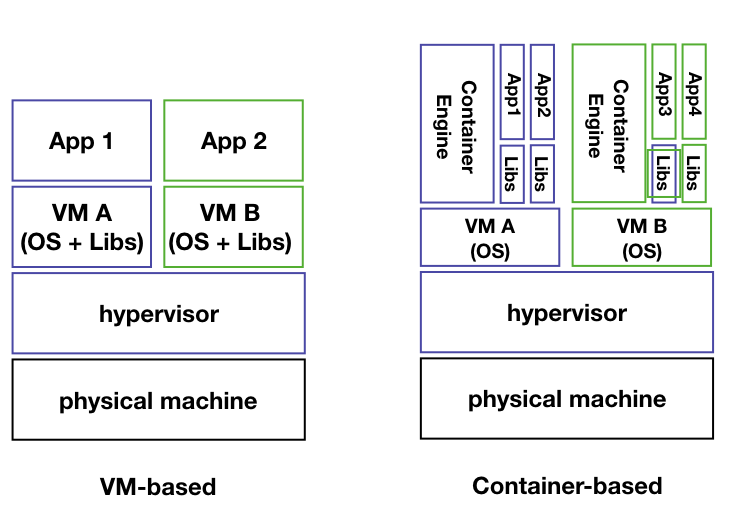
\includegraphics[width=0.7\textwidth]{pics/comparison.png}
	\caption{A comparison between VM-based and Container-based virtualization \cite{Piraghaj:2016bw}}
	\label{fig:comparison}
\end{figure}

\subsubsection{VM-based Virtualization} 

\bx{A VM-based virtualization has three-layers of structure: PM-Hypervisor-VM (see Figure \ref{fig:comparison} left-hand side).} 
The hypervisor or the virtual machine monitor (VMM) is a software layer on top of PM. A hypervisor arbitrates accesses to the PM's resources so that VMs can share resources on the PM. Some implementations of VM-based hypervisors such as Xen \cite{Barham:2003cj}, KVM \cite{Kivity:2007wu}, and VMware ESX \cite{Waldspurger:2002db} dominate this field in recent years. On of top of hypervisor, \textbf{VMs} are the fundamental resource management units. A VM allows independent Operating System (OS) to run on it.  

In addition, hypervisors support dynamic migration techniques (e.g pre-copy \cite{Clark:2005ud} and post-copy \cite{Hines:2009fv}) that can move VMs from one PM to another. Therefore, resource management can improve the utilization of a PM by migrating VMs to that PM.


\subsubsection{Container-based Virtualization} 

\begin{figure}
	\centering
	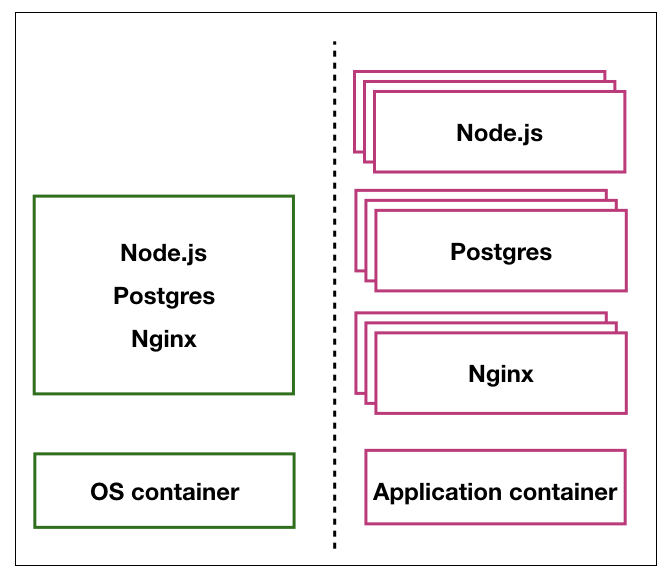
\includegraphics[width=0.4\textwidth]{pics/container_OS_APP.png}
	\caption{A comparison between OS container and Application container \cite{Piraghaj:gb}}
	\label{fig:comparison_container}
\end{figure}

\bx{A Container-based virtualization has four-layers of structure: PM-Hypervisor-VM-Container (see Figure \ref{fig:comparison} right-hand side).} Container-based virtualization is also addressed as operating-system-level virtualization because containers run on top of VMs. Specifically, container-based virtuliazation includes two classes: OS container and application container \cite{Piraghaj:gb}. 

\bx{OS containers (Figure \ref{fig:comparison_container} left-hand side) have a one-on-one relationship with VM.}
Multiple applications run inside an OS container. Three implementations of OS-level of containers: OpenVZ, Google's control groups, and namespace \cite{Rosen:2013wt} are widely used in Google and Facebook.

\bx{Application containers (Figure \ref{fig:comparison_container} right-hand side) have a many-to-one relationship with VM.} A single application runs on an application container. Major implementations such as Docker, Rocket and Kubernetes \cite{Bernstein:2014ur} are very popular in the software industry. 

\bx{In comparison with OS container, an application container is much more flexible because each container has its separated environment (e.g. libraries) for applications.} Furthermore, application containers provide a finer granularity of resource management by enabling an application level of operations including deployment, scaling, and migration.  

Notice that, in the following content, we use ``container'' to represent ``application container''. 
We do not discuss Os container because it is very similar to a VM.


\subsubsection{Comparison between Container-based and VM-based Virtualization} 
\label{sec:comparison_container_vm}
\bx{This section summarizes three disadvantages of VM-based virtualization in terms of energy efficiency and shows how container-based can overcome these disadvantages based on several research~\cite{Felter:2015ki, Xavier:2013fy, Dua:2014bw}.}  


Some main disadvantages in VM-based virtualization are listed as follows:
\begin{itemize}
	\item Resource over-provisioning \\
	\bx{Cloud users tend to reserve more resources for ensuring the Quality of Service at peak hours \cite{Chaisiri:2012cva}} The over reserved resources lead to low resource utilization. Cloud users do not completely rely on auto-scaling because auto-scaling is more expensive than reservation. However, the peak hours only account for a short period, therefore, for most of the time, resources are wasted.

	\item Unbalanced usage of resources \\
	\bx{Specific applications consume unbalanced resources.} The unbalanced resources lead to a vast amount of resource wastage \cite{Tomas:2013iv}. For example, computation intensive tasks consume much more CPU than RAM; a fixed type of VM provides much more RAM than it needs. Because the tasks use too much CPU, they prevent other tasks from co-allocating. This also causes wastage.

	\item Heavy overhead of VM hypervisors and redundant operating systems (OSs) \\
	\bx{Heavy overhead of  hypervisors and redundant OSs running in the PM also causes huge resource wastage.} Traditional VMs provide a complete independent environment that includes its own OS and libraries for deploying software. However, as most applications only require a general OS such as Windows or Linux, multiple duplicate OSs running in the system is a waste of resource.
\end{itemize}


Some key characteristics of containers can help overcome the above disadvantages of VMs.

The following two characteristics can overcome the heavy overhead of VM hypervisors and reduce the redundant OSs.
\begin{itemize}
	\item Container-based virtualization has lightweight management that generates much less overhead than a VM hypervisor. 
	\item Container-based virtualization shares OSs. Therefore, fewer VMs reduce overheads of multiple OSs.

	\item Container-based virtualization naturally supports vertical scaling while VM-based virtualization does not. Vertical scaling means a container can dynamically adjust its resources under the host's resource constraint. This feature offers a fine granularity management of resources. 

\end{itemize}

	Vertical scaling can overcome the resource over-provisioning by dynamically adjusting the size of containers. Furthermore, the size of container reflects the requirement of the application. We can achieve a balanced usage of resources by using appropriate placement algorithm.


\bx{In summary, container-based virtualization has the potential to further improve the energy efficiency than VM-based virtualization.} No matter which virtualization technology is used, the cloud often deals with three placement decision scenarios. 




\subsection{Placement Decision Scenarios}
\label{sec:scenarios}

\bx{Three placement decision scenarios \cite{Svard:2015ic, Mishra:2012kx}: initial placement of applications, periodic placement of applications, and dynamic placement of applications (see Figure \ref{fig:management}).}

\begin{figure}
	\centering
	\begin{subfigure}[b]{0.9\textwidth}
		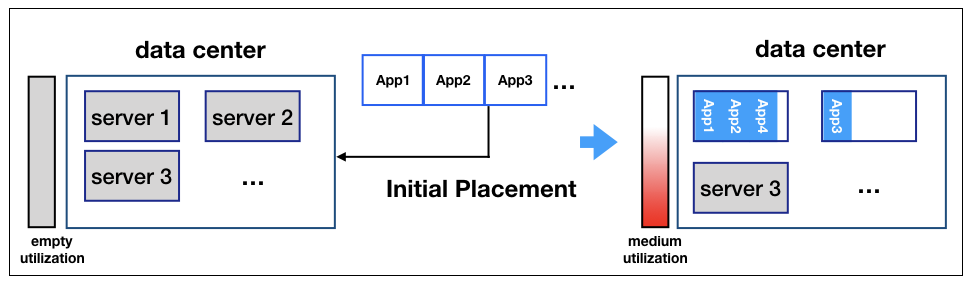
\includegraphics[width=\textwidth]{pics/initial_placement.png}
		\caption{Initial placement of applications}
	\end{subfigure}
	\begin{subfigure}[b]{0.9\textwidth}
		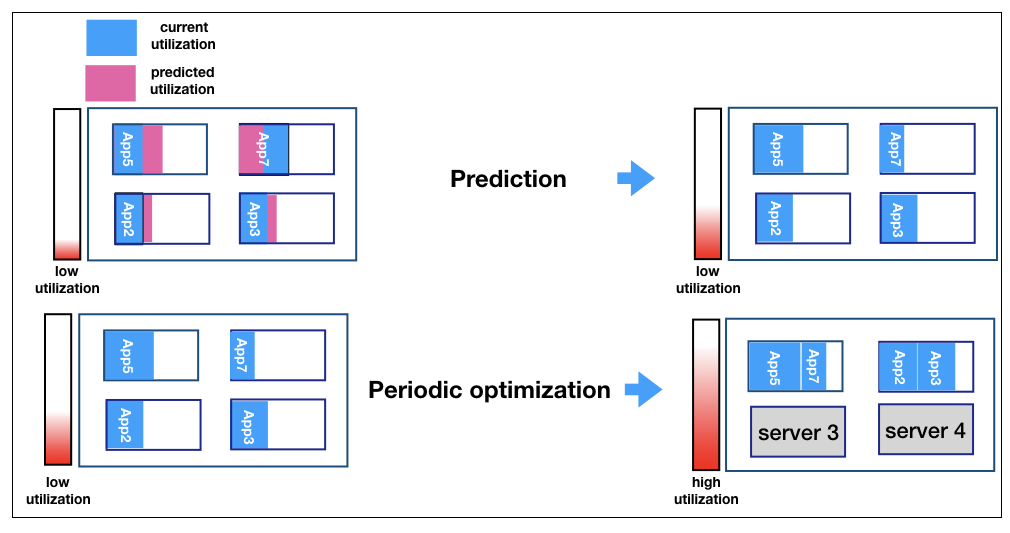
\includegraphics[width=\textwidth]{pics/periodic_optimization.png}
	\caption{Periodic placement of applications}
	\end{subfigure}
	\begin{subfigure}[b]{0.9\textwidth}
		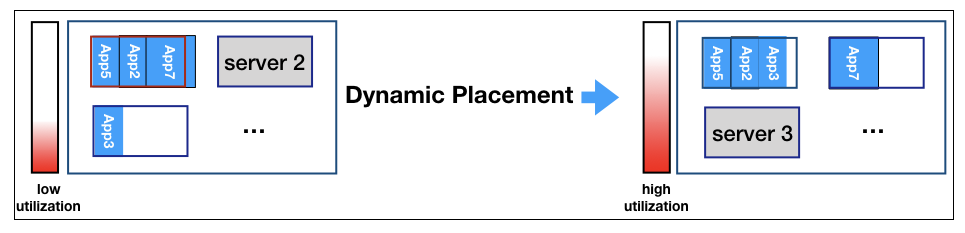
\includegraphics[width=\textwidth]{pics/dynamic_placement.png}
	\caption{Dynamic placement of applications}
	\end{subfigure}
	\caption{Three scenarios of placement decision}
	\label{fig:management}
\end{figure}

\paragraph{Initial Placement of Applications} is applied when new applications arrived. The task is to place applications into a set of PMs \cite{Mishra:2012kx} so that PMs satisfy all applications' resource demands and minimize the energy consumption.



\paragraph{Periodic Placement of Applications} is applied periodically to adjust the current placement of applications. The task is to re-place the current applications so that resource management minimizes the energy consumption and minimizes the cost of migration.

\paragraph{Dynamic Placement of Applications} is applied in two scenarios \cite{Mishra:2012kx}: Overloading and underloading. Overloading is a scenario where the total demands of applications in a PM are higher than the PM's resources. Therefore, the PM causes a degradation in one or more applications' performance. Underloading is a scenario where the PM is running in low utilization. In both scenarios, resource management moves the applications from one PM to another PMs in an on-line fashion~\cite{Borodin:2cY4439E}.

Next section will discuss general server consolidation strategies.

\subsection{Server Consolidation Strategy}
\label{consolidation}

\begin{figure}
	\centering
	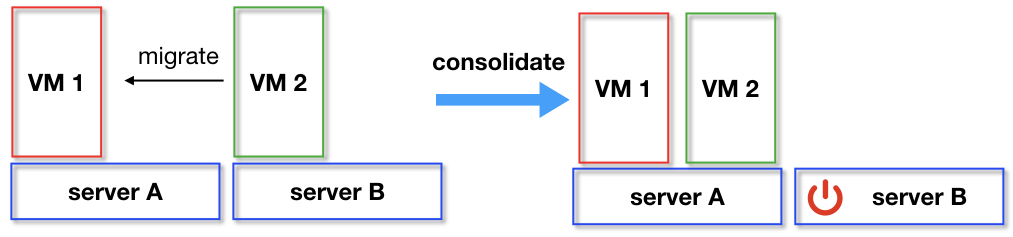
\includegraphics[width=0.7\textwidth]{pics/consolidate.png}
	\caption{A Server Consolidation example: Initially, each PM runs an application wrapped with a VM in a low resource utilization state. After the consolidation, both VMs are running on PM A, so that PM B is turned off to save energy \cite{Barroso:2007jt}.}
	\label{fig:consolidation}
\end{figure}


\bx{Server consolidation is a resource management strategy that aims to improve the utilization of PMs and reduce the energy consumption.} We use VM-based virtualization as an example: a general step of server consolidation is shown in Figure \ref{fig:consolidation}, a number of VMs is migrated to fewer number of PMs. Resource management applies Server consolidation to solve 
the low utilization of PMs called PM sprawl~\cite{Khanna:2006vq}.

% \subsubsubsection{Model}
\begin{figure}
	\centering
	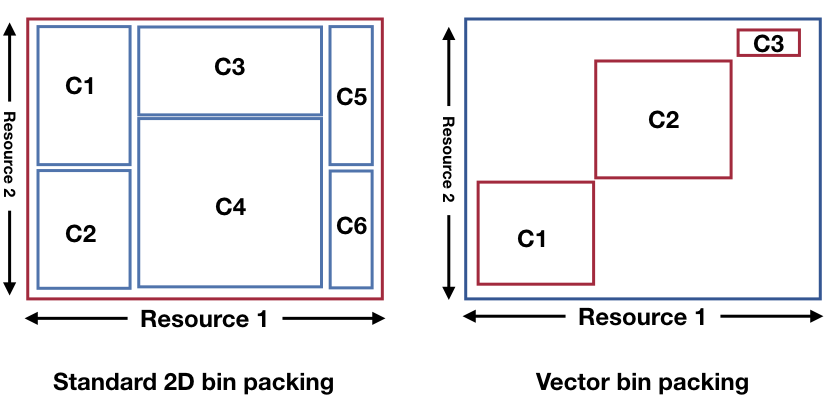
\includegraphics[width=0.6\textwidth]{pics/bin_packing_problem.png}
	\caption{A comparison between standard bin packing and vector bin packing}
	\label{fig:bin_packing_problem}
\end{figure}

\subsubsection{Types of Server Consolidation}

% Three major benefits of virtualization make it be the first choice for web-based application consolidation: No reliance on hardware, easy to provision and live migration.

\bx{Server consolidation can be done in two ways: Static and dynamic \cite{Xiao:2015ik, Verma:2009wi} based on different scenarios.} Initial placement and periodic placement involve large number of variables, therefore, they are very time-consuming job and often conducted in an off-line fashion. Dynamic placement requires a fast decision-making to place one application to PMs. Thus, resource management uses a dynamic server consolidation strategy to handle the scenario. 



\section{Evolutionary Computation}
\bx{Evolutionary Computation (EC) algorithms are artificial intelligent algorithms that are inspired by biological mechanisms of evolution, social interactions and swarm intelligence.} They are famous for strong search ability because they have several distinguished characteristics such as the use of a population-based search and the ability of avoiding local optima. EC algorithms have been applied successfully to solve a variety of real-world problems \cite{Engelbrecht:dm}, especially, combinatorial optimization problems.

% A common process of EC algorithms is as follows. Initially, the population are randomly generated in the search space. During the evolution process, the population
% explores according to the evaluation of a or multiple predefined fitness functions. At the end of the evolution, the individual with the best fitness value is selected as the output.

\bx{Researchers have proposed a variety of EC algorithms \cite{Yao2006} to solve optimization problems.} The majority of current EC algorithms descends from three major approaches: \emph{genetic algorithms (GAs)}, \emph{particle swarm optimization (PSO)} and \emph{genetic programming (GP)}. 


This section will first introduces these three important EC algorithms that we would like to use in our future work. Then, we will review a number of EC algorithms that are used in combinatorial optimization problems. From these problems, we will conclude some of the advantages of using EC algorithms in solving resource allocation problem in clouds.

\subsection{Genetic Algorithms (GAs)}
% GA \cite{Holland:1962fy} was introduced by Holland. Since then, a large number of applications \cite{DeJong:1992vk, DeJong:1992ws} have applied GA  as their search mechanism. 
\bx{GA is a population-based search algorithm \cite{Vose:1993iu}.} In GA, the solution of a problem is coded as a vector of numbers called chromosome or individual. A GA searches for the best solution by iteratively changing the values in the chromosome. 

\bx{We describe a general GA procedure as follows.} In the beginning, a population of chromosomes which represents the solutions of the problem are often represented as a fixed length string. Each entry or bit can be continuous, discrete or even alphabets depending on the problem.  The evolution often starts from randomly generated population followed by an iterative process called generation.  In each generation, the fitness value of chromosomes is evaluated according to a defined fitness function.  Then, genetic operators such as mutation and crossover are applied on the solutions so that they are modified. As a search mechanism, these operators move solutions to explore the search space. New generations of solutions are then evaluated by the fitness function.  This evolutionary procedure ends when a predefined generation number or a satisfactory level of fitness has been reached.

\begin{figure}
	\centering
	\begin{subfigure}[b]{0.44\textwidth}
		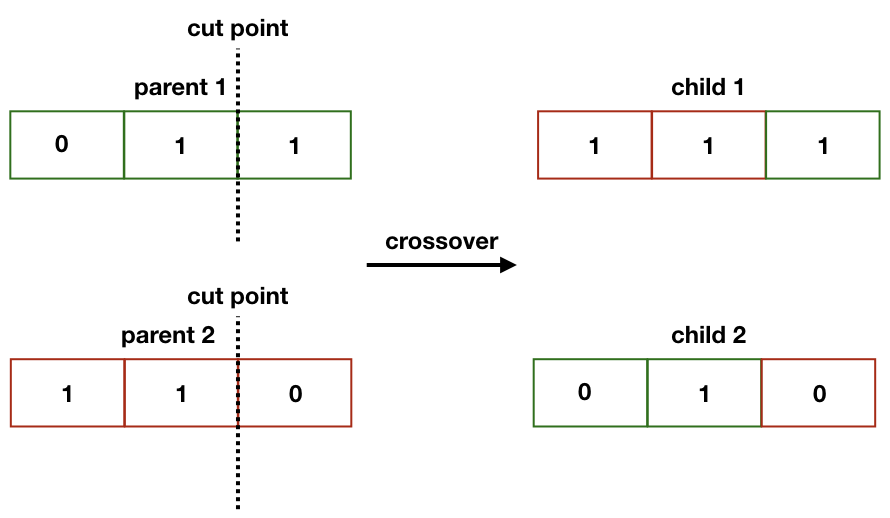
\includegraphics[width=\textwidth]{pics/crossover.png}
	\caption{Crossover}
	\end{subfigure}
	\begin{subfigure}[b]{0.44\textwidth}
		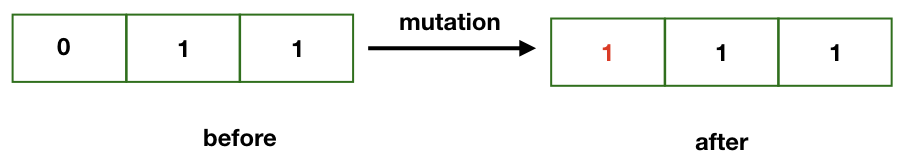
\includegraphics[width=\textwidth]{pics/mutation.png}
	\caption{Mutation}
	\end{subfigure}
	\label{fig:operators}
\end{figure}

\bx{GA-based algorithms are suitable for off-line combinatorial optimization problems.} Different from traditional algorithm such as Integer linear programming (ILP) technique, a GA-based algorithm bypasses the complicated procedure of tunning parameters by searching through the solution space of a problem. Although a GA-based algorithm does not guarantee a global optima solution, a GA-based algorithm normally can provide a near-optima solution within feasible amount of time. Although a GA-based algorithm spends less time than an ILP, it still takes too long time than an on-line problem requires. Therefore, we will consider use a GA-based algorithm in the first and second objectives: initial placement of applications and periodic placement of applications. 

GA-based algorithms have been applied to a variety of combinatorial optimization problems such as the assembly line balancing problem \cite{Anderson:1994io}, scheduling in Grid computing \cite{Zomaya:2005bb} and resource allocation problem in clouds \cite{Wilcox:2011ea}. Specifically, we will discuss the literature that applied GA-based algorithms in the server consolidation strategies in Section \ref{sec:related_work}. 

Next section will introduce another popular algorithm: particle swarm optimization (PSO). 


% Evolutionary programming, introduced by Fogel \cite{Fogel:1962wv}, was originally designed to generate artificial intelligence. 
% Evolutionary strategies as developed by Rechenberg \cite{Rechenberg:a_aZDNtZ} and Schwefel \cite{Schwefel:Nd2pzTwG}, were initially designed with the goal of solving difficult discrete
% and continuous, mainly experimental, parameter optimization problems \cite{Klockgether:1970tw}. 

\subsection{Particle Swarm Optimization (PSO)}
\bx{PSO is a meta-heuristic algorithm inspired by the social behavior of birds \cite{Eberhart:1995tj}.} In PSO, each individual -- a particle -- searches the solution space. The underlying phenomenon of PSO is to use the collective knowledge to find the optimal solution.

\bx{We describe the procedure of PSO as follows.} At the initial state, each particle has a random initial position in the search space that is represented by a vector $\vec{x}_i = (x_{i1}, x_{i2}, \dots, x_{iD})$, where \emph{D} is the dimension of the search space. A particle has a velocity as $\vec{v}_i = (v_{i1}, v_{i2}, \dots, v_{iD})$. The velocity is limited by a threshold $v_{\max}$ so that for any $i$ and $d$, $v_{id} \in [-v_{\max}, v_{\max}]$. During the search process, each particle maintains a record of its best position so far, called the \emph{personal best} ($pbest$). The best position among all the personal best positions of its neighbors is the \emph{global best} ($gbest$). The position and velocity of each particle are updated according to the following equations:
\begin{equation}
\label{eq:updatePosition}
x^{t+1}_{id} = x^{t}_{id} + v^{t+1}_{id},
\end{equation}

\begin{equation}
\label{eq:updateVelocity}
v^{t+1}_{id} = w \cdot v^{t}_{id} + c_1 \cdot r_{1i} \cdot (p_{id} - x^t_{id}) + c_2 \cdot r_{2i} \cdot (p_{pg} - x^i_{id}).
\end{equation}

Here, $t$ is the index of iteration. $d$ is the index of dimension. The inertia weight $w$ is used to balance the local search and global search abilities. The parameters $c_1$ and $c_2$ are the acceleration constants. $r_{1i}$ and $r_{2i}$ are random constants following the uniform distribution in the interval $[0, 1]$. $p_{id}$ and $p_{gd}$ denote the values of $pbest$ and $gbest$ in the $d^{th}$ dimension of the $i^{th}$ particle.

\bx{PSO-based algorithms are also suitable for combinatorial optimization problems.} Although PSO was originally developed for optimizing problems with continuous representations (e.g. real-value), the recent development of PSO support the discrete problem as well. Specifically, the binary PSO \cite{Kennedy:1997hd} is designed for binary problems; the discrete PSO \cite{Liao:2007dl} is designed for scheduling problems; and a Combinatorial PSO \cite{Jarboui:2007in} is developed for problems with integer representation. In the literature, PSO-based algorithms have also been applied for resource allocation problem \cite{Xiong:2014jq}. We will discuss these approaches in Section \ref{sec:related_work}.


\bx{Compared with GA-based algorithms, PSO-based algorithms have a faster convergence speed.} However, PSO-based algorithms are more easier to be stuck at local optima for large dimensional problems than GA-based algorithms. Therefore, sometimes PSO-based algorithms can be used in dynamic problems if the number of variables is small. More often, PSO-based algorithms are applied in off-line problems like GA. Therefore, we will also consider using PSO in the first and second objectives.

Next section will introduce the genetic programming-based hyper-heuristic (GP-HH), which is suitable for dynamic problems.

\subsection{Genetic Programming-based Hyper-heuristic (GP-HH)}

Genetic programming \cite{1992gppc.book.....K} is an evolutionary computation technique, inspired by biological evolution, to automatically find 
computer programs for solving a specific task. In a GP population, each individual represents a computer program. In each generation, these programs are evaluated by a predefined fitness function, which accesses the performance of each program. Then, individuals will go through several genetic operators such as selection, crossover, and mutation. A number of top individuals will survive to the next generation while others will be discarded. The major difference between GA and GP is that each GP individual is represented as a tree with variant depth instead of a string. This representation is particular suitable for a program. For example,  a GP individual is shown in Figure \ref{fig:gp_program} which is a program x + max(y $\times$ 2, -2). The variables \{x, y\} and constraint \{-2, 2\} are called terminal of the program. The arithmetic operations \{+, $\times$, max \} are called functions in GP. A GP individual is a specific combination of elements in a terminal set and a functional set. In order to observe the relationship between a function and its subtrees, the GP programs are usually presented to human users by using the $prefix$ notation similar to a Lisp expression, for example, x + max(y $\times$ 2, -2) can be expressed as (+ (x (min ($\times$ y 2) -2 ))).

\begin{figure}
	\centering
	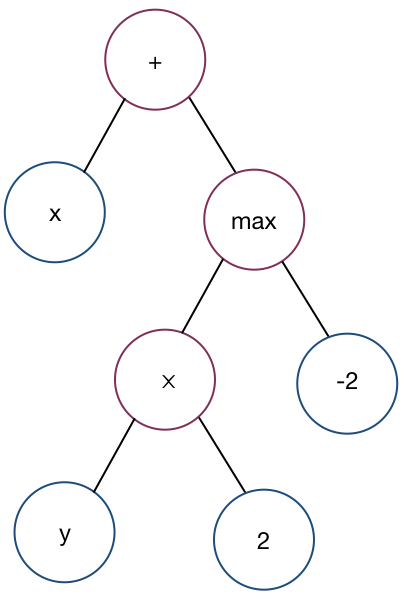
\includegraphics[width=0.3\textwidth]{pics/gp-tree.png}
	\caption{GP program that represents x + max(y $\times$ 2, -2)}
	\label{fig:gp_program}
\end{figure}


GP-based hyper-heuristics (GP-HH)  has been applied in many applications such as Job shop scheduling to evolve dispatching rules \cite{Nguyen:2014eu}. The term hyper-heuristics \cite{Cowling:2000ek} means ``heuristics to choose heuristics''.
\emph{Dispatching rule} is essentially a heuristics \cite{Panwalkar:1977fw} used in a scheduling context. 
Resource allocation problems are also in the scheduling category and they are often modeled as bin packing problems. 
GP-HH has been applied in generating heuristics for bin-packing problems \cite{Poli:2007kt,Sim:2013fe,Burke:2012gs}. These research studies have shown that GP-HH can generate excellent heuristics which have equal or better performance than human designed heuristics.

In the Cloud computing context,  Cloud resource allocation usually has extra constraints such as multi-dimensional resources, migration costs, heterogeneous PMs, etc. These constraints make the Cloud resource allocation problem much harder than original bin packing \cite{Mann:2015ua}. Therefore, traditional bin packing approaches such as First Fit Decreasing, Best Fit, etc, cannot perform well in this context.  GP-HH, therefore, is a promising technique that can be used to automatically generate heuristics under multiple constraints.

\subsection{EC Algorithms in Combinatorial Optimization}
This section will review a number of EC algorithms in two typical combinatorial optimization fields: cloud computing resource allocation and job shop scheduling. 

\paragraph{Cloud Computing Resource Allocation}
Traditional cloud computing resource allocation includes six categories \cite{Guzek:2015ds}: cloud brokering, VM placement, service placement and workflow scheduling are typically static problems; server load balancing and cloud capacity planning are dynamic problems. EC algorithms have been applied in problems in each of these categories. This section will briefly review approaches used in these problems except VM placement. We will explicitly discuss VM placement in Section \ref{sec:related_work}.

\vspace{5mm}

In cloud brokering problem, a cloud broker is an intermediary between cloud users and cloud providers. Cloud brokers estimate the resource requirements and choose resources for cloud users. The objective of cloud brokering is to minimize the cost for cloud users as well as guarantee the quality of service (QoS) of cloud users' applications.

Frey et al \cite{Frey:2013gp} propose a GA approach (CDOXploer) for finding near-optimal cloud deployment architectures and runtime reconfiguration rules for softwares. Their approach takes into account VM types, the number of VMs, and the scaling policies of VMs. CDOXplorer minimizes response times, costs, and SLA violations in order to satisfy the requirement of cloud users.  In comparison with Frey's centralized approach, Iturriaga et al \cite{6681297} propose an Evolutionary Algorithm (EA) with distributed sub-populations. In each sub-population, they applied a Simulated Annealing (SA) method to find the local optimal solution. The proposed algorithm is shown outperform than the reference list scheduling algorithm in both computation time and performance (maximizing the profit of a broker).

\vspace{5mm}

In service placement problem, cloud users would like to optimize the costs and performance (e.g QoS) of their services. Compared with cloud brokering problem, service placement less focuses on resource allocation but more focuses on the latencies between locations. Cloud users need to decide the locations of services and the number of services \cite{Guzek:2015ds}. 

Tan et al \cite{Tan2017} propose an aggregation approach with binary PSO to solve the service placement problem with two objectives: minimizing cost and minimizing the response time. They find that the single-objective algorithm can only provide one solution for each run, hence, single-objective algorithm cannot provide alternatives when cloud users do not have preferences. Therefore, they develop an NSGA-II based approach \cite{Tan2016} that uses Pareto front approach to find a set of non-dominated solutions. They conclude that multi-objective evolutionary algorithms are suitable for the service placement problem.

\vspace{5mm}

The workflow scheduling problem allocates a set of dependent services, organized as a directed acyclic graph (DAG). The objectives of workflow scheduling are minimizing makespan and cost. The major difference between workflow scheduling and service placement is the extra constraint on the order of services. Another difference is that workflow scheduling rarely considers the latency issue. Compared with cloud brokering problem, workflow scheduling problems have additional dependencies between applications.

 Tsai et al \cite{Tsai:2013fn} develop an Improved Differential EA (IDEA) to solve the multi-objective scheduling problem. They represent the solution as a permutation of subtasks. They also design a crossover operator that only changes the resource allocation of subtasks and a mutation operator that changes the task order. They compare IDEA with NSGA-II, SPEA2, and DEA in two test scenarios. The results show their approach outperforms than other EC algorithms. 

\vspace{5mm}

Capacity planning problems estimate the future load of VMs and PMs before allocating resources.
The major objectives is to optimize the QoS while minimizing the cost of users. Different from above problems, the capacity planning problem is often treated as a dynamic problem. 

Kousiouris et al \cite{Kousiouris:2013vg} propose an artificial neural (ANN) network-based framework to predict the load of a GNU Octave system. They use a GA to create the structure of ANN and the ANN is encoded using a bit-string representation. The algorithm can be trained off-line and test on-lien. Therefore, it is well-suit for a dynamic problem.

\vspace{5mm}

Similar as the capacity planning problem, server Farm Load Balancing problem is also a dynamic problem. The task is to dispatch incoming requests to a set of machines. The major objective is to satisfy the QoS (e.g. makespan) of cloud users.

Laredo et al \cite{Laredo:2014db} propose an on-line and decentralized scheduler for distributing Bag-of-task kind of workloads to heterogeneous infrastructures. Their approach mimics the behavior of sandpile. They manage cloud resources (PMs) by segmenting resources and assign each segmentation with a monitor called agent. These agents interact with their neighbors (predefined) and share their information about resources. Tasks arrive to PMs and accumulate as grains of sand. When an agent detects an unbalance between a segment of resources and its neighbors, it triggers an avalanche. They test the system with very large scale problems: 2048 PMs and 2048 tasks and achieve at least five times better in terms of makespan and throughput than a round robin algorithm.

Server Farm load balancing is very similar to another classic problem: job shop scheduling (JSS). They both dispatch a set of jobs to a set of machines except load balancing problem focus more on computing resources such as CPUs and memories. In the next section, we will introduce JSS and the EC methods applying on JSS.
\paragraph{Job Shop Scheduling}
Job shop scheduling (JSS) problems \cite{Potts:2009eb} dispatch a set of jobs to machines. A job goes through a predetermined sequence of operations in order to finish its tasks. Each machine can only process a specific operation. Therefore, we need to make intelligent decisions to schedule these jobs in order to finish processing jobs before their due dates.

JSS problems can be divided into two categories: static and dynamic. In static JSS problems, all properties of jobs and machines are known in advance. In dynamic JSS problems, properties of jobs are unknown.  

The state-of-the-art approaches for static JSS problems use meta-heuristics. Examples of meta-heuristics approaches to JSS include Tabu search \cite{AmaralArmentano:2000dk}, GA \cite{Zhou:2009dq} and etc. These meta-heuristics can handle large JSS problem instances effectively. 

Dynamic JSS problems often apply small heuristics such as dispatching rules \cite{Branke:2016wy} because dispatching rules have short reaction times and can quickly deal with unforeseen changes in an on-line event. For example, a SPT (shortest processing time) selects the job with the shortest processing time waiting at the available machine. Apart from simple dispatching rules, composite dispatching rules (CDRs) \cite{Jayamohan:2004kq} combine several simple dispatching rules to achieve higher performance. 

However, it is difficult to design dispatching rules for dynamic JSS problems. This is because, first, no single dispatching rule is more effective than others for all JSS problems. Second, a real-world dynamic JSS problem is changing over time, e.g. machines are added and removed. Therefore, designing dispatching rules often requires domain knowledge. 

To design dispatching rules more effectively, researchers use a hyper-heuristic technique to automatically generate dispatching rules. Specifically, a great number of hyper-heuristic approaches to JSS problem uses Genetic Programming (GP) technique called GP hyper-heuristic (GP-HH). GP-HH represents dispatching rules with a tree-based representation and these dispatching rules can be interpreted as priority-based dispatching rules. GP-HH approaches generally outperform manually designed dispatching rules for both static and dynamic JSS problems \cite{Branke:2016wy}. 

In comparison between the dynamic JSS problem and the dynamic placement of applications, they share many similarities. First of all, they are both on-line problems that require a fast reaction. Second, they both dispatch jobs to machines. The differences are the dynamic JSS problem normally does not care the amount of resources that a job consumes. The dynamic placement not only considers the resource requirement of jobs but also the remaining of resources in Physical machines (PMs). Another difference is that the jobs in dynamic JSS go through a route of machines while the jobs in dynamic placement stay at one machine.

The similarities inspire us to apply GP-HH approach on the dynamic placement of applications problem.

\vspace{5mm}


In conclusion, EC-based algorithms have been widely used in resource allocation problems in cloud for both static problems and dynamic problems. Specifically, meta-heuristics such as GA and PSO are more suitable for static problems and hyper-heuristics such as GP are suitable for dynamic problems. 
We conclude several advantages of EC approaches. First, EC-based algorithms rely on searching in the solution space, which bypass the complexity of finding the exact mathematical approach. Second, EC-based algorithms are population-based algorithms, which can find near-optimal solutions within a feasible amount of time.
Next section will provide the literature of traditional approaches and EC-based approaches on server consolidation strategies in terms of two virtualization: container and VM. 


\section{Related Work}
\label{sec:related_work}
Related work discusses the server consolidation strategy and the studies of consolidation strategies on three placement decision scenarios: initial placement, periodic placement, and dynamic placement. 


\subsection{Initial Placement of Applications}
\label{sec:initial}

This section first discusses server consolidation strategies on container-based virtualization and VM-based virtualization.

\subsubsection{Container-based Initial Placement of Applications}
\label{container-based-placement}
This section will discuss existing approaches for container-based initial placement. Then, we will describe a potentially way of modeling energy consumption in container-based virtualization: a bilevel model. Last, we will illustrate a number of algorithms to solve bilevel optimization problems. 


\paragraph{Existing Approaches}

\bx{We discuss two research works on container-based virtualization: Piraghaj et al \cite{Piraghaj:2016bw} and Mann \cite{Mann:2016hx} on their similarities and differences.} Two papers both consider two resources: CPU and memory. The constraints on these resources are the containers cannot exceed the resources in their located VMs. Both research do not include the balance of CPUs and memories. In contrast, in most VM-based approaches (discussed in next section) consider the balance.

\bx{The first difference between two papers is that Mann considers the overheads of VM.} Mann models the overhead as a constant value of CPU utilization but he mentioned more sophisticated models can be more realistic. On the other hand, Piraghaj et al \cite{Piraghaj:2016bw} adopt a widely used VM-based linear energy model~\cite{Xavier:2017jl} and does not consider the overheads of VM. 

The second difference is their resource management architectures. The architecture in Piraghaj's research allows adjusting 
the size of VMs when allocating new applications, while in Mann's work, containers runs on top of a traditional IaaS where containers must choose to allocate to a type of VM. 

The third difference is their distinct ways to achieve initial placement based on their different architectures of resource management. Piraghaj considers the initial placement a two-steps procedure: containers to VMs and VMs to PM. Because their resource management allows cloud providers to customize the size of VMs, in the first step, they must first determine the size of VM. Piraghaj performs clustering technique on historical workload data from Google Cluster Data. In this way, Piraghaj suggests that the applications with similar workload pattern can be categorized into the same group. In the placement step, Piraghaj designs a simple heuristic: in both VM and PM levels, they apply First Fit algorithm. Then, the containers are allocated to certain size of VMs. Piraghaj claims that their main contribution is not the placement strategy but an architecture for container-based resource management. On the other hand, Mann realizes this two-levels of placement are interact with each other, therefore, container-VM and VM-PM must be considered collaboratively. Specifically, the initial placement of applications becomes three parts: 

\begin{itemize}
	\item VM size selection for containers
	\item Container placement
	\item VM placement
\end{itemize}

% However, another concern is ``why not placement as many containers as possible in a single VM which minimizes the overhead of hypervisor''. The paper gives an answer of ``Too big VMs limit the consolidation possibilities''. 
In order to prove interaction of two-levels of placement, Mann fixed a VM placement algorithm and tested a series of VM selection algorithms such as simple selection \cite{Ganesan:2012eb},  Multiple selection, Maxsize, Consolidation-friendly. Mann discovers that the final energy consumption varies with the selection algorithms. Mann claims that the performance is better when VM selection has more knowledge of the PMs' capacity. However, Mann's study only focuses on the partial placement with fixed VM placement algorithm. The answer of ``How these two-levels of placement interact ?'' is still undiscovered.


\bx{We have two reasons to propose a distinct approach from Piraghaj \cite{Piraghaj:2016bw} to solve the container-based placement problem.} First, Piraghaj's architecture can create arbitrary size of VM when requests arrive. In contrast, our assumption is that the container-based architecture is based on traditional IaaS, where fixed-size VMs provide the fundamental resources. Second, from the perspective of energy efficiency, the allocation of container and VM interact with each other. That is, the minimum number of VMs does not necessary lead to the minimum number of PMs, because the type of VMs also affect the results. Therefore, Piraghaj's approach cannot guarantee a near optimal energy consumption. This inspires us to simultaneously allocate containers and VMs. 

% In addition, both approaches do not consider the OS requirement of containers as a constraint. We argue that this is another critical reason for deploying containers into different VMs.

In order to solve the problem, we believe a promising way is to model the energy consumption in container-based virtualization as a bilevel optimization~\cite{Colson:2007bu} (described in the next section). Bilevel optimization represents the interaction so that a bilevel optimization algorithm can solve the energy consumption problem. Next section will introduce the basic structure of a bilevel model or a bilevel optimization.




\paragraph{Bilevel Optimization}
\label{bilevel}

A bilevel optimization \cite{Colson:2007bu} is a kind of optimization where one problem is embedded within another.
The general formulation of a bilevel optimization problem can be defined as: 

\begin{subequations}
\label{eq:bilevel}
	\begin{align}
	min_{x \in X, y} 	\quad F(x, y) \\
	s.t 			\quad G(x, y) \leq 0, \\
	min_y			\quad f(x, y) \\
	s.t 			\quad g(x, y)
	\end{align}
\end{subequations}

The lower-level problem is the function $f(x, y)$, where the decision variable is $y \in \mathbb{R}^{n_2}$. The upper-level problem is the function $F\{x, y\}$ where the decision variable is $x \in \mathbb{R}^{n_1}$.
The function $F : \mathbb{R}^{n_1} \times  \mathbb{R}^{n_2} \to \mathbb{R}$ and $f : \mathbb{R}^{n_1} \times  \mathbb{R}^{n_2} \to \mathbb{R}$ are the \emph{upper-level} and \emph{lower-level objective functions} respectively. The function $G : \mathbb{R}^{n_1} \times  \mathbb{R}^{n_2} \to \mathbb{R}^{m_1}$ and $g : \mathbb{R}^{n_1} \times  \mathbb{R}^{n_2} \to \mathbb{R}^{m_2}$ are called the \emph{upper-level} and \emph{lower-level constraints} respectively. 

Bilevel optimization problem has a hierarchical structure. This structure may introduce difficulties such as non-convexity and disconnectedness even for simple cases such as bilevel linear programming problems is strongly NP-hard \cite{Sinha:2013tn}. 

In practice, there are a number of problems that are bilevel in nature. For example, transportation related: work design, optimal pricing \cite{Brotcorne:2001je, Constantin:1995hu}, management: network facility location \cite{Sun:2008gq},  and engineering related: optimal design \cite{KirjnerNeto:1998ef}. 




\paragraph{Evolutionary Computation Approaches for Bilevel Optimization}

% A number of studies have been conducted on bilevel optimization \cite{Colson:2007bu,Dempe:2006jc}. 
Traditional approximation algorithms such as Karush-kuhn-Tucker approach \cite{Bianco:2009ej, Herskovits:2000be}, branch-and-bound \cite{Bard:1982gsa} are often applied to solve bilevel problems. Most of these approaches are not applicable when the problem size increases.
% Heuristics such as Evolutionary methods have been applied for solving bilevel optimization problem with higher level of complexity \cite{Yin:2000bt,Wang:2008kb}. 

Evolutionary methods have been applied to bilevel optimization problem since 90s. Mathieu et al \cite{Mathieu:2011dw} proposed an genetic algorithm (GA) based approach. It uses a nested strategy - the lower level is optimized with a linear programming method and the upper level apply a GA.

Oduguwa and Roy \cite{Oduguwa:2002kr} proposed a co-evolutionary approach for bilevel problems. Two population are co-operated to find the optimal solution, where each population handles a sub-problem. 

Wang et al \cite{Wang:2005fa} proposed an evolutionary algorithm based approach with a constraint handling technique.  Their approach is able to handle non-differentiability at the upper level objective function, but not in constraints and lower  level objective function. Later on, Wang proposed an improved version \cite{Wang:2011di} that shows better performance than the previous version.

Particle Swarm Optimization \cite{Li:2006br} was also used in solving bilevel problems.
A recent work is from Sinha et al \cite{Sinha:2013tn}, they propose a bilevel evolutionary algorithm (BLEAQ) works by approximating the optimal solution mapping between the lower level optimal solutions and the upper level variables.  BLEAQ was tested on two sets of test problems and the results were compared with WJL \cite{Wang:2005fa} and WLD \cite{Wang:2011di}. The results show BLEAQ is much faster than previous approaches.
One major drawback of evolutionary algorithms is its high computation cost which limits the problem size from growing bigger.

In conclusion, as the complexity of the problem, practical problems with bilevel nature are often simplified into a single-level optimization problem which can achieve a satisfactory level instead of optimal. Classic algorithms often fail because of the nature of bilevel problem such as non-linearity, discreteness, no-differentiability, non-convexity etc. EC algorithms have been successfully applied on bilevel problems.



\subsubsection{VM-based Initial Placement of Applications}
\label{initial_placement}
This section first describes a commonly used energy model for VM-based virtualization: Bin packing model. Then, we review a number of traditional approaches and EC-based approaches for VM-based initial placement . We mainly study the following five aspects: resources, power model, wastage model (balance between resources), objective, and algorithm.

\begin{table}[]
\centering
\caption{A Comparison of different models and approaches}
\label{vm-based-comparison}
\scalebox{0.7}{
\begin{tabular}{@{}lccccc@{}}
\toprule
\multicolumn{1}{c}{Research}                      & Resources        & Algorithm                     & \multicolumn{1}{l}{Power model} & Wastage model                             & \multicolumn{1}{l}{Objective} \\ \midrule
\multicolumn{1}{c}{Xu et al \cite{Xu:2010vh}}   & CPU and RAM      & GGA and Fuzzy multi-objective & Linear                          & balance  resources & three                         \\
\multicolumn{1}{c}{Gao et al \cite{Gao:2013gg}} & CPU and RAM      & Ant Colony Optimization       & Linear                          & balance  resources & Two                           \\
Ferdaus et al \cite{Ferdaus:2014ep}             & CPU, RAM, and IO & Ant Colony Optimization       & Linear                          & Sum of  resources          & Single                        \\
Wang and Xia \cite{Wang:2016eha}                & CPU and RAM      & MIP                           & Cubical                         & No                                        & Single                        \\
Wilcox et al \cite{Wilcox:2011ea}               & CPU and RAM      & GGA                           & Linear                          & Sum of resources          & Single    \\
Xiong and Xu \cite{Xiong:2014jq}               & CPU,RAM,Bandwidth,Disk      & PSO & Non-linear & Sum of resources          & Single \\ \bottomrule
\end{tabular}{}
}
\end{table}


\paragraph{Energy Model in VM-based Clouds: Vector Bin Packing Model}
\label{sec:vector_bin_packing}
\bx{Server consolidation is typically modeled as a Vector bin packing problem which is a variant of standard bin packing problem (see Figure \ref{fig:bin_packing_problem}).} Vector bin packing is also referred as multi-capacity \cite{Leinberger:1999fs} or multi-dimensional bin packing problem \cite{Xiong:2014jq}. Vector bin packing is particularly suitable for modeling resource allocation problems where there is a set of bins with known capacities and a set of items with known demands \cite{Panigrahy:2011wk}. The optimization objective is to minimize the number of bins.

A d-dimensional Vector Bin Packing Problem ($VBP_d$), give a set of items $I^1, I^2, \dots, I^n$ where each item has $d$ dimension of resources represented in real or discrete number $I^i \in R^d$. A valid solution is packing $I$ into bins $B^1, B^2, \dots, B^k$. For each bin $j$ and each dimension $i$, the sum of resources can not exceed the capacity of bin. The goal of Vector Bin Packing problem is to find a valid solution with minimum number of bins. Notice that, the items assigned to bins do not consider the positions in the bins, that is, there is no geometric interpretation of the items or bins \cite{Johnson:2016wp}.  Vector bin packing reduces to the classic \emph{bin-packing} problem when $d$ = 1. Vector bin packing is an NP-hard problem in strong sense, as it is a generalized bin packing problem.







\paragraph{Traditional Approaches}
 Wang and Xia \cite{Wang:2016eha} develop a MIP algorithm for solving large-scale VM placement problem under a \emph{non-linear} power consumption model.  Instead of considering the power consumption as a linear model like most researchers, they consider the power consumption is a cubical power function of frequency and use a \emph{dynamic voltage and frequency scaling (DVFS)} technique to adjust CPU frequencies. In order to solve the non-linear problem, they first use a linear function to approximate the cubical function. Then, they first use the Gruobi MIP solver to solve the relaxed linearized problem. Then, they apply an iterative rounding algorithm to obtain the near optimal solution.   



Most of the works model VM placement problem as variants of bin packing problem and propose extensions of greedy-based heuristics such as First Fit Decreasing (FFD) \cite{Wood:2009fn}, Best Fit, Best Fit Decreasing \cite{Beloglazov:2010dt} etc. However, as VM placement is an NP-hard problem, greedy-based approaches can not guaranteed to generate near optimal solutions. Mishra and Sahoo's paper \cite{Mishra:2011bz} further analyzes and discusses the drawbacks of these approaches. They found that, instead of standard bin packing, only vector bin packing is suitable for modeling resource allocation (see Section \ref{sec:vector_bin_packing}). Another drawback of traditional bin packing heuristic is that they do not consider the balance among resources which is a critical issue for vector bin packing problem. Their main contribution is that they list five principles for a good design of objective function, specially, the core idea is to capture the balance among resources.


\paragraph{EC-based Approaches}

Based on the insight of five principles, Gao et al \cite{Gao:2013gg} and Ferdaus et al \cite{Ferdaus:2014ep} both propose an Ant Colony Optimization based metaheuristic using a vector algebra complementary resource utilization model proposed by Mishra \cite{Mishra:2011bz}. They considered three resources CPU, memory, and network I/O with two objectives: minimizing power consumption and resource wastage. They apply the \emph{Resource Imbalance Vector} to capture the imbalance among three resources. Meanwhile, they use a linear energy consumption function to capture the relationship between CPU utilization and energy \cite{Fan:2007jr}. Their solution was compared with four algorithms: Max-Min Ant System, a greedy-based approach, and two First Fit Decreasing-based methods. The results show that their proposed algorithm has much less wastage than other algorithms.

Xu and Fortes \cite{Xu:2010vh} propose a multi-objective VM placement approach with three objectives: minimizing total resource wastage, power consumption and thermal dissipation costs. They applied an improved grouping genetic algorithm (GGA) with fuzzy multi-objective evaluation. Their wastage by calculating as differences between the smallest normalized residual resource and the others. They also applied a linear power model to estimate the power consumption \cite{Lien:2007it}.They conduct experiments on synthetic data and compare with six traditional approaches including First Fit Decreasing (FFD), Best Fit Decreasing (BFD) and single-objective grouping GA. The results showed the superior performance than other approaches. 

 Wilcox et al \cite{Wilcox:2011ea} also propose a reordering GGA approach because GGA can effectively avoid redundancy \cite{Falkenauer:1996hv}. They use a indirect representation \cite{Radcliffe:1991tp} which represents the packing as a sequence. In order to transform the sequence into a packing, they applied an ordering operator which, in essence, is a first fit algorithm. This design naturally avoids infeasible solution, therefore, there is no need for constraint handling. 


Xiong and Xu \cite{Xiong:2014jq} propose a PSO based approach to solve the problem. Their major contribution is using a total Euclidean distance $\delta$ to represent the distance between current resource utilization and the optimal resource utilization (see equation \ref{distance}) where $d$ is the dimension of resources, $u_j^i$ is the current resource utilization of $j$ in a PM $i$, $ubest_i$ is the predefined optimal resource utilization (e.g 70\% CPU utilization). Another contribution is their representation used in PSO. They represent the allocation of each VM to a PM as a probability and let particles search through the indirect solution space.

\begin{equation} \label{distance}
	\delta = \sum_{i=1}^n \sqrt{\sum_{j=1}^d (u_j^i - ubest_i)^2}
\end{equation}

In summary, most of VM-based placement approaches consider two or three resources (I/O has not been considered in many approaches because they assume that network attached storage (NAS) is used as a main storage along the cluster \cite{Murtazaev:2014eo}). After Mishra unreal the principles of vector bin packing, most research apply a balance-measure among resources as their objectives. EC approaches are widely used because they are better performed than traditional heuristics and faster than ILP methods.


\subsection{Periodic Placement of Applications}
Periodic placement (see Section \ref{sec:scenarios}) is an process that optimizes the current allocation of resources in a periodic fashion \cite{Mishra:2012kx}. This is because the cloud data center is a dynamic environment with continuous deployment and releases that causes degradation of the resource utilization, thus, the allocation needs to be adjusted when the performance degrades to a certain level. In comparison with initial placement of applications (see Section \ref{initial_placement}), the similarity is that they are both static approaches which consider a batch of applications and PMs. The difference is that periodic placement needs to take the cost of applications migration into account, therefore, it is often considered as a multi-objective optimization problem. 

Based on our knowledge, periodic placement has not been studied in the context of container-based clouds. 
Therefore, this section only discusses VM-based periodic placement.

\subsubsection{VM-based Periodic Placement of Applications}
This section will first discuss migration models. Secondly, we will discuss the approaches in periodic placement in the VM-context, specifically, in terms of the prediction of workload, these gaps existed in both VM and container context. 

\paragraph{Migration Model}
Murtazaev and Oh \cite{Murtazaev:2014eo}, Beloglazov et al \cite{Beloglazov:2012ji} and Ferreto et al \cite{Ferreto:2011iia} realize that the migration process generates a large overhead so that it should be used as few as possible. In their migration model, they use the number of migration as the optimization objective. Using the number of migration simplified the optimization process because the optimization only considers one variable. This simplification is suitable for an environment where the sizes of VMs are invariant so that we can ignore the size of VM. However, in container-based virtualization, the size of container can vary in a wide range. Then using the number of migration will be unsuitable.

Another research direction of  bandwidth optimization technique considers the network bandwidth and the size of VM memory \cite{Deshpande:2012jf, Gerofi:2013bd}. However, bandwidth optimization mainly focus on minimizing the transfer of memory pages called deduplication. Therefore, bandwidth optimization technique does not consider the interaction between migration and consolidation while we believe the consolidation should also consider the size of memory and network bandwidth.

\paragraph{Traditional Approaches}
% Similar to previous section, we will focus on the following aspects: resource, migration model, workload model, algorithm and objectives.

Murtazaev's approach minimizes the number of migration by developing an algorithm that always chooses a VM from the least loaded PM and attempts to migrate these VMs to the most loaded PMs. 
Based on this idea, Murtazaev develops a heuristic based on First and Best Fit. They select a candidate VM based on a surrogate weight of the resources it used.
Beloglazov, on the other hand, considers different criteria for selecting candidate VMs. They not only considers the utilization of VMs but also the utilization of the original PM and target PMs. They also propose a simple heuristic: a modified Best Fit Decreasing to solve the problem. However, these two approaches develop their selection criteria in a greedy fashion which may lead to a local optimal. 
Ferreto proposes a preprocessing step before the placement algorithm. It first orders the VMs according to their workload variation. Then, it only performs placement on those VMs with  the highest variability. These three papers provide some insight that a good placement algorithm should consider more than the utilization of host and target PMs, but also the variation of workload. 
Most previous consolidation approaches \cite{Viswanathan:2012ej, Feller:2011vs} only consider static workload. That is, they use a peak or average workload as a represented value as the consolidation input. In most of cases, this will lead to either low utilization: peak time only account for small proportion of the total time, or more migrations: extra migration are performed on workload changes. 
Therefore, the consolidation is more than aggressively concentrate workload on as few PM as possible, but also considers the robustness. The robustness is referred to the capability of enduring the variation of workload without make too many changes.

In order to achieve robustness, the workload variation must be taken into account. Bobroff \cite{Bobroff:2007ec} analyzed a large number of traces from real world data center. They categorize workloads into three main groups: 

\begin{itemize}
	\item Weak variability.
	\item Strong variability with weak periodic behavior.
	\item Strong variability with strong periodic behavior.
\end{itemize}
Workload with weak variability can be directly packed. The only problem is that their long-term workload can also be changed. 
For the second type of workload, it is hard or even impossible to predict its behavior. The third type of workload can be predicted. However, it is hard to find the applications with compensated workload patterns. 

Meng et al \cite{Meng:2010gh} proposed a standard time series technique to extract the deterministic patterns (e.g trends, cycles and seasonality) and irregular fluctuating patterns from workloads' CPU utilization; they assume the periodic behavior of workload will preserve in the future and predict the irregular parts with two approaches: with and without explicit forecast error models. Then, applications are paired according to their negative correlation. They evaluate the workload prediction and application selection with a server consolidation task. They use First Fit to allocate paired applications. During the consolidation, The consolidation results show that they use 45\% less PMs for hosting the same number of VMs. Furthermore, their approach is more robust since the variation of workload is considered. However, they only consider two complementary applications at a time. 

\paragraph{EC-based Approaches}
In a similar problem to periodic optimization of applications, Dhinesh and Venkata propose a honey bee behavior for load balancing  of applications \cite{Babu:2013jf}. They represent workloads on overloaded PMs as bees and VMs with low load levels as bees' destinations. The load-balancing task has three objectives: decreasing makespan and response time, improving the load balance, and reducing the number of migrated tasks. The honey bee algorithm simulates bee behavior as a search mechanism. Although this research does not focus on the energy consumption, it provides some insights of the migration model and a new EC-based approach.


\vspace{5mm}

In summary, current migration models of placement of applications normally do not consider the resources. This model cannot apply in container-based virtualization. Another disadvantage is that most research do not consider the fluctuation of workloads. In addition, no research has focus on container-based periodic placement. 



\subsection{Dynamic Placement of Applications}
This section first discusses server consolidation strategies on VM-based virtualization and container-based virtualization.

\subsubsection{VM-based Dynamic Placement}
\label{sec:dynamic}

Forsman et al \cite{Forsman:2015ca} propose two distributed migration strategies to balance the load in a system. \emph{The push} strategy is applied on overloaded PMs; it attempts to migrate \emph{One} VM at a time to less loaded PMs. \emph{The pull} strategy is applied on underutilized PMs requesting workloads from heavier loaded PMs. Each of the strategy is executed on each PM as an intelligent agent. These intelligent agents (e.g PMs) share their status with each other through a communication protocol. Forsman's approach has several interesting features. First, they apply an adaptive high-load threshold (e.g 0.7 of overall CPU utilization) so that it considers the environment changes. Second, they use an EWMA algorithm to reduce the unnecessary migration because EWMA \cite{Holt:2004fs} is useful in smoothing out variations in the average load. Third, they applied an entropy to model the load distribution. The entropy method is also applied in some previous approaches \cite{Qin:2012wu,Kunkle:2008bz}. In addition, Forsman's system is agent-based, which means large amount of communication may occur between nodes. The heavy communication would certainly cost extra network resources. Therefore, we expect to design a centralized system, where all nodes are controlled by a controller. 

Xiao et al  \cite{Xiao:2015ik} propose an algorithm based on evolutionary game theory. Their approach has two contributions. First, they build a quadratic energy model for the energy consumption of PM and a linear model for the energy consumption of migration. Second, they propose an algorithm based on Multiplayer random evolutionary game theory to solve the dynamic placement problem. In their approach, VMs are mapped into players that take part in the evolutionary game. In each iteration, all players choose their best feasible action, i.e, players migrate to the PMs, which can minimize the energy consumption. Some players randomly choose PMs in order to avoid being stuck at a local optimal. Xiao compared their approach with give simple bin-packing heuristics: First Fit, Best Fit Increasing, Best Fit Decreasing, Greedy and Load Balance rule. The solutions show their approach can improve energy consumption greatly, especially in the scenario that the distributions of VMs are very centralized.


\subsubsection{Container-based Clouds}
\paragraph{Existing Approaches}
Piraghaj et al \cite{Piraghaj:2015dv} propose a framework for container-based resource management including three steps, analyzing resources to trigger migration, deciding which containers to migrate, and placing the container to a VM. In the third step, Piraghaj applies three heuristics: First-Fit, Random, and Least Full. However, this work only reports that their approach can reduce the number of VMs but does not mention how to reduce the number of PMs by migrating VMs. Therefore, this work does not consider the interactions between two levels: VM and PM. 


\vspace{5mm}

In summary, current approaches for dynamic placement are mostly based on manual designed heuristics, which require domain knowledge. In addition, for container-based dynamic placement, the only research does not consider the interaction between two-level of placement and solves the bilevel problems layer-by-layer.
% \paragraph{GP-HH approach for Bilevel optimization problem}
% So far, no study has focus on using GP-HH for bilevel optimization problem. 

\section{Summary}

\bx{This chapter reviewed the main concepts of cloud resource management, server consolidation strategies, and Evolutionary Computation (EC).} It also reviews both VM-based and container-based consolidate strategies in terms of traditional approaches and EC-based approaches. We illustrate the limitations of existing work on three placement decision scenarios in both container-based and VM-based clouds. 

\begin{itemize}
	\item \bx{Current research lacks appropriate model to capture the relationship between containers, VMs and PMs.} Hence, most research on container-based initial placement of applications conducts the placement in two independent steps: container-VM and VM-PM. These approaches neglected the interaction between two levels of placement, hence, they cannot reach a near optimal energy consumption. A bilevel model for the joint placement of containers and VMs need to be proposed. Related sub-models such as energy model, workload model, variables and constraints need to be further investigated.
	\item Periodic placement of applications has not been studied in the container context. A bilevel multi-objective energy model needs to be proposed which considers minimizing migration cost as well as minimizing energy consumption. 
	\item Traditional periodic placement of applications mostly consider static workload. Thus, it is very likely lead to large number of adjustments of applications' placement in the future because the fluctuation of workloads. These adjustments will increase the cost for Cloud providers. In order to provide a robust placement of applications, various predictable workload patterns such as linear continuously changing can be considered. It needs more investigation on how to represent various workloads and how to combine them in a compact structure.
	\item Current dynamic placement of applications approaches are based on simple bin-packing algorithms and manually designed heuristics. These heuristics are either perform poorly or cannot be applied with specific constraints. A hyper-heuristic approach can learn from previous good placement patterns and automatically generate heuristics. In order to design a hyper-heuristic, features of various workload need to be investigated. 
\end{itemize}

EC-based approaches have been widely applied in various combinatorial optimization problems. Specifically, meta-heuristics such as GA and PSO are more suitable for static problems and hyper-heuristics such as GP are suitable for dynamic problems. In particular, for bilevel problems, EC-based approaches have shown promising good performance. Therefore, this research aims to address the above-mentioned issues with EC-based approaches. The next chapter will focus on the initial work conducted in investigating NSGA-II for bilevel initial placement of applications.


% \section{VM-based Static Consolidation Methods}

So far in the industry, most Cloud data center is based on virtual machine technology. Therefore, VM-based resource management is the mainstream in both industry and academia. 

As previous mentioned, server consolidation is one of the technique to reduce the power consumption. Various techniques have been proposed in this field, these techniques can be roughly grouped into static and dynamic approaches.

Static approaches adjust the allocation of VMs in a periodical fashion (e.g. weekly or monthly). 

Dynamic appproaches are conducted by a runtime placement manager to migrate VMs 
automatically in response to workload variations.




% Static initialization, is also frequently referred to initial placement problem \cite{Jennings:2015ht}. Whenever a request for provisioining of applications by one or more Cloud users. The resource management system schedules the applications into a set of PMs. Currently, most state-of-the-art research focus on VM-based placement, in this case, applications are installed in VMs. Therefore, ``application placement'' and ``VM placement'' are used interchangable in the literature. 

% In energy-aware resource management, the initialization has the objective of minimizing the used PMs. In literature, the static initialization problem is often modeled as the vector bin packing problem. Each application represents an item and PMs represents bins.

% A d-dimensional Vector Bin Packing Problem ($VBP_d$), give a set of items $I^1, I^2, \dots, I^n$ where each item has $d$ dimension of resources represented in real number $I^i \in R^d$. A valid solution is packing $I$ into bins $B^1, B^2, \dots, B^k$. For each bin and each dimension, the sum of resources can not exceed the capacity of bin. The goal of Vector Bin Packing problem is to find a valid solution with minimum number of bins. $VBP_d$ is an NP-hard problem.

% Because of its NP-hard nature, several researchers propose well-known bin-packing heuristics
% First Fit (FF), First Fit Decreasing (FFD), Best Fit (BF) and etc. These algorithms have constant-factor approximation to bin-packing problems. However, VM placement is more complex than bin-packing problem \cite{Mann:2015ua}, 

% Panigraph et al \cite{Panigrahy:2011wk} study variants of First Fit Decreasing (FFD) algorithms and inspired by bad isntances for FFD-type algorithms, they propose a geometric heuristics which outperform FFD-based heuristics in most of cases.
% \section{Dyanmic Consolidation Methods}

% \section{Evolutionary Computation Approaches on Server Consolidation Problem}




% This chapter begins by providing a fundamental background to the field of Cloud resource management in Section \ref{}, then addresses several areas of current research interest.
% Section \ref{} discusses the resource allocation in PaaS as well as the bi-level optimization including both biologically and non-biologically
% inspired approaches; Section \ref{} delves into approaches that optimize the static placement. In addition, time-series aware problems and their approaches will be discussed; Section \ref{} discusses the issue of dynamic server consolidation and genetic programming; Section \ref{} covers approaches of scalability; Finally, Section \ref{} presents a summary of the important points identified in this review, alongside a discussion of the limitations of existing approaches.

% \subsection{An Overview of server consolidation}







% The reasons for energy wastage can be derived from several components of a data center, including 
% cooling systems, network equipments, and server consumption. 
% A well-accepted measurement: PUE (Power Usage Effectiveness) \cite{Belady:IMLoaM62}
% a standard measurement for data center energy efficiency which compares the 
% total power with the power used to power IT equipment (e.g. server, network equipments). 
% A recent survey \cite{Cho:2016kz} shows that the recent development of cooling techniques 
% have reduced its energy consumption and now 
% server consumption has become the dominate energy consumption component.
% Despite improvements in hardwares, various software techniques have been proposed 
% to reduce the energy consumption of servers 
% such as: Server Consolidation and Dynamic Voltage and Frequency Scaling (DVFS) \cite{}.

% Virtualization \cite{Uhlig:2005ub} is the core technology that not only enables 
% the elastic management of Cloud resource but also can be used to improve the utilization and reduce 
% energy consumption.
% It maps a physical machine's system resource - including processors, memory, and 
% other devices - into isolated units called \emph{Virtual Machines (VMs)} which allows 
% multiple operating system to run on. 
% In essence, virtualization add an extra layer of software called 
% \emph{Virtual Machine Monitor (VMM)} or \emph{hypervisors} that can deploy, 
% release and migrate VMs at runtime. 
% Numerous VMMs have been designed for x86 commodity machines such as 
% Xen \cite{Barham:2003vu}, KVM \cite{Kivity:2007wu}, and VMware ESX server \cite{Barham:2003vu}.
 
% \textcolor{Maroon}{A brief introduction of server consolidation}

% It aims at improving the income by guaranteeing \emph{Quality of Service (QoS)}
% \cite{Calheiros:2011ul} of the maximum number of applications that a datacenter can accommodate.
% Server consolidation \cite{Zhang:2010vo} is one of the widely used strategies 
% for resource management \cite{marinescu2013cloud}.
% It reduces the server energy consumption by gathering virtual machines (VMs) into a fewer 
% number of physical servers so that idle servers can be turned off. 
% The server consolidation techniques on the server-level
% have been extensively studied in the past decade \cite{}. 
% However, the recent development of container technology enables a VM-level of consolidation, which 
% has not driven much attention. 
% Container is a lightweight virtualization
% technology which allows an application running in a single container. 
% Multiple containers can be packed in a single virtual machine. 
% Two main advantages make the container popular. 
% First, containers do not need a Virtual Machine Monitor (VMM) but relies on the operating system; 
% it reduces the overhead used on managing the virtual system. 
% Second, the communication \cite{} between containers are much 
% easier (e.g. inter-process communication) than an inter-VM communication. This feature is 
% particularly useful for micro-service-based Web applications where their processes are packed
% into separated containers.
% This new technology has brought new challenges to server consolidation. 
% Traditional algorithms can not be directly applied since there is an extra level
% of virtualization. Affinity and communication aware allocation play an much important role 
% in container-based environment. Therefore, new techniques and algorithms are need to be proposed. 

% Currently, few literatures address the 

% Therefore, this thesis will focus on providing solutions to 
% container-based server consolidation.

% Mainly, there are two types of method: static and dynamic.
% Static methods are often treated as off-line approaches and applied in a periodical manner 
% where a batch of VMs are allocated to a set of servers. 
% They are conducted at a given point of time when
% the overall utilization in a data-center is degraded into a certain level: 
% e.g, a predefined CPU utilization threshold. Because static methods often consider partial or all VMs
% in a datacenter, it is often treated as a global optimization task \cite{}.
% The static method often models the problem as a off-line bin-packing problem and 
% solved with deterministic or heuristic algorithms. The goal is often to find a global optimal solution
% in terms of server utilization and other criteria.
% Dynamic method is an on-line approach. It assumes a scenario when a single server is 
% overloading with multiple VMs, migrate one of the internal VMs out from 
% the host will release the overloading. Dynamic method is used in between 
% two static consolidation processes to ease the overloaded server as well as consolidation.
% As it only moves one VM at a time, it often applies greedy-based heuristic, therefore, hard to 
% reach a global optimization.

% \textcolor{Maroon}{Difficulty of server consolidation}
% Server consolidation is often considered as 
% a global optimization problem where its goal is to minimize the energy consumption.
% Challenges are posed at different stages of consolidation process. 
% Static problem is often modeled as a bin-packing problem  \cite{Mann:2015ua} 
% which is known as NP-hard meaning it is unlikely to find an optimal solution 
% of a large problem. 
% Furthermore, server consolidation often has 
% much complicated assumptions and constraints - including multi-dimension resources, 
% migration cost, and heterogeneous bins \cite{Mann:2015ua}.
% Because of its NP-hard nature, deterministic methods such as 
% Integer Linear Programming \cite{Speitkamp:2010vp} and Mixed
% Integer Programming \cite{} are unsuitable for a large scale problem 
% because of the long computation time. 
% Heuristic methods such as First Fit Decreasing (FFD) \cite{Panigrahy:2011wk}, 
% Best Fit Decreasing (BFD) \cite{Xu:2010vh}, 
% and other bin packing algorithms are often applied to approximate the optimal solution.
% Moreover, manually designed heuristics are designed to tackle the special requirements such 
% as \cite{}. 
% Although these greedy-based heuristics can quickly solve the consolidation problem, 
% As \cite{Mann:2015ua} shown, server consolidation is a lot more harder than bin-packing problem,
% therefore, these greedy-based heuristics can not reach a good approximation but easy to 
% be stuck at a local optima.

% In addition to traditional VM-based server consolidation, container-based server consolidation
% has an extra level of virtualization which leads to an even difficult problem.
% Traditional server consolidation algorithms cannot be directly applied to 
% the problem because of the different structure and complexity. 

% This thesis, therefore, aims at
% providing an end-to-end solution to the container-based server consolidation problem.

% First, aggressive consolidation causes overloading physical resources. 
% It leads to performance degradation since the application cannot obtain enough resources
% the VM promised. It is hard to determine the maximum level of utilization of a physical machine.


% Resource allocation and scheduling is the core of resource management in Cloud computing.
% The main purpose is to satisfy both Cloud users' and Cloud providers' requirements by 
% allocating sufficient resources to incoming tasks as well as keep a high utilization of the resources.
% In order to accomplish this goal, 
% resource allocation and scheduling tasks are often treated as optimization tasks.

% An abstract model of resource allocation is shown in Figure \ref{}.





% \subsection*{An Overview of Server Consolidation}

% A Service consolidation is the process of packing virtual machines in a number of physical 
% machines in order to reach a high utilization of resource as well as using a minimum number of 
% physical machines. The key aspect of server consolidation is that, in order to achieve the 
% desired result, the permutation of virtual machines must be considered. It is important to list the 
% difference between a static and dynamic server consolidation approaches \cite{}. 
% Static 
% In static approaches, . In dynamic approaches, bla.... A typical system model for a data center
% resource management system can be seen in Figure \ref{}. 
% \begin{figure}
% 	\centering
% 	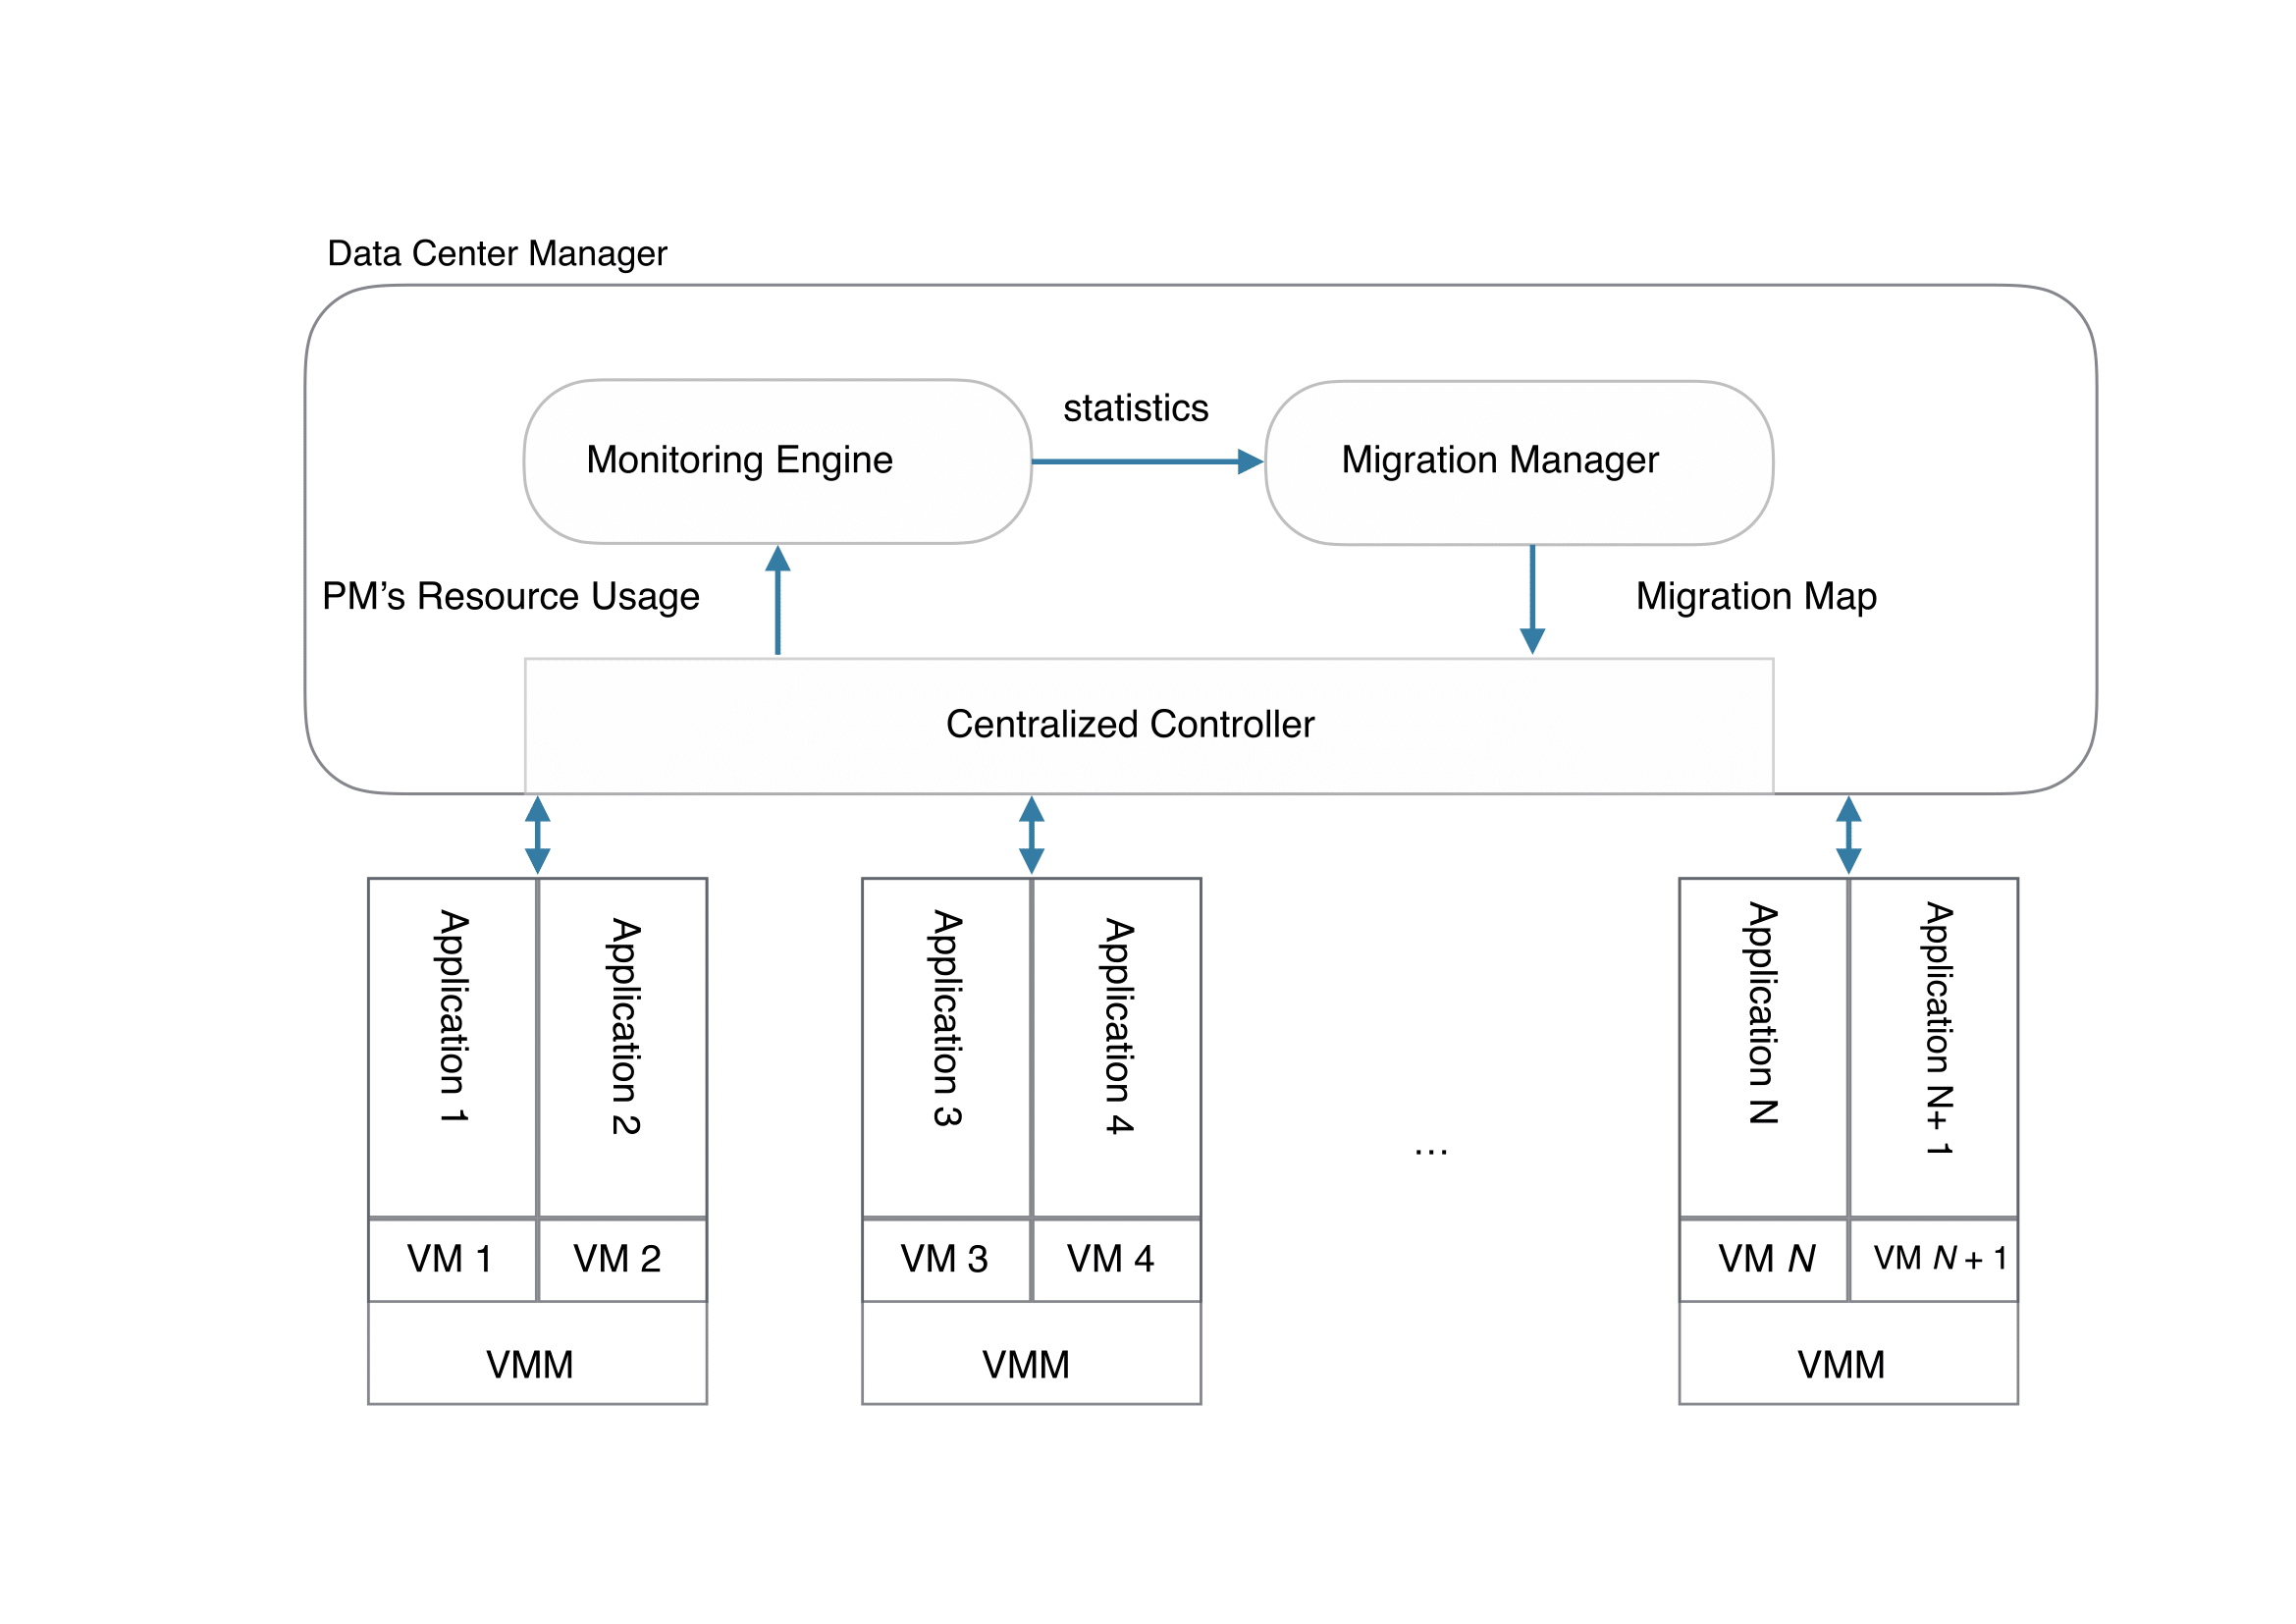
\includegraphics[width=1.0\textwidth]{pics/dataCenter-1.png}
% 	\caption{A datacenter management model \cite{Varasteh:2015fu}}
% 	\label{fig:arch}
% \end{figure}

% The taxonomy of server consolidation has not reach an agreement. In Verma's work \cite{Verma:2009wi}, they categorize it into three groups: static, semi-static and dynamic consolidation. In static consolidation, applications are placed on PM without any further movement. Semi-static refers to periodical adjustment. Dynamic consolidation is still applied on a set of VMs in response to their workload variations.









% A dynamic server consolidation approach
% can usually be decomposed into a series of steps, 
% reflecting the process required to produce a solution \cite{}. 
% These steps are shown in Figure \ref{} and discussed below:
% \begin{enumerate}
% 	\item When to migrate. Dynamic migration occurs on two scenarios: migrating VMs from overloaded server; and item migrating VMs from underloaded server.
% 	\item Which VMs to migrate.  After deciding to migrate a VM from a server, the next step is 
% 	to make a decision of which VM to migrate.
% 	\item Where to migrate the VMs. The key step is to determine where to allocate a VM which leads to global optimization.
% \end{enumerate}


% \subsection*{A Comparison between CaaS and IaaS based Cloud model}
% From a computing system design point of view, we believe service allocation and VM Placement
% are closely related and should be considered as a single allocation task.
% \subsection*{Service Allocation}
% Service allocation refers to the process of mapping a Web service on a certain type of VM.
% It is conducted by Cloud customers (e.g Web service providers) or Cloud brokers deligated by a 
% Cloud customer.
% The resource mapping involve with two steps, 
% resource demand profiling \cite{} and VM selection \cite{}. 
% Resource demand profiling is an estimation of the workload of a service. 
% Because the web application has dynamic workload over time \cite{}, 
% service providers or cloud brokers normally would like to estimate the future workload so that they 
% can choose how much resources to rent in order to guarantee the 
% Service Level Agreements (SLAs)  \cite{} to end customers. In this step, historical statistics
% are often used and based on its peak workload estimation, service providers often
% rent resources more than they need. Since the peak workload only accounts for a small portion
% of its total operation time, intelligent strategies are applied to tackle the over-provisioning and 
% under-provisioning problems.

% Public Cloud providers often provide various configurations of VM, 
% often refered to as VM types or instance types \cite{Li:2011ti}. 
% An instance type is defined as its resources such as memory size, number of processors and 
% CPU frequency. 

% Previous research focus on how to rent an appropriate amount of resources so that it minimize the 
% service providers' costs.

% Ref \cite{Candeia:2010wt} considers e-Science applications with bag-of-tasks (BoT) model. It
% aims at executing a bag of independent tasks with the least amount of Cloud resources before
% a deadline.
% Unlike a service allocation problem, where service is permanantly deployed in a reserved VM, 
% they consider an on-demand VM allocation. 
% That means, when a bag of tasks comes, the system
% dynamically assign a set of VM to execute these tasks. 
% It evaluates four heuristic algorithms and 
% concludes that a greedy-based approach achieves the best result.

% Li et al \cite{Li:2011ti} consider a dynamic cloud scheduling problem 
% from Cloud brokers' perspective. It considers scenarios such as Cloud provider changing its offer 
% (e.g changing of pricing schemes or VM types) and service performance changing, 
% a cloud broker needs to adjust the VMs allocation across multiple Cloud providers. 
% This work proposes a model which maximize a Cloud consumers' profit by adjusting VMs across
% multiple Clouds. Their model does not consider a Cloud provider's profit.

% Wang and Xia \cite{Wang:2016ui} propose a MIP formulation for energy-aware VM placement in Cloud.
% The major difference between their work and previous work is that they use a non-linear energy model \cite{Gandhi:2009wp}.  Based on this model, they consider two resources CPU and memory. In order to solve the non-linear problem, they propose a linearization method which uses piecewise linear function to approximate the non-linear objective function. In the end, they uses a relaxation method to relax the integer linear programming problem into continuous and apply a rounding function to obtain a near-optimal solution. In summary, the energy model is the key objective in consolidation problem. With different models, the applied algorithm can be very different. However, EC approaches can deal with both linear and non-linear problem without any changes. That is an obvious advantage. 

% Virtualization technology was first developed in IBM System/360 in 1960s 
% targeting a finer granularity resource management. 
% It partitions a physical machine into separated resources 
% called virtual machine (VM) which can be allocated 
% and moved from one server to another. 
% This flexibility not only allows resources to be managed in a dynamic manner, 
% but also enables server consolidation.

% In a Cloud datacenter, server consolidation is used as technique to combat \emph{server sprawl}.
% Server sprawl refers to the low utilization of physical servers. The main cause for server sprawl is
% the requirement of running applications in isolation \cite{Vogels:2008bg}. 
% That is, an application is deployed in one or more servers which 
% offer much more resources than it needs. 
% With full virtualization \cite{}, a server's physical resources including CPUs, memory, and I/O devices
% are divided into finer granularity level of resources.
% Virtual machines offer different sizes of resources that 
% can be choosed to satisfy different demands from applications. 

% \subsection*{An Overview of Evolutionary Computation}


% \subsection*{Initial Placement}

% \section*{Container-based VM Multiplexing}
% Container has been introduced back in the 1980s' \cite{}. The recent development of container
% allows only one process running in a container; this is revolutionary invention is called application
% container. It plays an important role in Cloud computing since it is lightweighted, easier to configure
% and enable finer adjustment than the VM-based resource management.


% \begin{figure}
% 	\centering
% 	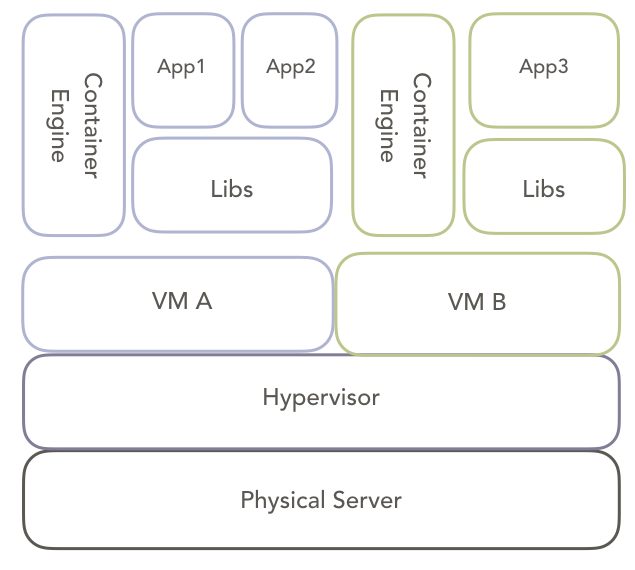
\includegraphics[width=0.6\textwidth]{pics/container.png}
% 	\caption{A Container as a Service Deployment Model}
% 	\label{fig:container}
% \end{figure}

% % % % % \section*{Dynamic VM Placement}
% % % % The traditional dynamic VM placement approaches can be categorized into three groups: Heuristic
% % % based approaches, deterministic approaches and dyanmic techniques with load prediction.

% % However, we believe the dynamic VM placement problem is highly dependent on an overall workload

% \section*{Large scale VM Placement}
% If you are writing an MSc or PhD thesis you should \emph{not} be using this style. Instead use \verb=vuwthesis=, which is based on the book style, and conforms to the VUW thesis rules. The thesis style is rather different from the project report style. 

% This document is formatted using a local (to ECS and MSOR at VUW) style file. When you write your project report you should be very careful when changing the beginning. The document class settings should read:

% \begin{verbatim}
% \documentclass[11pt
%               , a4paper
%               , twoside
%               , openright
%               ]{report}
% \end{verbatim}
% The options to the document class specify that:
% \begin{itemize}
% \item 11pt font is to be used for the main body text,
% \item  we will print on A4 paper, 
% \item we will use duplex (two-sided) printing,
% \item we want chapters to start on a right-hand page. 
% \end{itemize}

% The opitons you supply to the  \texttt{vuwproject} style will depend upon
% what you are using the style for.

% \subsection{Specifying the details}
% The \texttt{vuwproject} style sets up the front page properly, and provides various commands allowing you to specify the author, title, supervisor or supervisors, the school from which the report is being submitted and the degree that the report is being submitted for. The style has deliberately been designed to do as little as possible. This means that your document can easily be re-formatted as a technical report, or for submission to a conference or journal by using the appropriate style.

% It is also possible to use the style to easily produce documents on a
% stand-alone computer where your \LaTeX installtion might not have all
% of the  files and fonts available to machines within ECS or MSOR.

% Most of the options to the \texttt{vuwproject} style are currently a simple
% choice and there's a default that will make it obvious if you do not make
% a choice.

% Use one of the following options to use fonts available on ECS/MSOR machines
% or to use images that imitate them (assumes you have copies of the images)
% \begin{itemize}
% \item \verb+font+
% \item \verb+image+
% \end{itemize}

% Use one of the following options to set the school,
% \begin{itemize}
% \item \verb+ecs+
% \item \verb+msor+
% \end{itemize}

% Use one of the following options to choose a pre-defined degree,
% \begin{itemize}
% \item \verb+bschonscomp+
% \item \verb+mcompsci+
% \end{itemize}

% or use this command to use an explicit degree or diploma name
% \begin{itemize}
% \item \verb+\otherdegree{DEGREE OR DIPLOMA NAME}+
% \end{itemize}

% So, for example, to submit a report for the Master of Comp Sci degree, which
% the style knows about, from within ECS, using the images, you'ld ensure the
%  \texttt{vuwproject} line options looked like:

% \begin{verbatim}
% \usepackage[image,ecs,mcompsci]{vuwproject}
% \end{verbatim}

% whereas for a degree from within MSOR, when creating the final version on
% an ECS or MSOR machine where you have access to the fonts, you would use
% these options

% \begin{verbatim}
% \usepackage[font,msor]{vuwproject}
% \end{verbatim}


% and add the other degree's name using this command 

% \begin{verbatim}
% \otherdegree{DEGREE OR DIPLOMA NAME}
% \end{verbatim}

% To specify the supervisor or supervisors use either of the following commands in the preamble.
% \begin{itemize}
% \item \verb+\supervisor{The Supervisor}+
% \item \verb+\supervisors{Super 1 and Super 2}+
% \end{itemize}

% If you fail to set any degree or supervisor, or the school, then the front page will report this.

% The \texttt{vuwproject} style also sets the default font to be Palatino, using the \texttt{mathpazo} package. Palatino is one of VUW's `offical' fonts, and is the font used for the heading on the front page. The \texttt{mathpazo} package also typesets maths in a style which suits Palatino. 

% \section{Copying the style}
% If you want to write your project report away from VUW you will need to make your own copy of the \texttt{vuwproject} style.

% You can find out where the original lives by reading the messages that \LaTeX\ prints when it is run.

% Alternatively, you can down load a copy of the  \texttt{vuwproject} style from
% the ECS webpages.

% Any changes made to your own copy of the \texttt{vuwproject} style will not be reflected in the original, and \textit{vice versa}. Hence it makes sense to leave this as it is, and use a local style file for your own definitions.   

\chapter{Preliminary Work}\label{C:preliminary}
% \LaTeX\ is a very good tool for producing well-structured documents 
% carefully. It is very bad tool for banging things together in a rush 
% and panic. 

% \section{Floats}
% One perennial problem with \LaTeX\ is its treatment of 
% \emph{floats}.  Suppose you have a figure or table which you want to 
% include in your document. Where should it go? Traditional typesetting 
% practice is to put these in some convenient place, such as the top or 
% bottom of the current or next page, or at the end of the section or 
% chapter.  \LaTeX\ adopts a similar strategy, and allows floats to 
% ``float'' away from where they were defined. You can give a hint 
% about where you want the figure, but \LaTeX\ may move it. Sometimes 
% this is fine but sometimes you may want to have more control and 
% insist that a float goes \emph{here}. Anselm Lingau's 
% \textsf{float} package gives you this flexibility. For example, the following figure is an example of a non-floating float:

% \begin{fig}[H]
% \begin{center}
% \begin{tabular}{l|lll}
% $\delta$ & $\mathit{a}$ & $\mathit{b}$ & $\Lambda$ \\ \hline 
% $S_{1}$  & $\{\}$       & $\{\}$      & $\{S_{2}, S_{5}, S_{10}\}$\\
% $S_{2}$  & $\{S_{3}\}$  & $\{\}$      & $\{\}$\\
% $S_{3}$  & $\{S_{4}\}$  & $\{\}$      & $\{\}$\\
% $S_{4}$  & $\{S_{3}\}$  & $\{\}$      & $\{\}$\\
% $S_{5}$  & $\{\}$       & $\{S_{6}\}$ & $\{\}$\\
% $S_{6}$  & $\{\}$       & $\{S_{7}\}$ & $\{S_{8}\}$\\
% $S_{7}$  & $\{S_{6}\}$  & $\{\}$      & $\{\}$\\
% $S_{8}$  & $\{S_{9}\}$  & $\{\}$      & $\{\}$\\
% $S_{9}$  & $\{\}$       & $\{S_{8}\}$ & $\{\}$\\
% $S_{10}$ & $\{S_{11}\}$ & $\{\}$      & $\{\}$\\
% $S_{11}$ & $\{\}$       & $\{S_{10}\}$& $\{\}$\\ 
% \end{tabular}
% \caption{The transition function of an NFA with $\Lambda$  transitions}

% \end{center}
% \end{fig}

% On the other hand, Figure \ref{Fig:two} is a floating float. 



% \begin{fig}[tbh]
% \begin{center}
% \begin{tabular}{l|ll}
% $\delta''$ & $\mathit{a}$ & $\mathit{b}$ \\ \hline 
% $T_{1}$  & $T_{2}$ & $T_{3}$\\ 
% $T_{2}$  & $T_{4}$ & $T_{5}$\\ 
% $T_{3}$  & $T_{6}$ & $T_{7}$\\ 
% $T_{4}$  & $T_{8}$ & \\
% $T_{5}$  & $T_{10}$ & \\
% $T_{6}$  &  & $T_{11}$\\ 
% $T_{7}$  & $T_{3}$ & \\
% $T_{8}$  & $T_{4}$ & \\
% $T_{10}$  &  & $T_{5}$\\ 
% $T_{11}$  & $T_{6}$ & 
% \end{tabular}
% \caption{The transition function of an FA to accept 
% the same language.}
% \label{Fig:two}
% \end{center}
% \end{fig}

% You can define different types of new floats, and you can have tables 
% of them in the contents pages.


% \section{URL's}
% Use \verb=\url= from the \textsf{url} package to typeset URL's. Just 
% using \verb+\texttt+ or \verb+\tt+ does not work:

% \begin{itemize}
% \item \verb+\texttt{http://www.mcs.vuw.ac.nz/~neil/}+
% \item \verb+\url{http://www.mcs.vuw.ac.nz/~neil/}+
% \end{itemize}

% Give:
% \begin{itemize}
% \item \texttt{http://www.mcs.vuw.ac.nz/~neil/}
% \item \url{http://www.mcs.vuw.ac.nz/~neil/}
% \end{itemize}
% If you use the \textsf{hyperref} package then you can produce PDF 
% files with clickable hyperlinks using \verb=\url=.

% \section{Graphics and \LaTeX}
% \LaTeX\ offers rather poor support for the inclusion of graphics. 
% There are lots of ways to include pictorial material in \LaTeX, all 
% of which are deficient in some way or other. Look at \cite{GRM97GC} for a 
% description of them. If your document does need to have pictures in it 
% it is worth thinking about what is needed \emph{before} you generate 
% the pictures.

% \section{The bibliography}

% You should build up your bibliography as you go along.  Trying to get 
% the details of the bibliography correct at the end of the project is 
% hard work. Make sure that you record all the relevant details. Beware 
% that material on the internet is likely to change very rapidly. If you 
% are going to include material which is only available on the internet, 
% then you should probably include in the reference the date on which 
% you obtained the document.

% \section{Run \LaTeX, run}

% \LaTeX\ builds up information about your document for the table of 
% contents, references and so on at each run. This means that, for 
% example, the table 
% of contents is really the table of contents of the previous 
% compilation. You may need to run \LaTeX\ two or three times to let it 
% catch up with itself. If you have cross references within your 
% bibliography (for example two papers from the same collection, such 
% as \cite{Dum93a,Dum93b}) you may need to run 
% BibTeX more than once. 

% It is also possible that the table of contents file has garbage in 
% it, and will prevent the document from being compiled. This may 
% happen if you have had to abort compilation, due to a bug in the 
% source file. If this is the case then removing the \texttt{.toc} file 
% will usually solve the problem. You will have to fix the original 
% bug, of course.


% \section{Find out more by\ldots}
% You can find out more by:
% \begin{itemize}
% \item reading any one of a number of books, such as \cite{GMS94,Lam94}. The 
% VUW library has copies of these;
% \item visiting  the Comprehensive \TeX\ Archive Network (CTAN) at 
% \url{www.ctan.org};
% \item typing \texttt{latex} into Google.
% \end{itemize}

% It is \emph{highly unlikely} that you are the first person who ever 
% wanted to do what you want to do with \LaTeX. Therefore it is likely 
% that someone has already solved your problem: the real key to using  
% \LaTeX\ well is to make effective use of what other people have done.

% \section{Summary}
% In this chapter we explained some things about \LaTeX.



% Service Oriented Architecture (SOA) and Cloud computing have significantly reformed the software industry. SOA provides a decentralized application architecture which allows software composition and reuse in a large, global scale. Meanwhile, Cloud computing provides  a scalable, reliable, and flexible infrastructure to web services. 


% These advantages come from virtualization technology, which provides different level of isolation \cite{vm_technology}: workload-level and full virtualization. Container \cite{container} is one of the workload level virtualization which allows single-application workloads sharing operating system and physical resources such as CPU time and memory. Therefore, this technology improves the utilization of a single virtual machine. The full virtualization is used to partition physical machine into a number virtual machines (VMs) which enables VM migration. 

% As the dramatic increase of web services and cloud facilities, the management of resources has become a critical issue. 
% In recent years, as the power bill has become the largest fraction of the operating cost of Cloud facility \cite{Energy_6}, to reduce power consumption has become a paramount concern for Cloud service providers.
% In order to achieve that, a common approach is to re-allocate web services to a minimum number of physical machines (PMs) \cite{Energy_7}. 
% Therefore, idle computing servers are turned down or put into save mode. This optimization process, often called \textit{consolidation} involves with two levels of delivery mode, Software as a service (SaaS) and Infrastructure as a service (IaaS). Because of the complexity, consolidation tasks for IaaS and SaaS are often considered as separated tasks with different objectives. 
% For SaaS, the challenges concentrate on satisfying the Service Level Agreements (SLAs) with unpredictable requests using a minimum amount of resources. Whereas, for IaaS, the challenges are the VM migrations and 
% energy conservation.  

% There are extensive algorithms proposed for SaaS and IaaS levels of resource allocation \cite{Mazumdar20174, dubois2015autonomic}.
% Ref. \cite{Service_2} proposes a heuristic algorithm for service consolidation in a set of servers with minimizing costs while avoiding the overload of server and satisfying end-to-end response time constraints. 

% Ref. \cite{Energy_8} proposes two algorithms for energy efficient scheduling of VMs in Cloud, including an exact VM allocation algorithm which is an extended Bin-Packing approach, and a migration algorithm based on integer linear programming. 

% However, as the two levels of resource allocation are interact with each other, we believe they cannot be separated. They should be considered as one global optimization with multi-objectives from the perspectives of both service providers and cloud providers. Therefore, in this paper, we first propose a model for solving \textit{service resource allocation in Cloud (SRAC)}. Secondly, we propose a NSGA-II-based multi-objective algorithm with specifically designed operators to solve the problem. The two objectives are:

% \begin{enumerate}
%   \item propose a model for solving IaaS and SaaS resource allocation together
%   \item propose a NSGA-II-based algorithm to solve SRAC.
% \end{enumerate}


% The rest of the paper is organized as follows. Section \ref{sec:back} discusses the traditional 
% approaches for IaaS and SaaS and the power model for VM allocation. It will also introduce
% related works of evolutionary multi-objective optimization techniques. Section \ref{sec:problem} describes the 
% definition of the SRAC problem. Section \ref{sec:method} introduces the representation and genetic operators for SRAC problem. Section \ref{sec:exp} illustrates the experiment design, results and discussions. Section \ref{sec:con} draws a conclusion and discusses the future work.

% Copyright information

\section{Background}
\label{sec:back}
\subsection{Traditional approaches}
Ref. \cite{ga_saas} proposes a single-objective genetic algorithm to solve placement of service (SaaS) on physical machines. Their major contributions are three-fold. Firstly, they consider web services as a workflow and optimize the makespan of a workflow. Secondly, they design a representation to the problem. Thirdly, they do not only consider computing 
nodes, but storage nodes as well.

Ref. \cite{Service_1} develops a \textit{Resource-Allocation-Throughput (RAT)} model for web service allocation. The \textit{RAT model} mainly defines several important variables for an atomic service which represents a software component. Based on this model, firstly, an atomic service's throughput equals its coming rate if the resources of the allocated VM are not exhausted. Secondly, increasing the coming rate will also increase an atomic service's throughput until the allocated resource is exhausted. Thirdly, when the resource is exhausted, the throughput will not increase as request increasing. At this time, the virtual machine reaches its capacity. 

Anton Beloglazov et al.  \cite{Energy_Service_2} propose two algorithms for VM allocation. The first one is a bin-packing algorithm, called Modified Best Fit decreasing (MBFD) which is used when a new VM allocation request arrives. The second algorithm, named Minimization of Migration, is used to adjust the current VMs’ allocation according to the CPU utilization of a physical machine. Their experiments have shown that these methods lead to a substantial reduction of energy consumption in Cloud data centers.

\subsection{Power Model}

Shekhar's research \cite{Energy_1} is one of the earliest in energy aware consolidation for cloud computing. They conduct experiments of independent applications running in physical machines. They explain that CPU utilization and disk utilization are the key factors affecting the energy consumption. They also find that only consolidating services into the minimum number of physical machines does not necessarily achieve energy saving, because the service performance degradation leads to a longer execution time, which increases the energy consumption. 

Bohra \cite{Energy_3} develops an energy model to profile the power of a VM. They monitor the sub-components of a VM which includes: CPU, cache, disk, and DRAM and propose a linear model (Eq~\ref{eq:vmeter}). 
Total power consumption is a linear combination of the power consumption of CPU, cache, DRAM and disk. The parameters
$\alpha$ and $\beta$ are determined based on the observations of machine running CPU and IO intensive jobs. 
\begin{equation}
\label{eq:vmeter}
  P_{(total)} = \alpha P_{\{CPU, cache\}} + \beta P_{\{DRAM, disk\}}
\end{equation}
Although this model can achieve an average of 93\% of accuracy, it is hard to be employed in solving SRAC problem, for the lack of data.

Anton Beloglazov et al. \cite{Energy_Service_2} propose a comprehensive energy model for energy-aware resource allocation problem (Eq~\ref{eq:anton}). $P_{max}$ is the maximum power consumption when a virtual machine is fully utilized;
$k$ is the fraction of power consumed by the idle server (i.e. 70\%); and $u$ is the CPU utilization. This linear relationship between power consumption and CPU utilization is also observed by \cite{Energy_4, Energy_5}. 
\begin{equation}
\label{eq:anton}
  P(u) = k \cdot P_{max} + (1 - k) \cdot P_{max} \cdot u
\end{equation}


\subsection{Multi-objective Evolutionary Optimization}
A multi-objective optimization problem consists of multiple objective functions to be optimized.
A multi-objective optimization problem can be stated as follows:
\begin{align}
\min \ \ & \vec{f}(\vec{x}) = (f_1(\vec{x}), \dots, f_m(\vec{x})), \\
s.t. \ \ & \vec{x} \in \Omega.
\end{align}
where $\Omega$ stands for the feasible region of $\vec{x}$.

Multi-objective Evolutionary Optimization Algorithm (MOEA) are ideal for solving multi-objective optimization problems \cite{MOEA}, because MOEAs work with a population of solutions. With an emphasis on moving towards the true Pareto-optimal region, a MOEA algorithm can be used to find multiple Pareto-optimal solutions in one single simulation run \cite{ope}. Therefore, this project would employ MOEA approaches. This is also the first time to employ MOEAs technique for SRAC problem.

\section{Problem Description}
\label{sec:problem}
We consider the problem as a multi-objective problem with two potentially conflicting objectives, 
minimizing the overall cost of web services and minimizing the overall energy consumption of the used physical machines. 

To solve the SRAC problem, we model an atomic service as its request and requests' coming rate, also known as frequency. 


The request of an atomic service is modeled as two critical resources: 
CPU time $A = \{A_1, A_i, \dots, A_t \}$ and 
memory consumption $M = \{M_1, M_i, \dots, M_t \}$, 
for each request consumes a $A_i$ amount of CPU time 
and $M_i$ amount of memory. 
The coming rate is denoted as $R = \{R_1, R_i, \dots, R_t \}$. 
In real world scenario, the size and the number of a request are both variant 
which are unpredictable, therefore, this is one of the major challenges in Cloud resource allocation. 
In this paper, we use fixed coming rate extracted from a real world dataset to represent real world service requests. 
 
The cloud data center has a number of available physical machines which are modeled as
CPU time $PA = \{PA_1, PA_j, \dots, PA_p\}$ and memory
$PM = \{PM_1, PM_j, \dots, PM_p\}$. $PA_j$ denotes the CPU capacity of a physical machine 
and $PM_j$ denotes the size of memory. A physical machine can be partitioned or
 virtualized into a set of virtual machines; 
 each virtual machine has its 
 CPU time $VA = \{VA_1, VA_n, \dots, VA_v\}$ and 
 memory $VM = \{VM_1, VM_n, \dots, VM_v\}$. 


The decision variable of service allocation is defined as $X^i_n$. $X^i_n$
is a binary value (e.g. 0 and 1) denoting whether a
service $i$ is allocated on a virtual machine $n$.
The decision variable of virtual machine allocation is defined as $Y^n_j$. $Y^n_j$
is also binary denoting whether a
VM $n$ is allocated on a physical machine $j$.


 In this work, we consider homogeneous physical machine which means physical machines have the same size of CPU time and memory. 
 The utilization of a CPU of a virtual machine is denoted as $U = \{U_1, U_n, \dots, U_v\}$. 
 The utilization can be calculated by Eq.\ref{eq:util}.

\begin{equation}
\label{eq:util}
  U_n =
  \begin{cases} 
    \frac{\sum_{i = 1}^t R_i \cdot A_i \cdot X^i_n}{VA_n}, \text{If }  \frac{\sum_{i = 1}^t R_i \cdot A_i \cdot X^i_n}{VA_n} < 1 \\
    1   \quad\quad\quad\quad\quad\quad\quad ,\text{otherwise}
  \end{cases}
\end{equation}

The cost of a type of virtual machine is denoted as $C = \{C_1, C_n \dots, C_v\}$. 



In order to satisfy the performance requirement, Service providers often define Service Level Agreements (SLAs) to ensure the service quality. In this work, we define throughput as a SLA measurement \cite{SLA_metric}. 
Throughput denotes the number of requests that a service could successfully process in a period of time. According to \textit{RAT} model, the throughput is equal to the number of requests when the allocated resource is sufficient. 
Therefore, if a VM reaches its utilization limitation, it means that the services have been allocated exceedingly.
Therefore, all services in that VM suffer from 
performance degradation.


Then we define two objective functions as the total energy consumption and the total cost of virtual machines:

\begin{equation}
\label{eq:energy}
\begin{aligned}
& {\text{minimize}}\\
& Energy = \sum\limits_{j=1}^p (k \cdot V_{max} + (1 - k) \cdot V_{max} \cdot \sum^v\limits_{n=1} U_n \cdot Y^n_j)\\
\end{aligned}
\end{equation}

\begin{equation}
\label{eq:cost}
\begin{aligned}
& & & & & & & Cost = \sum\limits_{j=1}^p\sum\limits_{n=1}^v C_n \cdot Y^n_j
\end{aligned}
\end{equation}

\subsubsection{Hard constraint}
A virtual machine can be allocated on a physical machine if and 
only if the physical machine has enough available capacity on every resource.

\begin{equation} 
\label{eq:constraint}
\begin{aligned}
\sum\limits_{n=1}^v VM_n \cdot Y^n_j \leq PM_j\\
\sum\limits_{n=1}^v VA_n \cdot Y^n_j \leq PA_j
\end{aligned}
\end{equation}

\subsubsection{Soft constraint}
A service can be allocated on a virtual machine even if the 
virtual machine does not have enough available capacity on every resource, but the allocated services will suffer from a quality 
degradation.
% For the soft constraint, we define that exceeding numbers of atomic services can still
%  be packed into a virtual machine, 
%  but if the resource of a virtual machine has been used up, all the applications 
%  in that VM will suffer from a quality degradation.
\begin{equation}
\sum\limits_{i=1}^t M_i \cdot R_i \cdot X_i^n  \leq VM_n
\end{equation}

\section{Methods}
\label{sec:method}
As we have discussed, Multi-objective Evolutionary Algorithms are good at solving 
multi-objective problems and NSGA-II \cite{nsgaii} has shown his effective and efficiency. NSGA-II is a well-known MOEA that has been widely used
in many real-world optimization problems. 
In this paper we also adopt NSGA-II to solve the SRAC problem. 
We first propose a representation and then present a NSGA-II based algorithm with novel genetic operators.

\subsection{Chromosome Representation}
SRAC is a two-level bin-packing problem, in the first level, 
bins represent physical machines and items represent virtual machines. Whereas, in the second level, a virtual machine acts like a bin and web services are items. 
Therefore, we design the representation in two hierarchies, virtual machine level and physical machine level. 

\begin{figure*}
\centering
  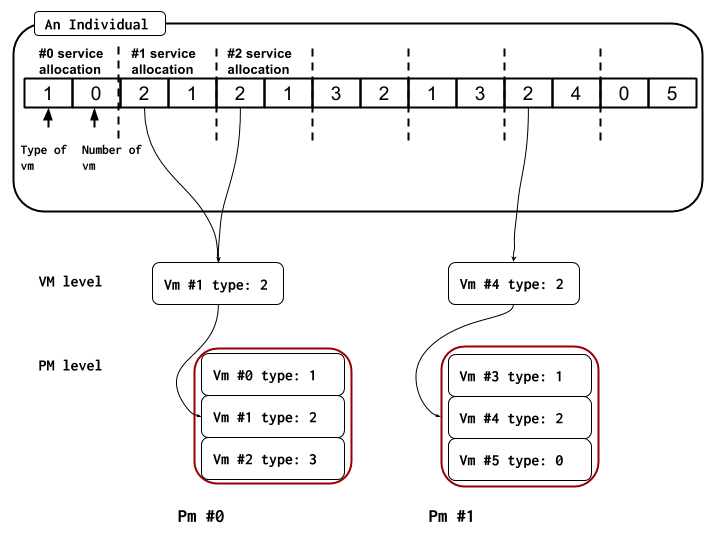
\includegraphics[width=0.8\textwidth]{pics/preliminary/cec.png}
  \caption{An example chromosome representation}
  \label{fig:rep}
\end{figure*}

Figure \ref{fig:rep} shows an example individual which contains seven service allocations. Each allocation of a service is represented as a pair where the index of each pair represents the number of web service. The first number indicates the type of virtual machine that the service is allocated in. The second number denotes the number of virtual machine.  For example, in Figure \ref{fig:rep}, service \#1 and service \#2 are both allocated in the virtual machine \#1 while service \#1 and service \#5 are allocated to different virtual machines sharing the same type.
The first hierarchy shows the virtual machine in which a service is allocated by defining VM type and number. 
Note that, the VM type and number are correlated once they are initialized. 
With this feature, the search procedure is narrowed down in the range of existing VMs which largely shrinks the search space.
The second hierarchy shows the relationship between a physical machine and its virtual machines, which are implicit. The physical machine is dynamically determined according to the virtual machines allocated on it. 
For example, in Figure ~\ref{fig:rep}, the virtual machines are 
sequentially packed into physical machines. The boundaries of PMs are calculated by adding up the resources of VMs until one of the resources researches the capacity of a PM. At the moment, no more VMs can be packed into the PM, then the boundary is determined.
% That is, we employ a simple heuristic method, 
% where the boundary of a physical machine is dynamically calculated. by adding up the virtual machines resources sequentially until a physical machine is full. 
The reason we designed this heuristic is because a physical machine is always fully used before launching another. Therefore, VM consolidation is inherently achieved.

Clearly, specifically designed operators are needed to manipulate chromosomes. Therefore, based on this representation, we further developed initialization, mutation, constraint handling and selection method.

\subsection{Initialization}
\begin{algorithm}[!htb]
 \caption{Initialization}
 \footnotesize
 \textbf{Inputs:} \\
  VM CPU Time $VA$ and memory $VM$, \\
  Service CPU Time $A$ and memory $M$ \\
  consolidation factor c \\
 \textbf{Outputs:}
  A population of allocation of services

 \begin{algorithmic}[1]
  \FOR{ Each service $t$ }
    \STATE{ Find its most suitable VM Type}
    \STATE{ Randomly generate a VM type $vmType$ which is equal
            or better than its most suitable type}
    \IF { There are existing VMs with $vmType$}
      \STATE randomly generate a number $u$
      \IF{ $u <$ consolidation factor }
      \STATE randomly choose one existing VM with $vmType$ to allocate
      \ELSE
      \STATE launch a new VM with $vmType$
      \ENDIF
    \ELSE
      \STATE Create a new VM with its most suitable VM type
    \ENDIF

  \ENDFOR
 \end{algorithmic}
 \label{alg:init}
\end{algorithm}


The initialization (see Alg~\ref{alg:init}) is designed to generate a diverse population.
In the first step, for each service, it is able to find the most suitable VM type which is just capable of running the service based on its resource requirements. 
In the second step, based on the suitable VM type, a stronger type is randomly generated. If there exists a VM with that type, the service is either deployed in the 
existing VM or launch a new VM. We design a consolidation factor $c$ which is a real number manually selected from 0 to 1 to control this selection. If a
random number $u$ is smaller than $c$, the service is consolidated in an existing VM.

This design could adjust the consolidation, therefore, controls the utilization of VM.

\subsection{Mutation}
\begin{figure}
\centering
  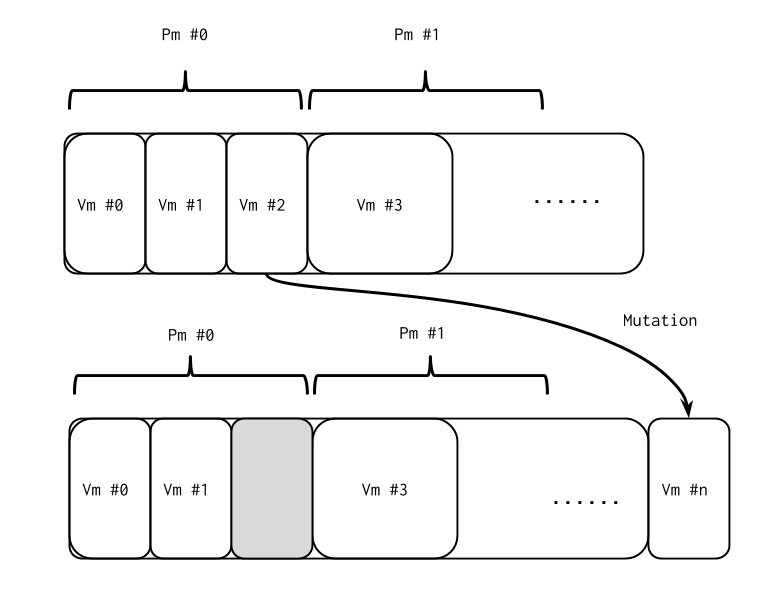
\includegraphics[width=0.7\textwidth]{pics/preliminary/hollow.png}
  \caption{An example mutation without insertion that causes a lower resource utilization}
  \label{fig:hollow}
\end{figure}

The design principle for mutation operator is to enable individuals exploring the entire feasible search space.
Therefore, a good mutation operator has two significant features, the exploration ability and the its ability to keep an individual within the feasible regions. In order to achieve these two goals, firstly, we generate a random virtual machine type which has a greater capacity than the service needs. It ensures the feasible of solutions as well as exploration capability. Then, we consider whether a service is consolidated with the consolidation factor $c$. 

The consolidation is conducted with a roulette wheel method which assigns fitness value to each VM according to the reciprocal of its current utilization. 
The higher the utilization, the lower the fitness value
it is assigned. 
Therefore, a lower utilization VM has a greater probability to be chosen. 
At last, if a new VM is launched, it will not be placed at the end of VM lists. Instead, it will be placed at a random position among the VMs. The reason is illustrated in Figure \ref{fig:hollow}. In the example, VM \#2 is mutated into a new type and be placed at the end of the VM list. However, because of the size of VM \#3 is too large for PM \#0, the hollow in PM \#0 will never be filled. This problem can be solved with the random insertion method.
\begin{algorithm}[!htb]
 \caption{Mutation}
 \footnotesize
 \textbf{Inputs:} \\
  An individual
  VM CPU Time $VA$ and memory $VM$, \\
  Service CPU Time $A$ and memory $M$ \\
  consolidation factor c \\
 \textbf{Outputs:}
  A mutated individual

 \begin{algorithmic}[1]
  \FOR{ Each service}
    \STATE Randomly generate a number $u$
    \IF { $u <$ mutation rate}
      \STATE find the most suitable VM Type for this service
      \STATE Randomly generate a number $k$
      \IF{ $k <$ consolidation factor }
        \STATE calculate the utilization of used VMs
        \STATE assign each VM with a fitness value of 1 / utilization and generate a roulette wheel
            according to their fitness values
        \STATE Randomly generate a number $p$, select the VM according to $p$
        \STATE Allocate the service
      \ELSE
        \STATE launch a new VM with the most suitable VM Type
        \STATE insert the new VM in a randomly choose position
      \ENDIF
    \ENDIF
  \ENDFOR
 \end{algorithmic}
 \label{alg:mutation}
\end{algorithm}

\subsection{Violation control method}
A modified violation ranking is proposed to deal with the soft constraint, for the hard constraint is automatically eliminated by the chromosome representation.
We define a violation number as the number of services which are allocated in the degraded VMs. 
That is, if there are excessive services allocated in a VM, then all the services are suffered from a degraded in performance. 
The violation number is used in the selection procedure, 
where the individuals with less violations are always preferred.

\subsection{Selection}
Our design uses the binary tournament selection with a constrained-domination principle. A constrained-domination principle is defined as following. A solution $I$ is considered constraint-dominate a solution $J$, if any of the following condition is true:
\begin{enumerate}
  \item Solution $I$ is feasible, solution is not,
  \item Both solutions are infeasible, $I$ has smaller overall
violations,
  \item Both solutions are feasible, solution $I$ dominates solution $J$.
\end{enumerate}

An individual with no or less violation is always selected. This method has been proved effective in the original NSGA-II paper \cite{nsgaii}.

\subsection{Fitness Function}
The cost fitness (Eq.\ref{eq:cost}) is determined by the type of VMs at which web service are allocated. 
The energy fitness is shown in Eq.\ref{eq:energy}, the utilizations (Eq.\ref{eq:util}) of VM are firstly converted into the utilizations of PM according to the proportion of VMs’ and PM’s CPU capacity.

\subsection{Algorithm}
The main difference between our approach and the original NSGA-II is that our approach has no crossover operator.

That is, a random switch of chromosome would completely destroy the order of VMs, 
hence, no useful information will be preserved. 
Therefore, we only apply mutation as the exploration method. Then, the algorithm becomes a parallel optimization without much interaction between its offspring, which is often addressed as Evolutionary Strategy \cite{evo_str}.
\begin{algorithm}[!htb]
 \caption{NSGA-II for SRAC}
 \footnotesize
 \textbf{Inputs:} \\
  VM CPU Time $VA$ and memory $VM$, \\
  PM CPU Time $PA$ and memory $PM$, \\
  Service CPU Time $A$ and memory $M$ \\
  consolidation factor c \\
 \textbf{Outputs:}
  A Non-dominated Set of solutions

 \begin{algorithmic}[1]
  \STATE Initialize a population $P$
  \WHILE{ Termination Condition is not meet}
    \FOR{ Each individual }
      \STATE Evaluate the fitness values
      \STATE Calculate the violation
    \ENDFOR

    \STATE non-Dominated Sorting of $P$
    \STATE calculate crowding distance
    \WHILE{ child number is less than population size }
      \STATE Selection
      \STATE Mutation
      \STATE add the child in a new population U
    \ENDWHILE
    \STATE Combine $P$ and $U$ \COMMENT{ for elitism}
    \STATE Evaluate the combined $P$ and $U$
    \STATE Non-dominated sorting and crowding distance for combined population
    \STATE Include the top popSize ranking individuals to the next generation

  \ENDWHILE
 \end{algorithmic}
 \label{alg:NSGAII}
\end{algorithm}

\section{Experiment}
\label{sec:exp}
\subsection{Dataset and Problem Design}
This project is based on both real-world datasets \textit{WS-Dream} \cite{Service_dataset} and simulated datasets \cite{Energy_9}. 
The \textit{WS-Dream} contains web service related datasets including network latency and service frequency (request coming rate). In this project, we mainly use the service frequency matrix. For the cost model, we only consider the rental of virtual machines with fixed fees (monthly rent). The configurations of VMs are shown in Table~\ref{tab:vm}, the CPU time and memory were selected manually and cost were selected proportional to their CPU capacity. The maximum PM's CPU and memory are set to 3000 and 8000 respectively. The energy consumption is set to 220W according to \cite{Energy_9}.

We designed six problems shown in Table \ref{tab:problem}, listed with increasing size and difficulty, which are used as representative samples of SRAC problem.

\begin{table}[]
\centering
\caption{Problem Settings}
\label{tab:problem}
\begin{tabular}{ccccccc}
\hline 

Problem           & 1  & 2  & 3  & 4  & 5   & 6    \\
Number of services & 20 & 40 & 60 & 80 & 100 & 200 \\ \hline
\end{tabular}
\end{table}

\begin{table}[]
\centering
\caption{VM configurations}
\label{tab:vm}
\begin{tabular}{@{}cccc@{}}
\toprule
VM Type & CPU Time & Memory & Cost \\ \midrule
1       & 250      & 500    & 25 \\
2       & 500      & 1000   & 50 \\
3       & 1500     & 2500   & 150\\
4       & 3000     & 4000   & 300\\ \bottomrule
\end{tabular}
\end{table}
\begin{flushleft}Selection Method with violation Control vs. without violation control\end{flushleft}
\begin{figure}
   \centering
   \begin{subfigure}[b]{0.45\textwidth} 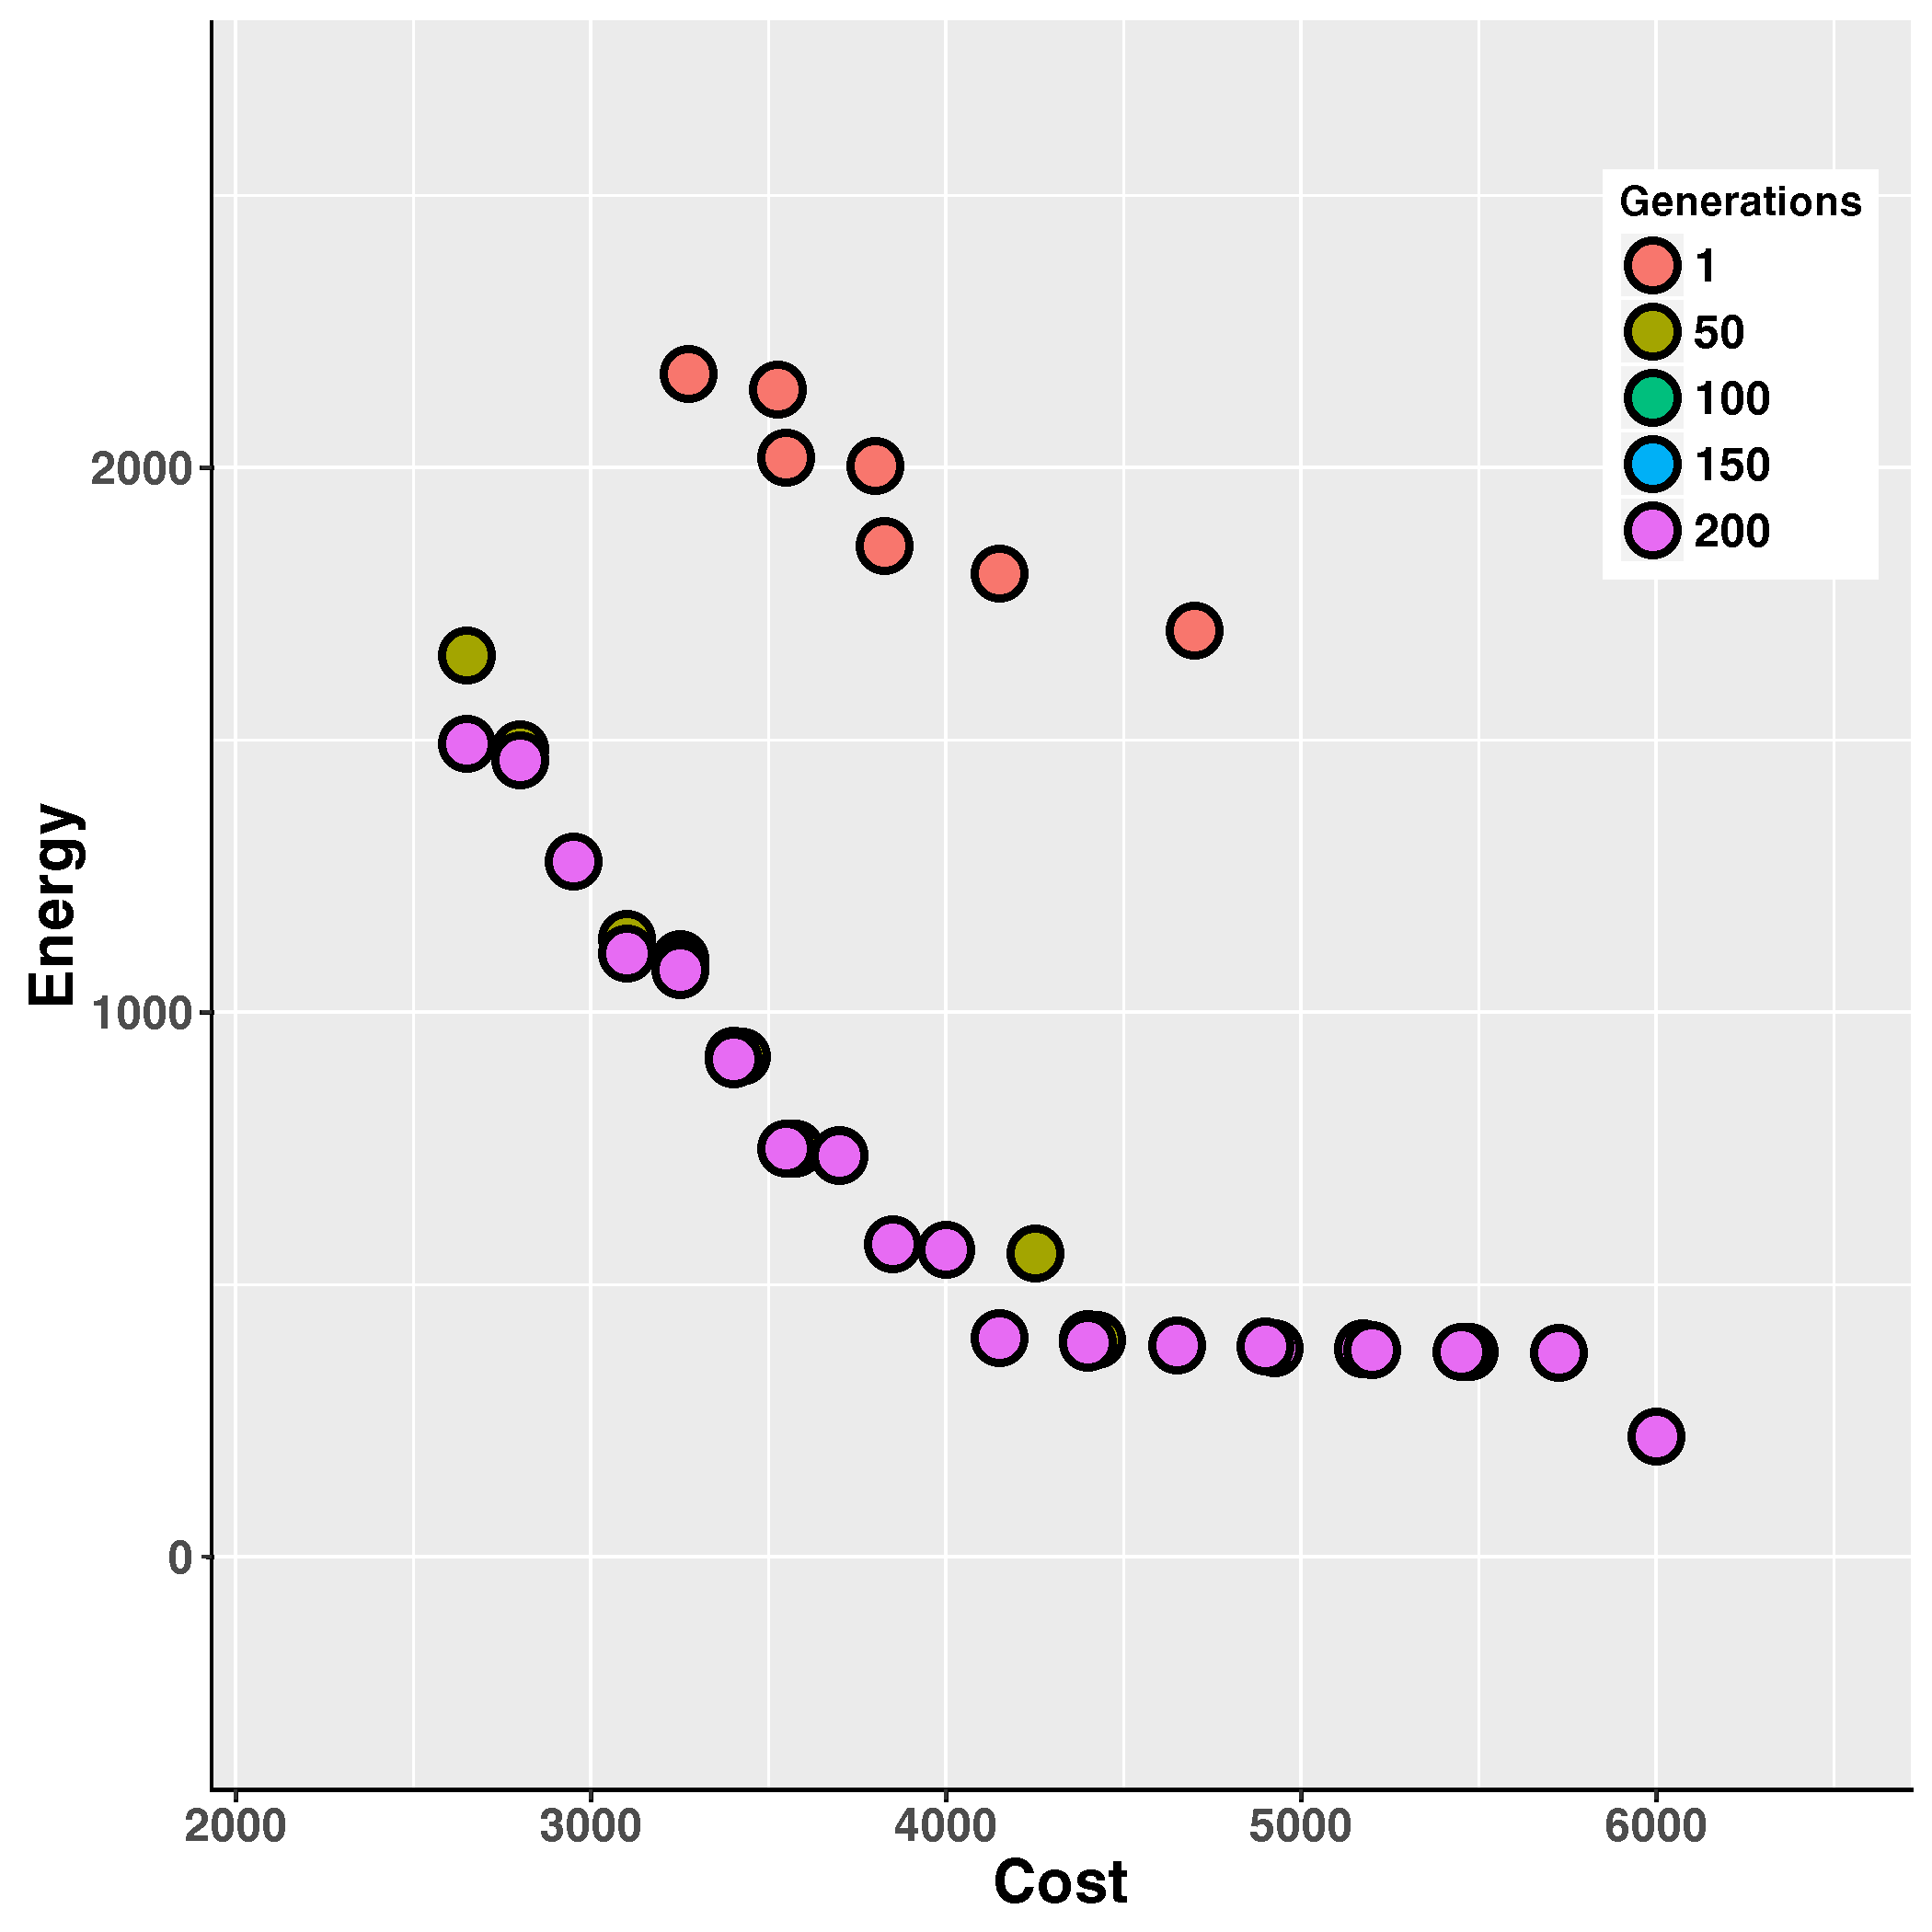
\includegraphics[width=\textwidth]{pics/preliminary/without/testCase1_.png}
   \caption{Problem 1}
   \label{fig:a}
   \end{subfigure}
   \begin{subfigure}[b]{0.45\textwidth} 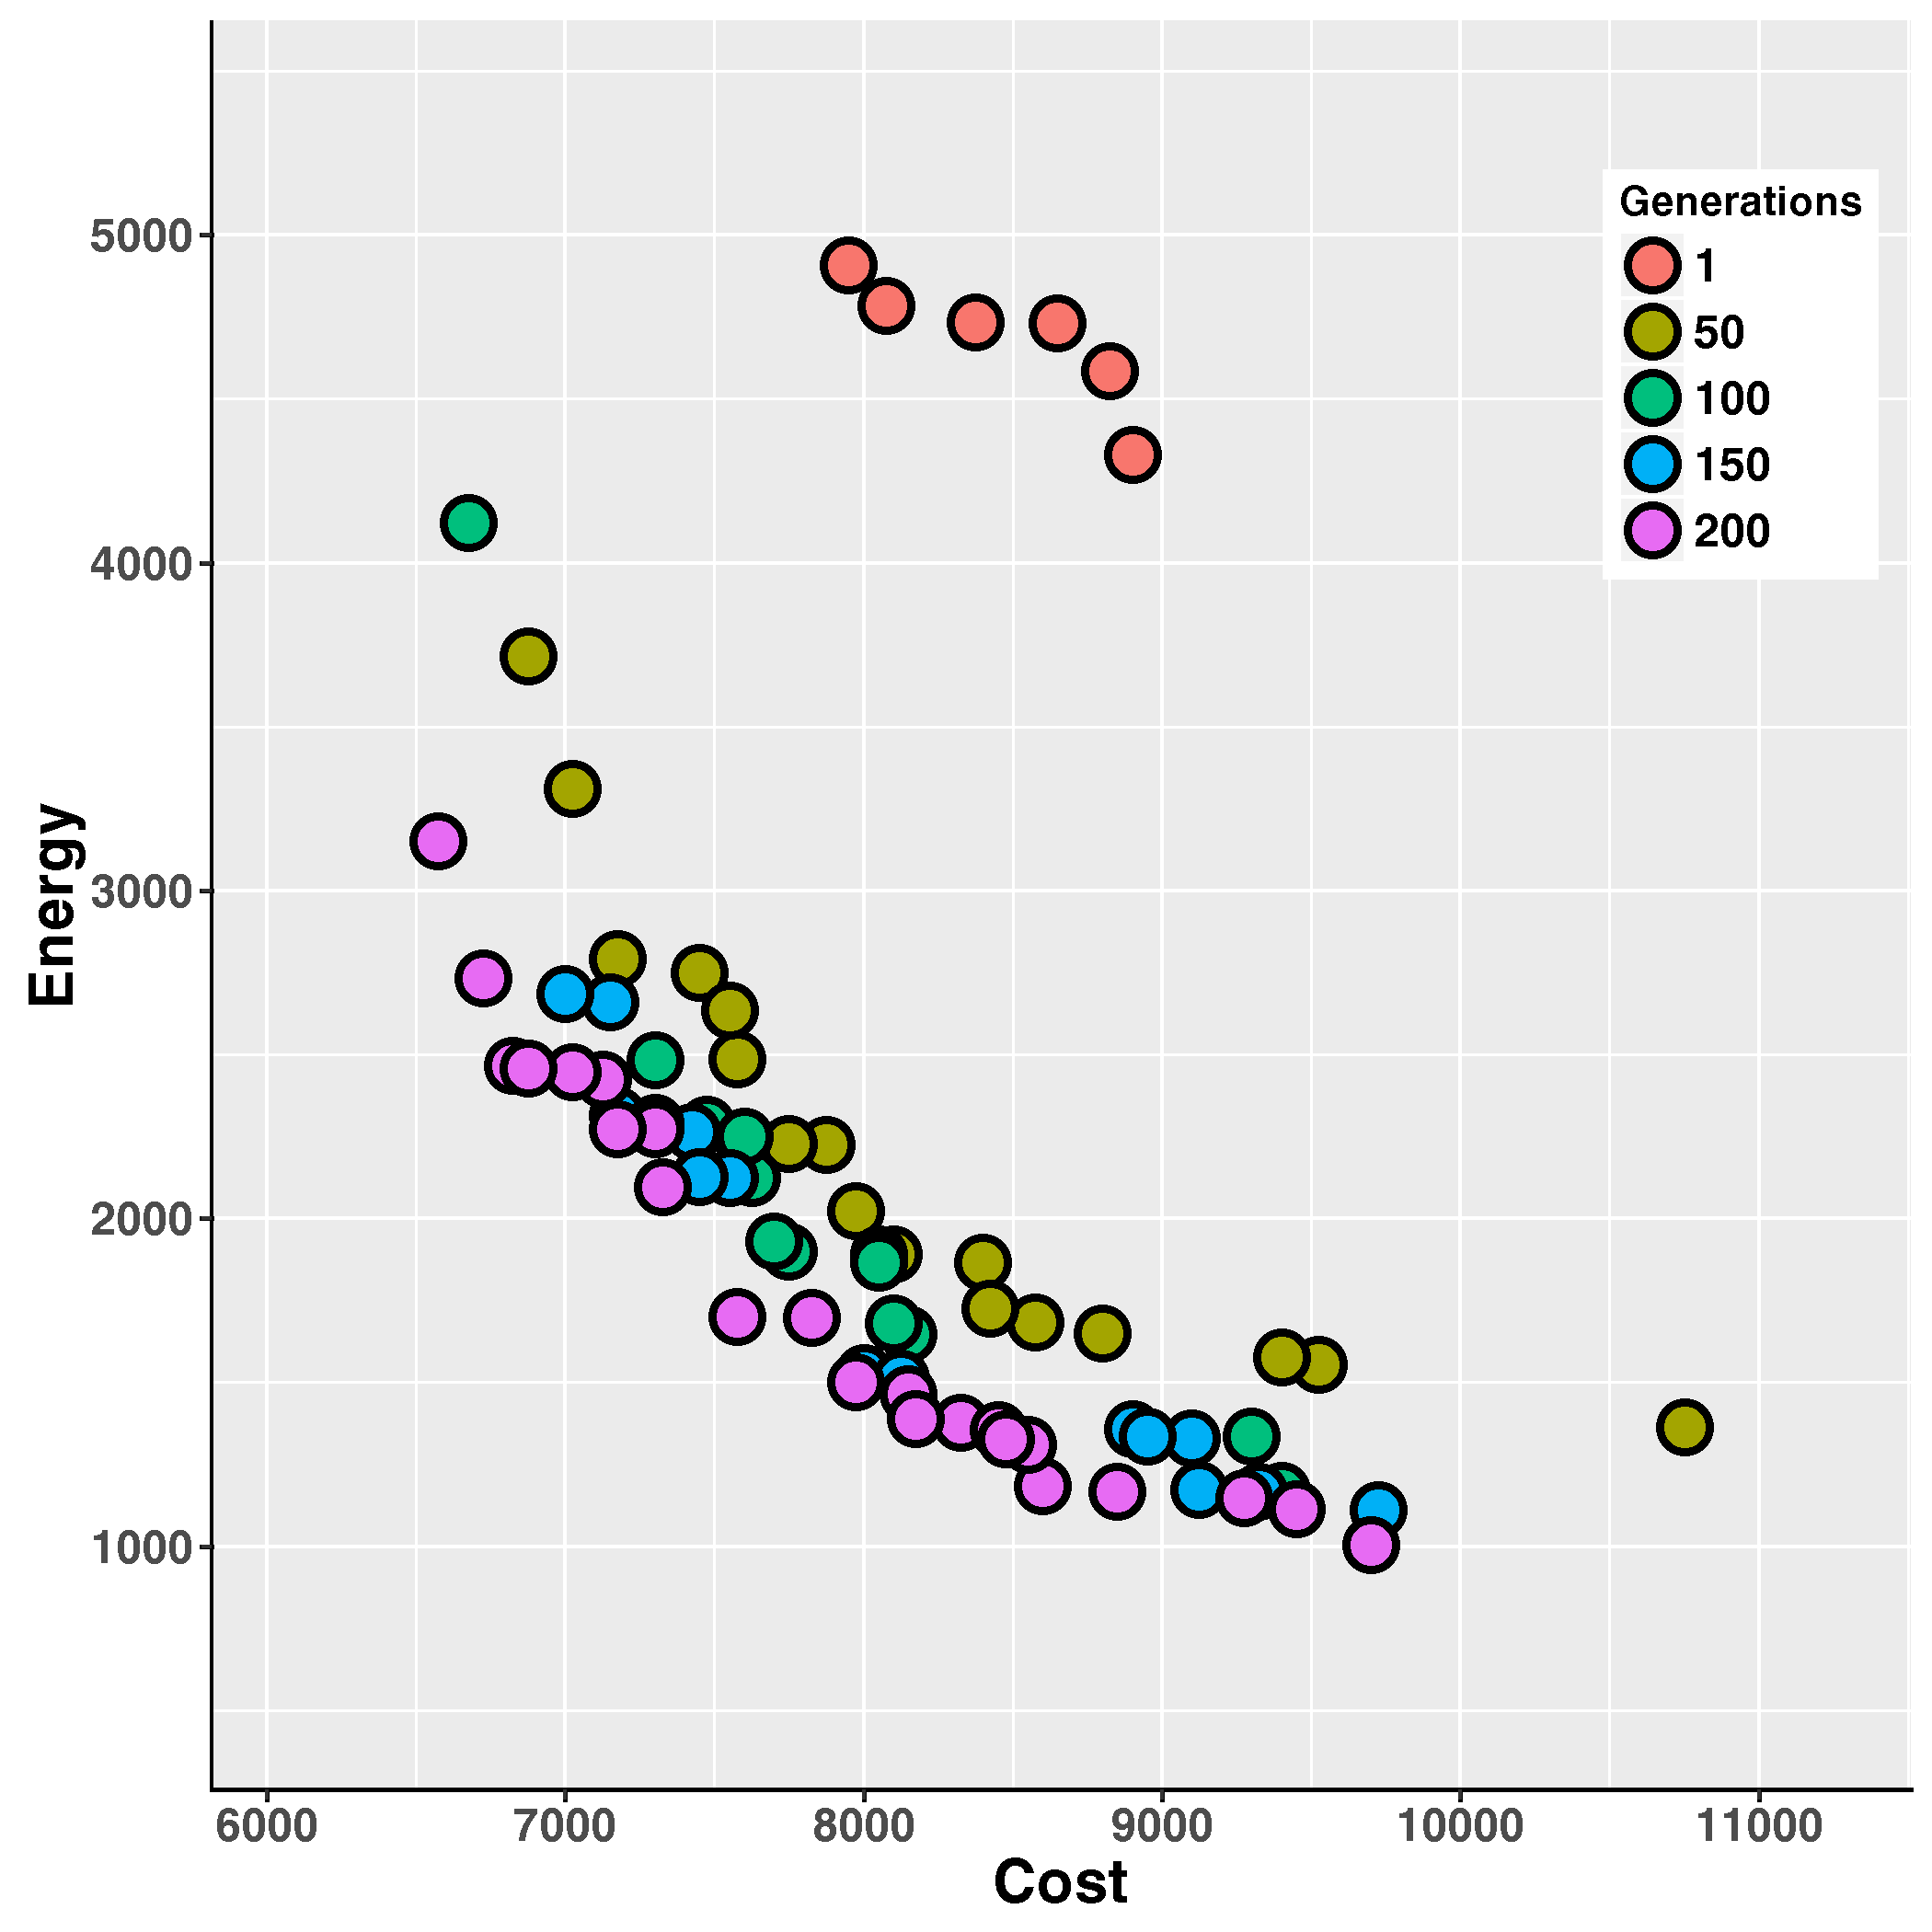
\includegraphics[width=\textwidth]{pics/preliminary/without/testCase2_.png}
   \caption{Problem 2}
   \label{fig:b}
   \end{subfigure}
   \begin{subfigure}[b]{0.45\textwidth}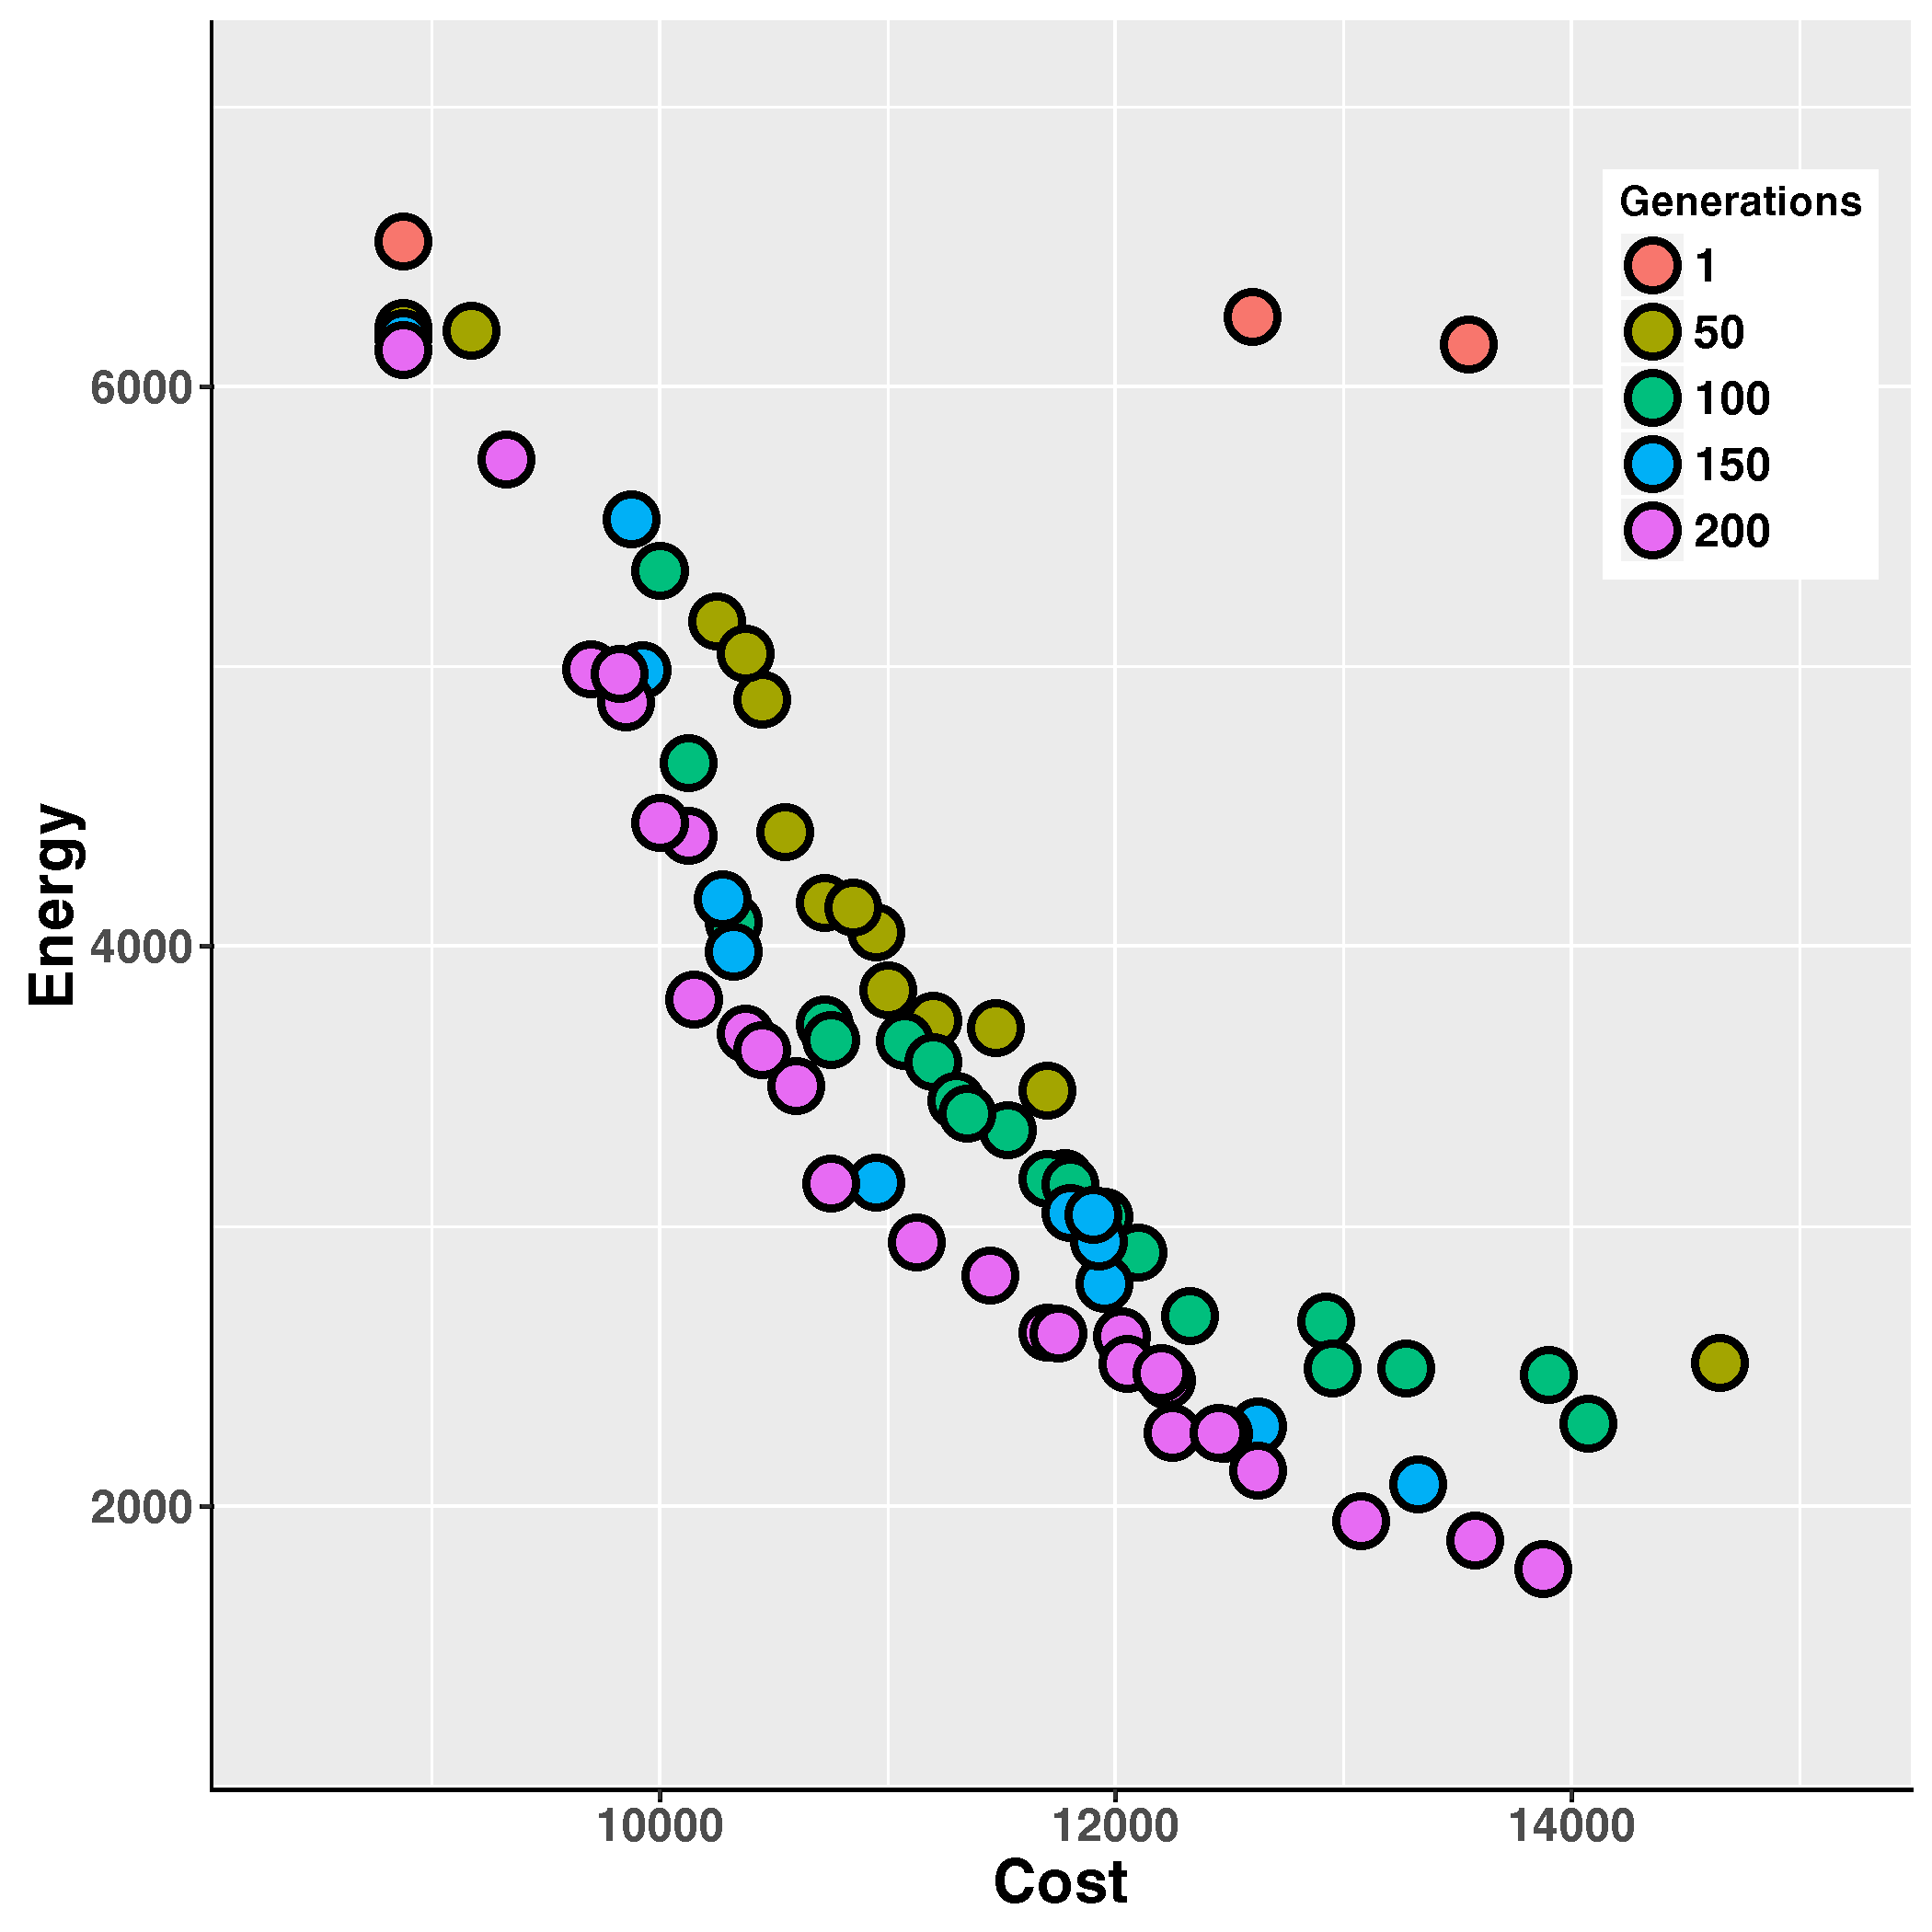
\includegraphics[width=\textwidth]{pics/preliminary/without/testCase3_.png}
   \caption{Problem 3}
   \label{fig:c}
   \end{subfigure}
   \begin{subfigure}[b]{0.45\textwidth}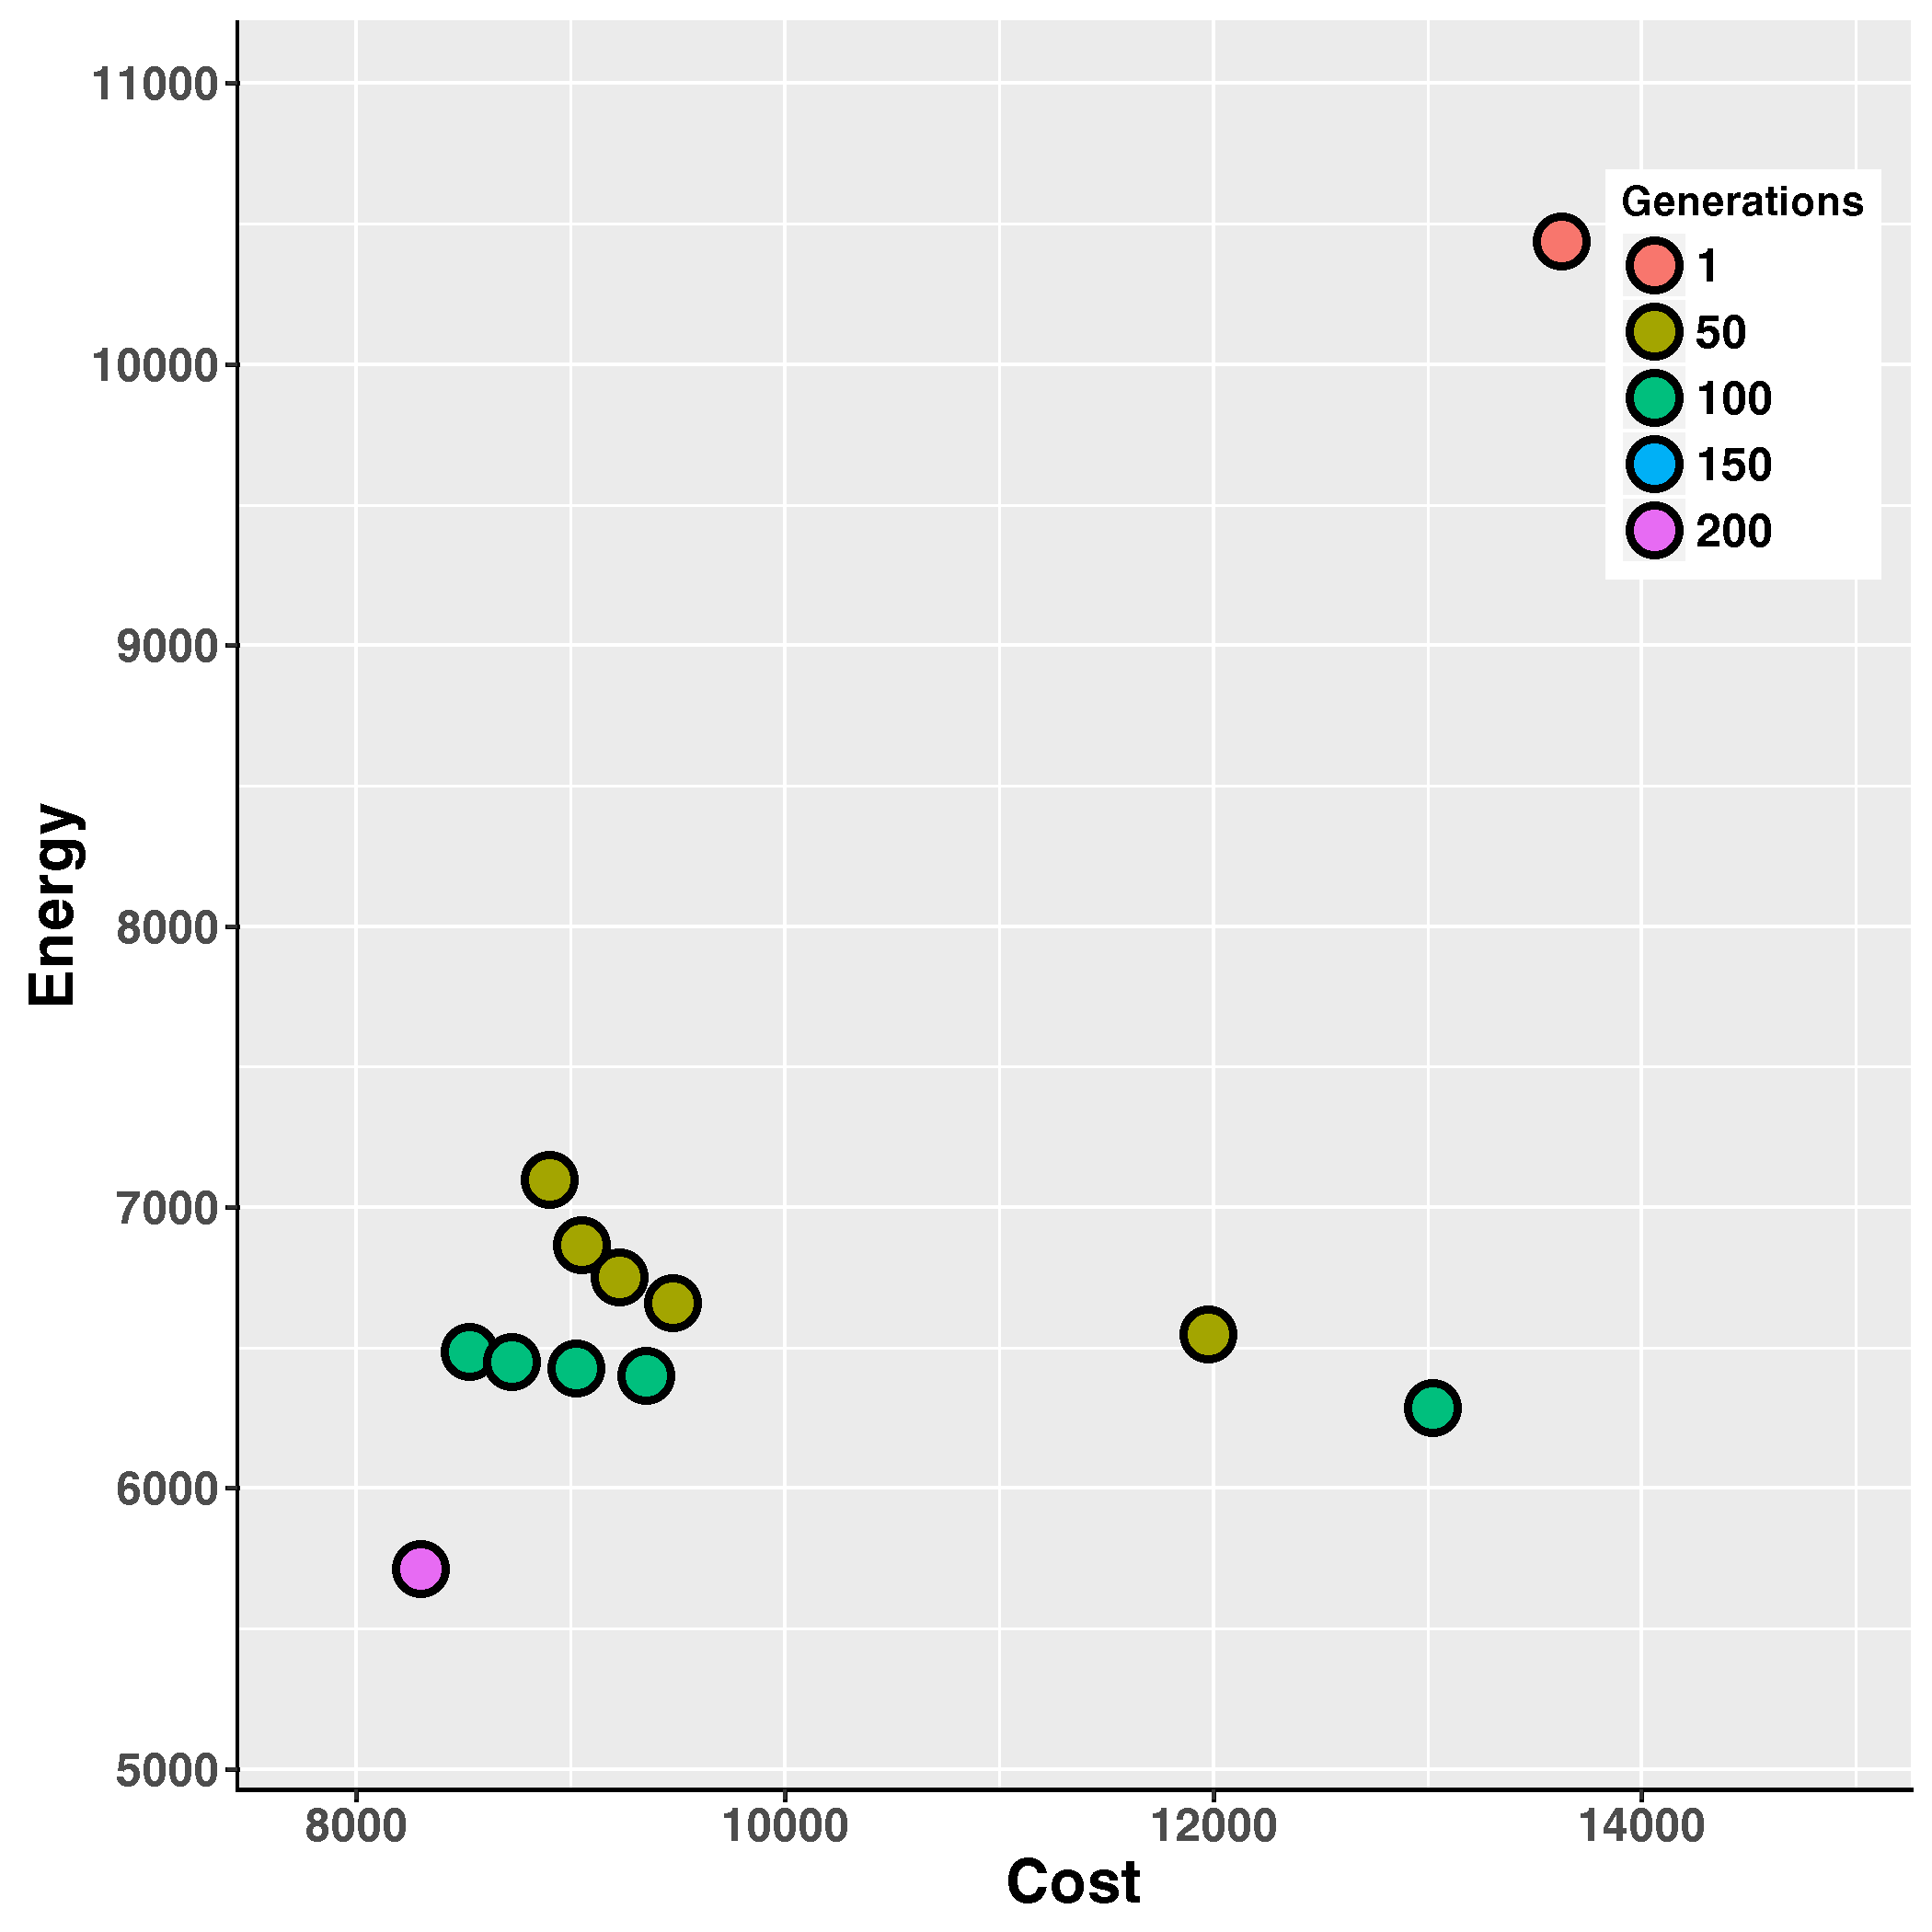
\includegraphics[width=\textwidth]{pics/preliminary/without/testCase4_.png}
   \caption{Problem 4}
   \label{fig:d}
   \end{subfigure}
   \begin{subfigure}[b]{0.45\textwidth}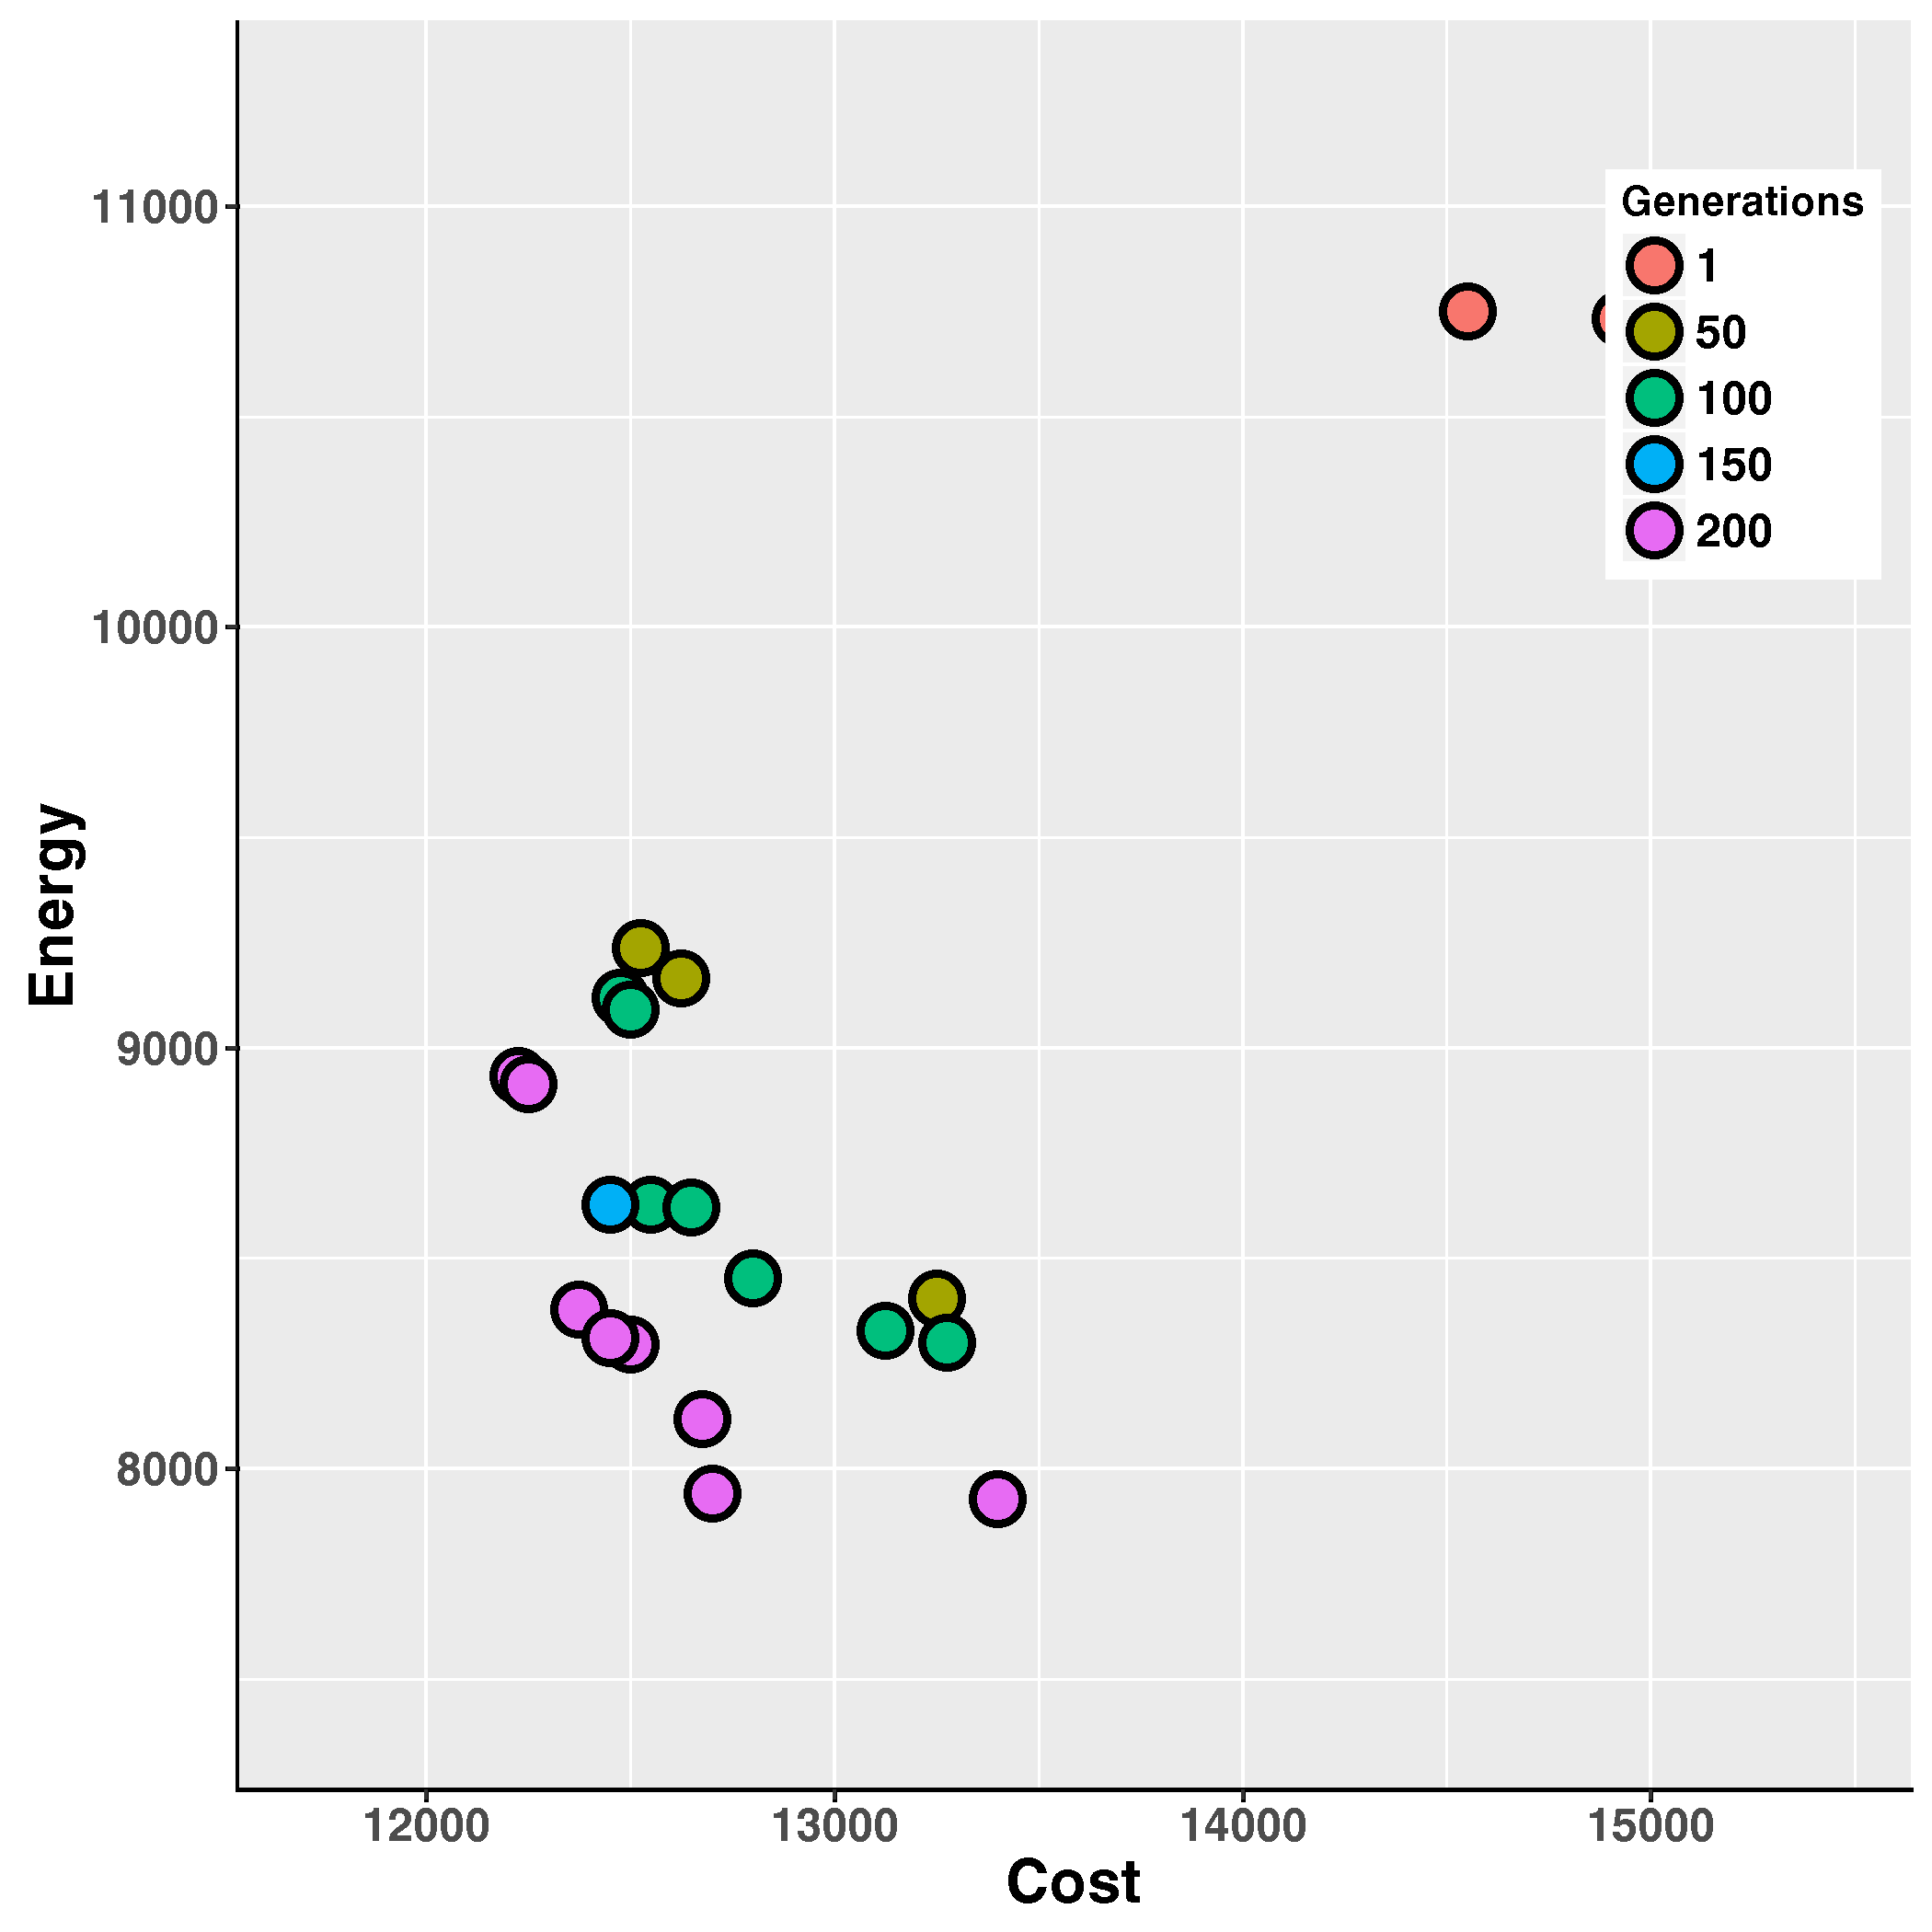
\includegraphics[width=\textwidth]{pics/preliminary/without/testCase5_.png}
   \caption{Problem 5}
   \label{fig:e}
   \end{subfigure}
   \begin{subfigure}[b]{0.45\textwidth}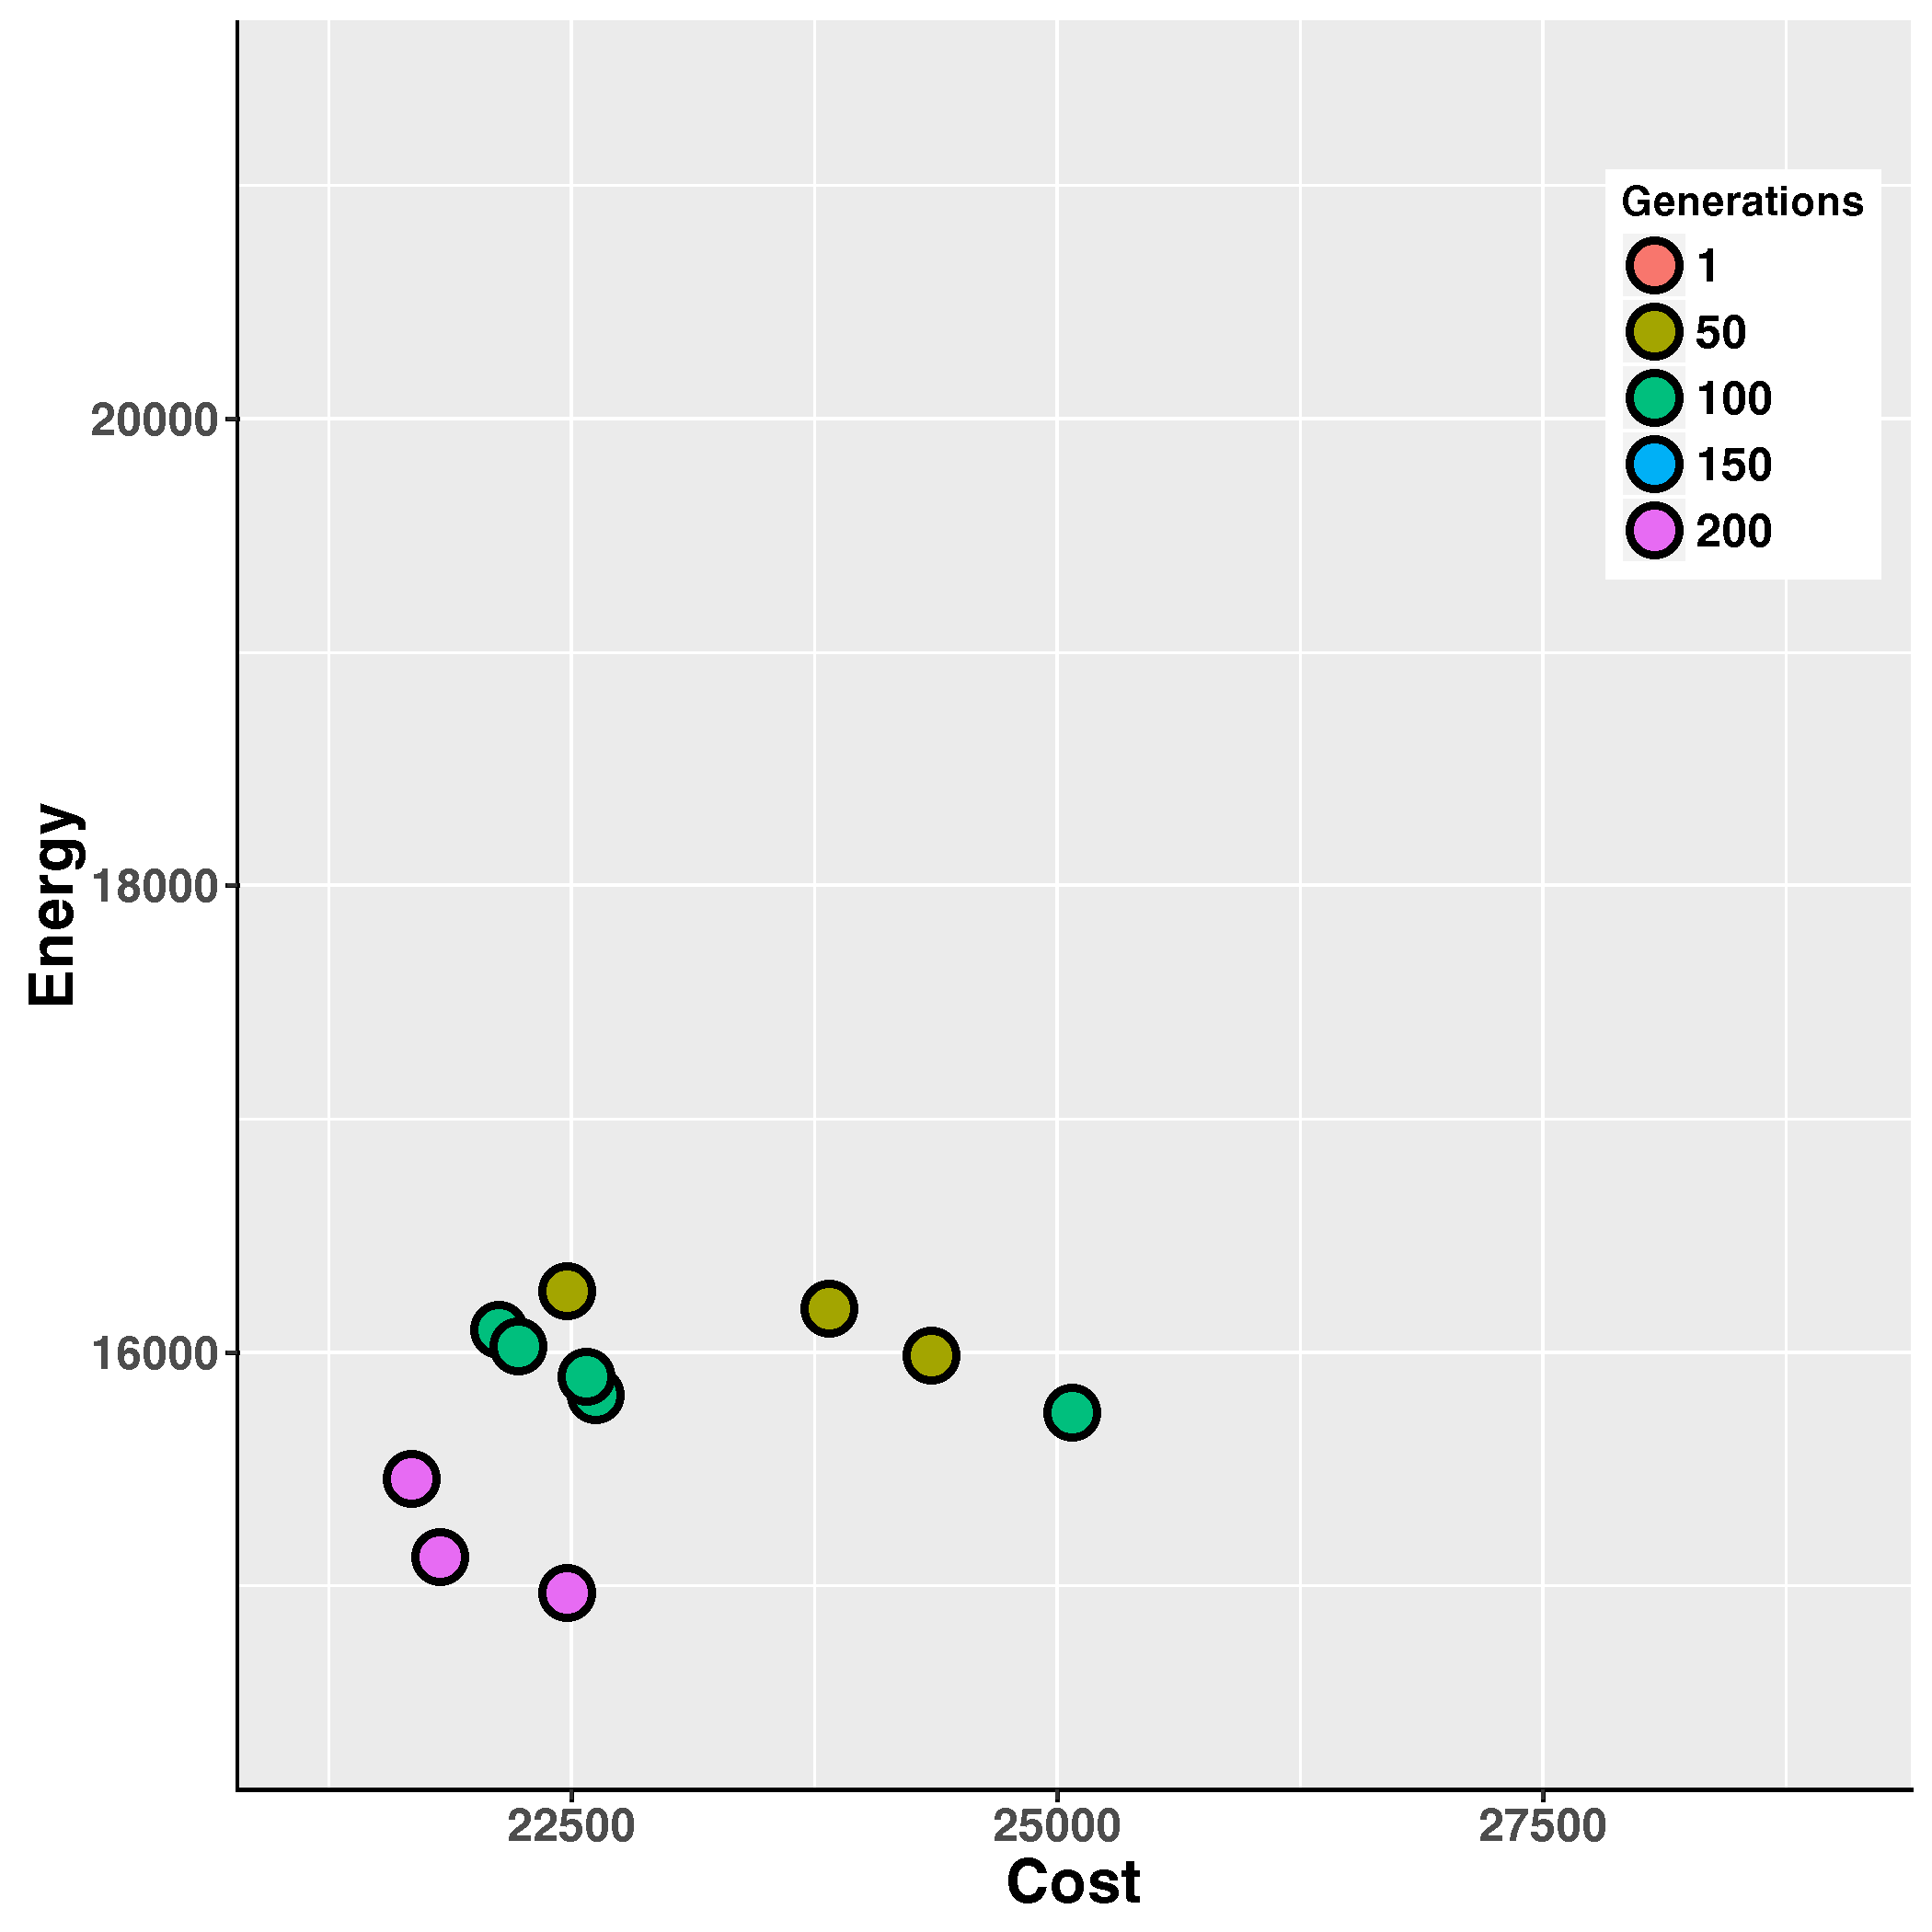
\includegraphics[width=\textwidth]{pics/preliminary/without/testCase6_.png}
   \caption{Problem 6}
   \label{fig:f}
   \end{subfigure}
   \caption{Non-dominated solutions evolve along with the generation}
   \label{fig:evolve}
\end{figure}

We conducted two comparison experiments. For the first experiment, we make a comparison between NSGA-II with violation control and NSGA-II without violation control. 
In second experiment, two mutation operators are compared. The first is the roulette wheel mutation, the second is the mutation with greedy algorithm. The mutation with greedy algorithm is a variant of roulette wheel mutation. The only difference is that instead of selecting a VM to consolidate with fitness values, it
always selects the VM with the lowest CPU utilization. 
Therefore, it is a greedy method embedded in the mutation.


The experiments were conducted on a personal laptop with 2.3GHz CPU and 8.0 GB
RAM. For each approach, 30 independent runs are performed for each problem with
constant population size 100. The maximum number of iteration is 200. $k$ equals 0.7. 
We set mutation rate and consolidation factor to 0.9 and 0.01.


\subsection{Results}
\begin{figure}
   \centering
   \begin{subfigure}[b]{0.45\textwidth}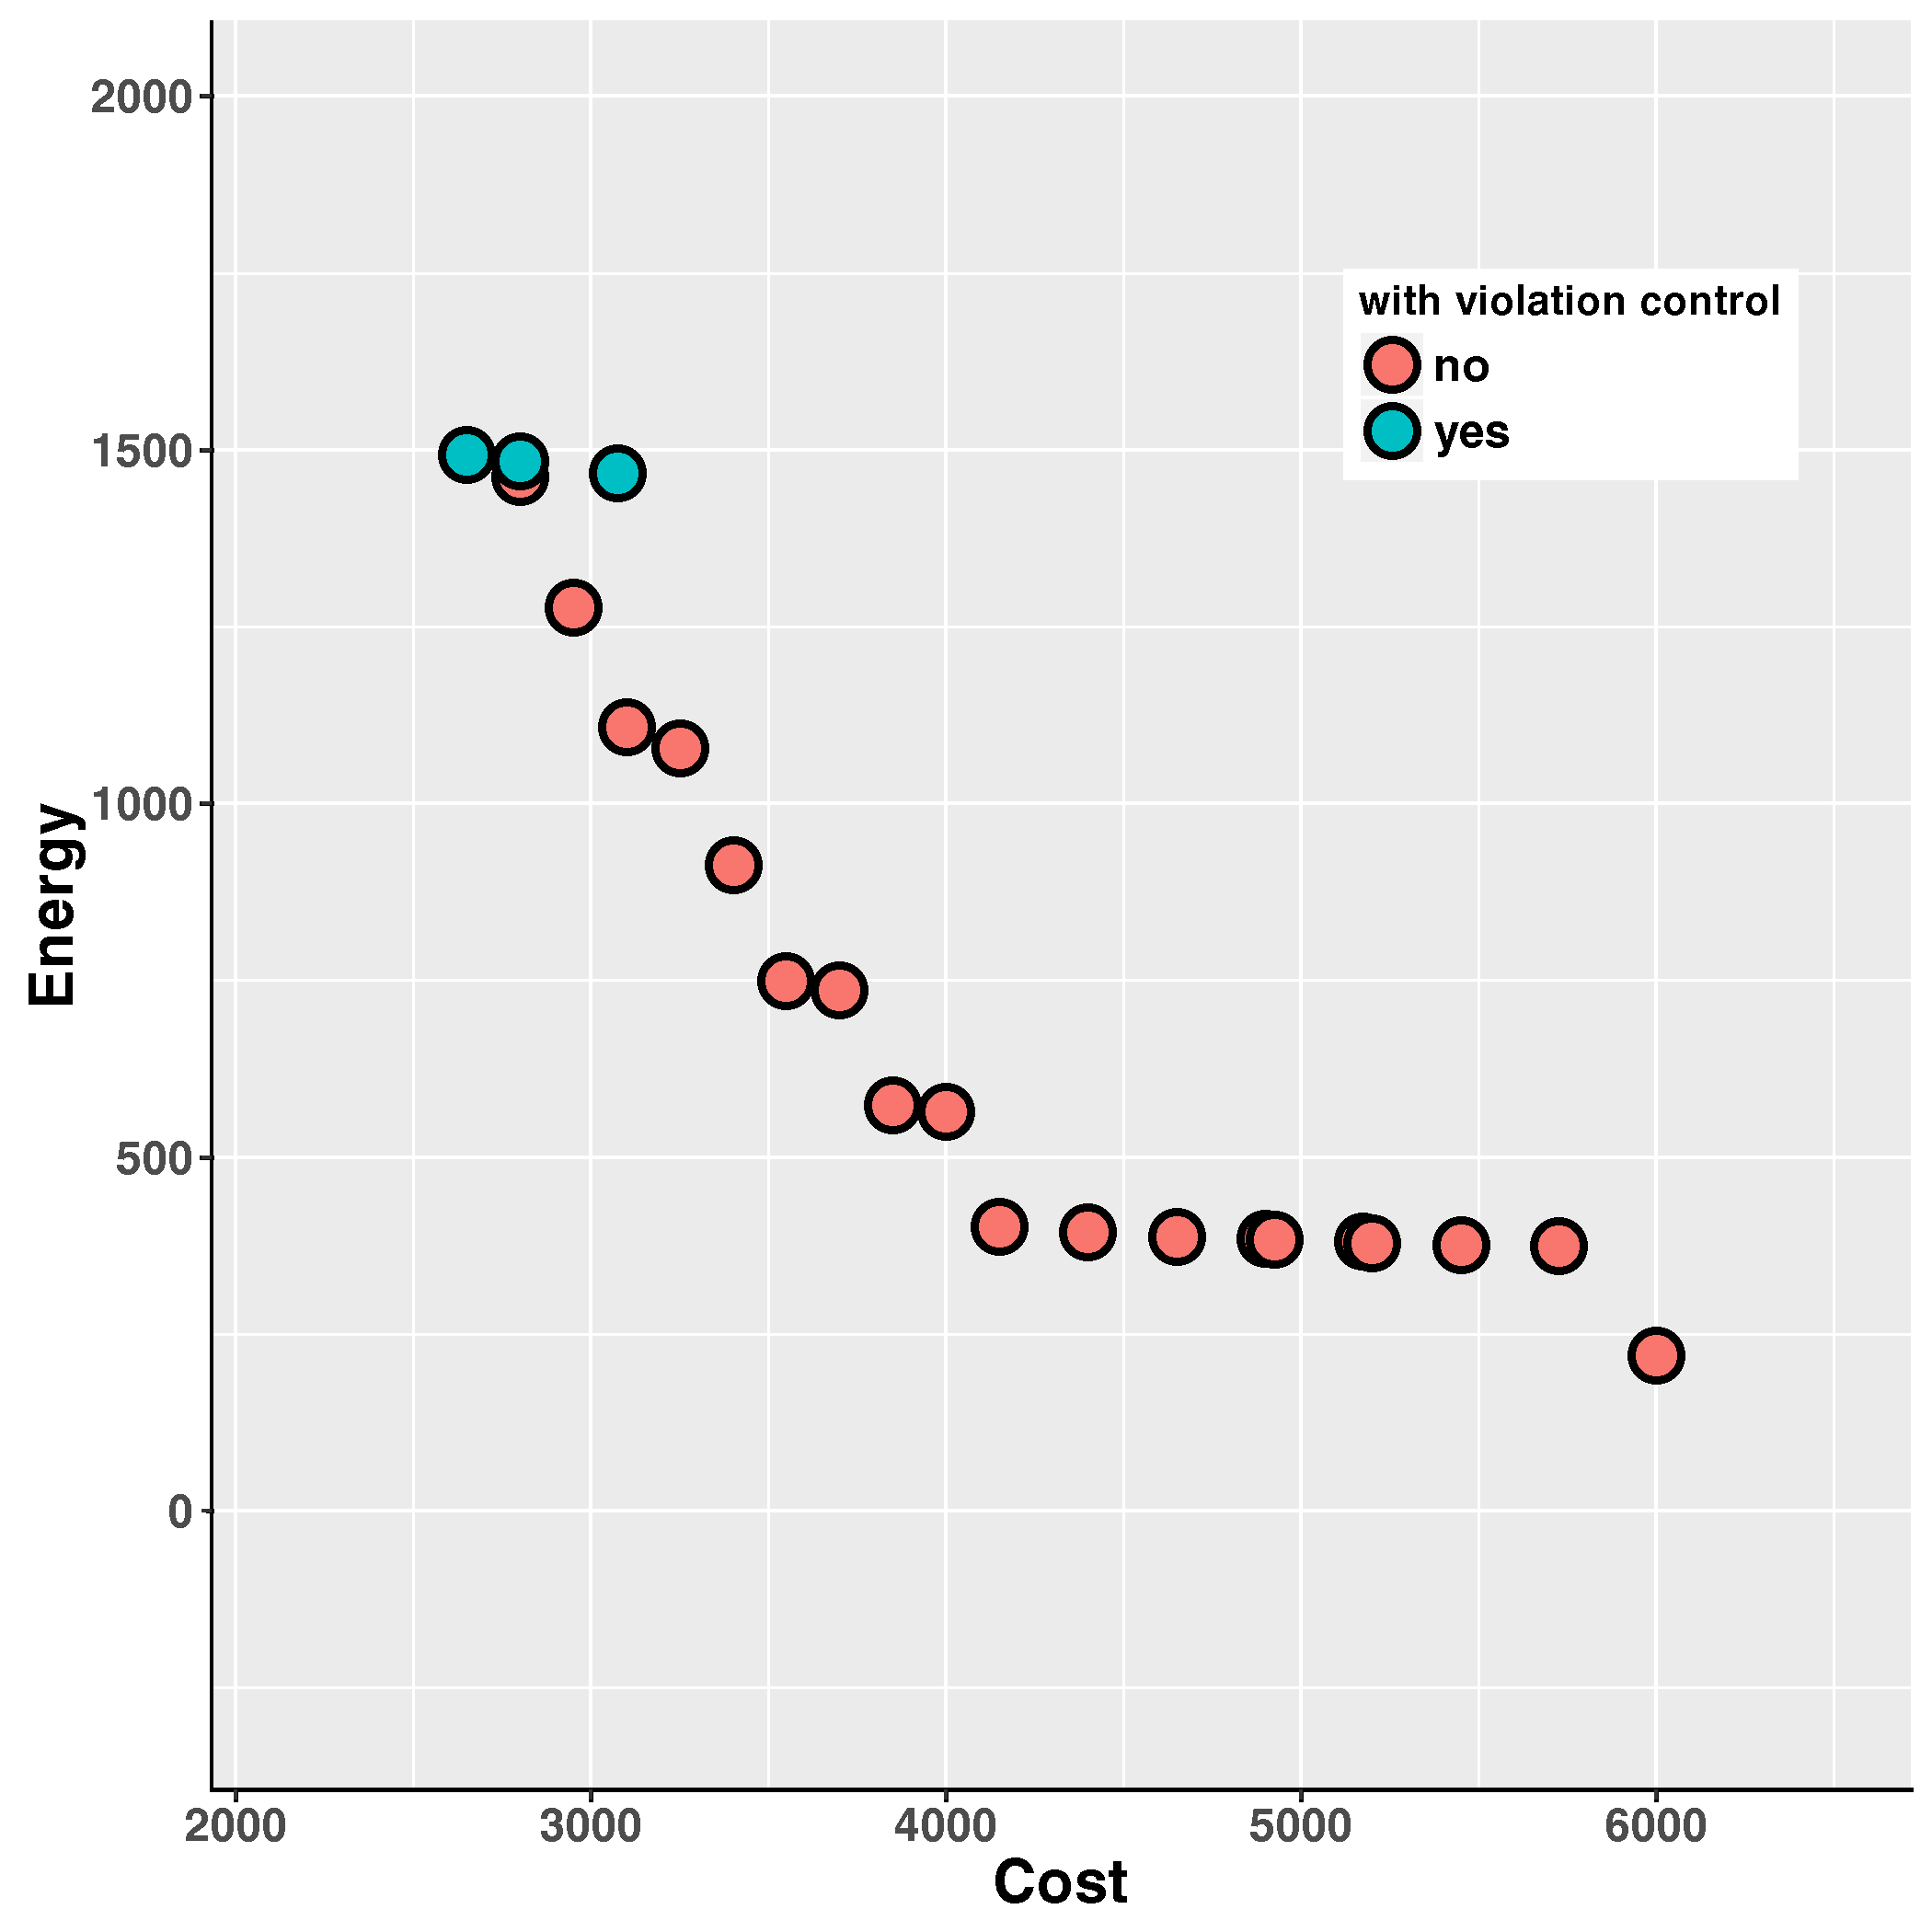
\includegraphics[width=\textwidth]{pics/preliminary/1/evolve.png}
   \caption{Problem 1}
   \label{fig:a}
   \end{subfigure}
   \begin{subfigure}[b]{0.45\textwidth}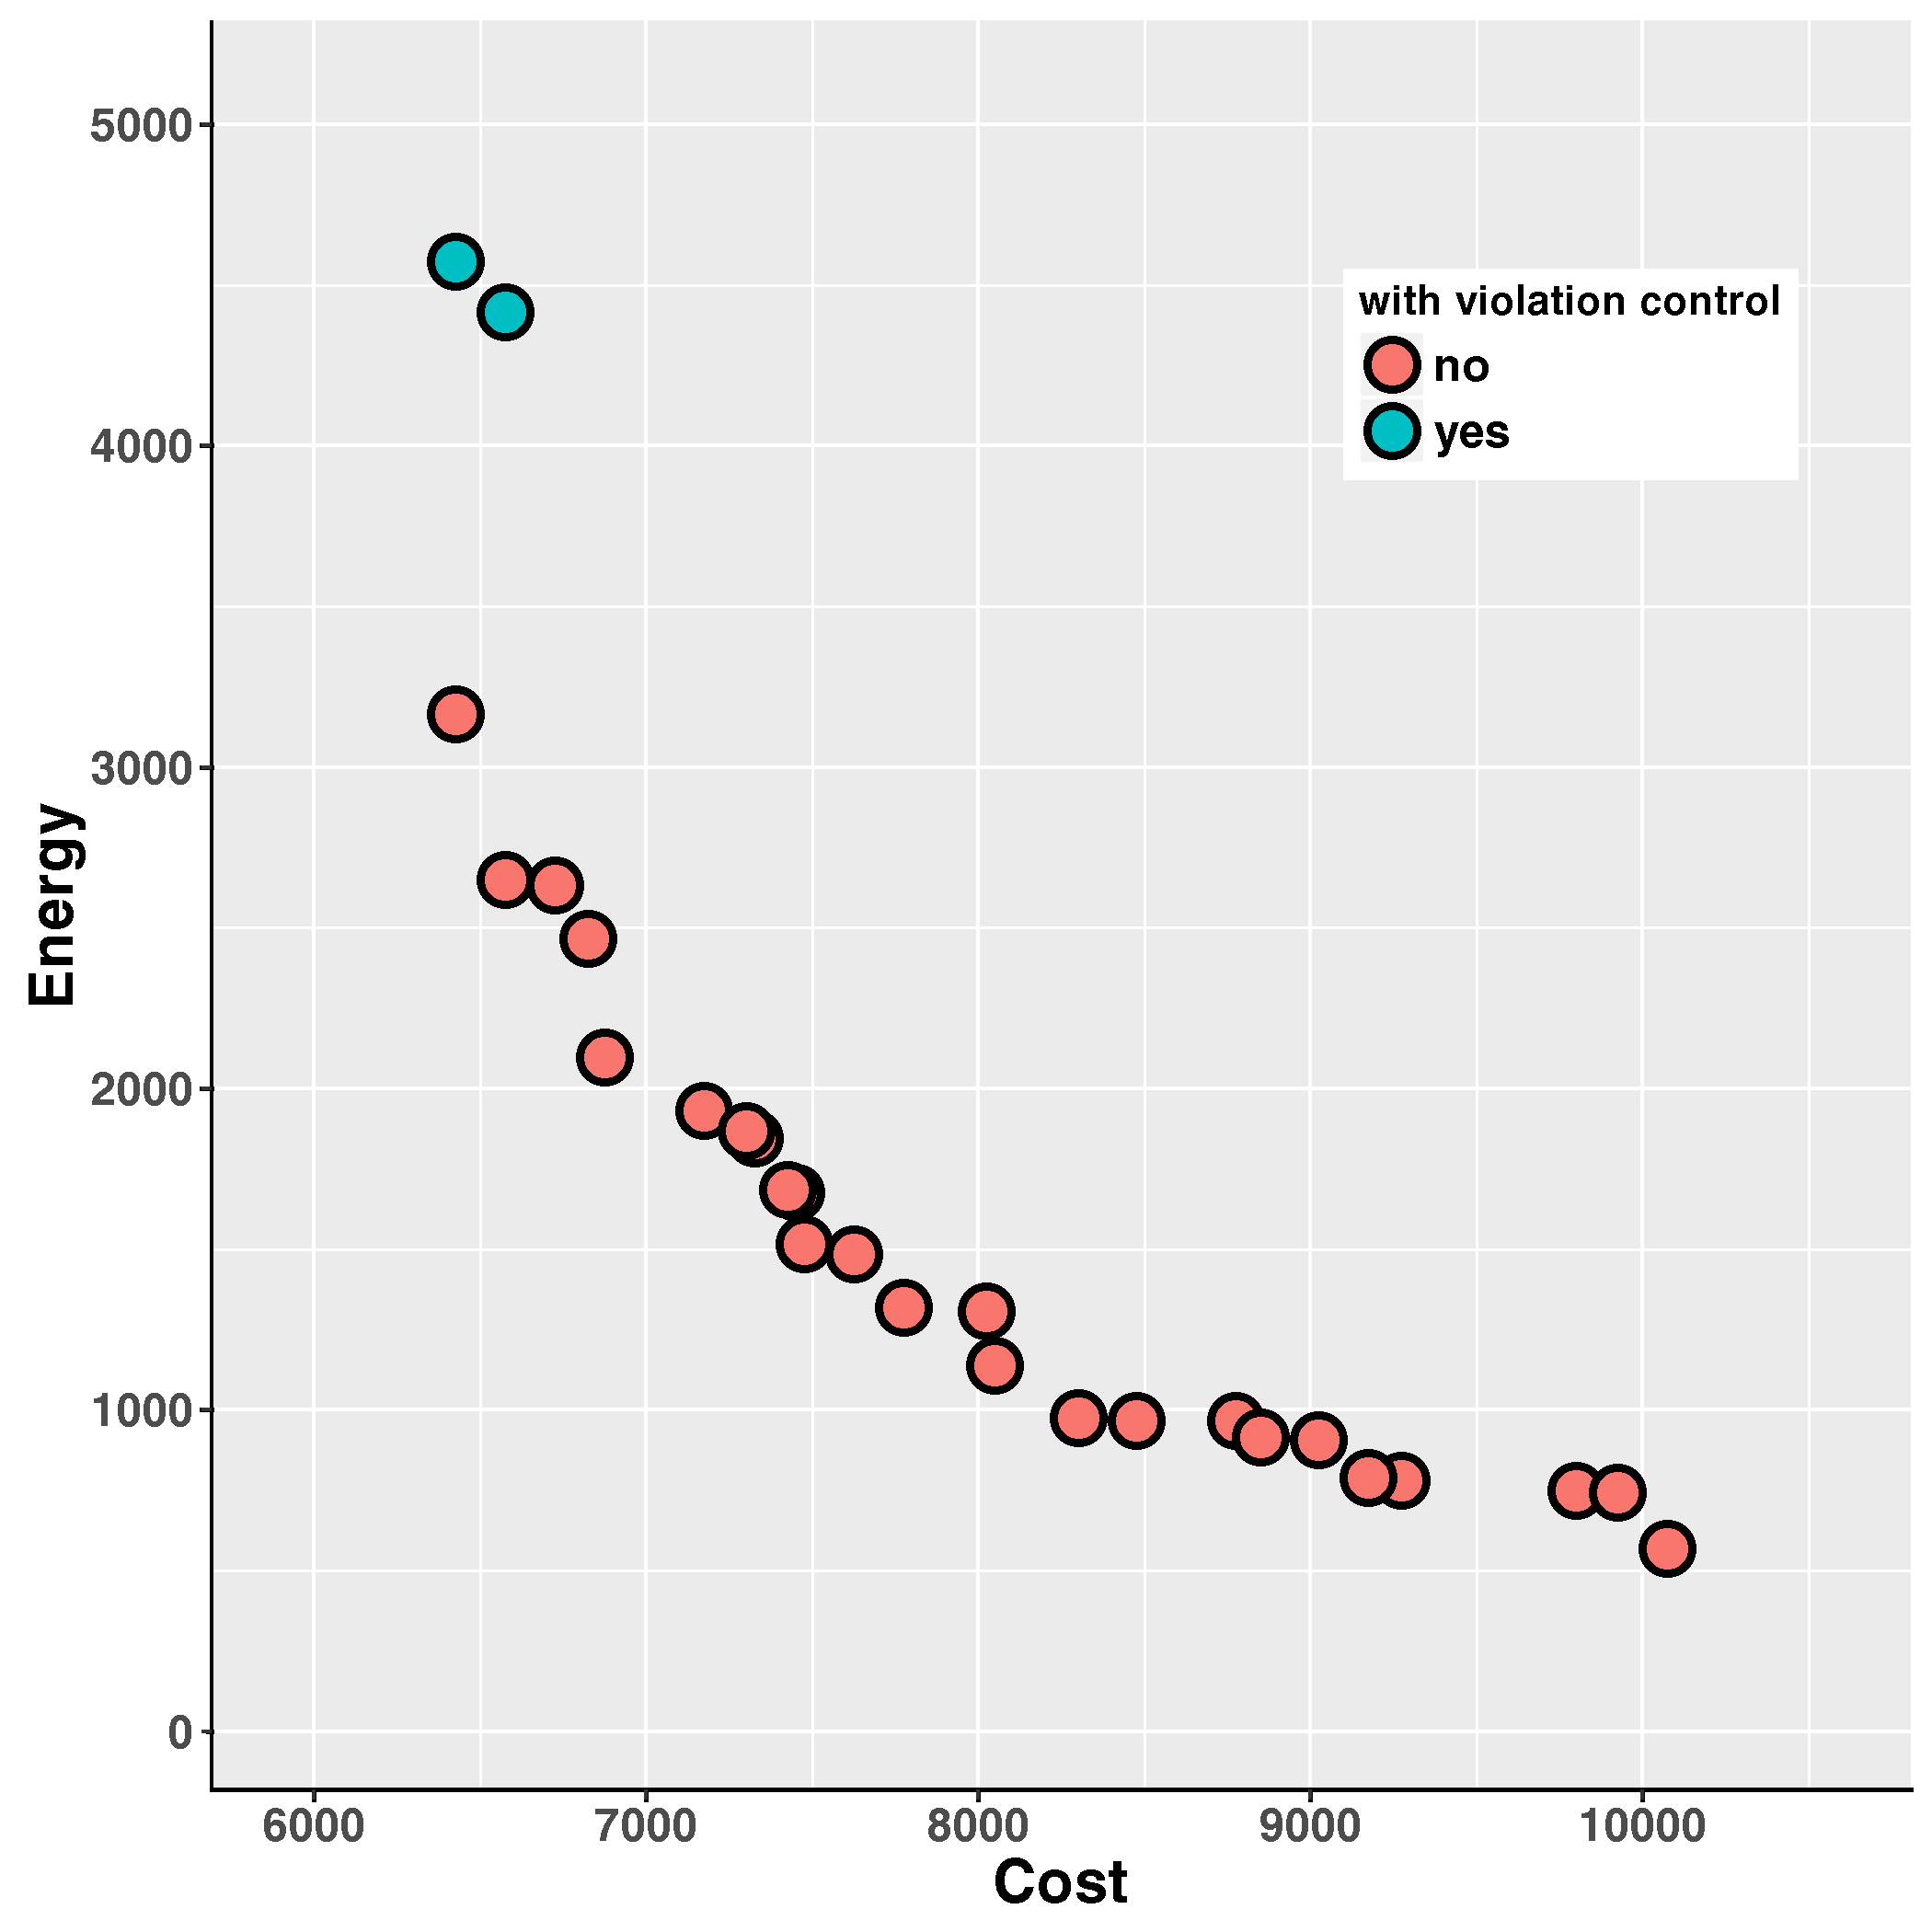
\includegraphics[width=\textwidth]{pics/preliminary/2/evolve.png}
   \caption{Problem 2}
   \label{fig:b}
   \end{subfigure}
   \begin{subfigure}[b]{0.45\textwidth}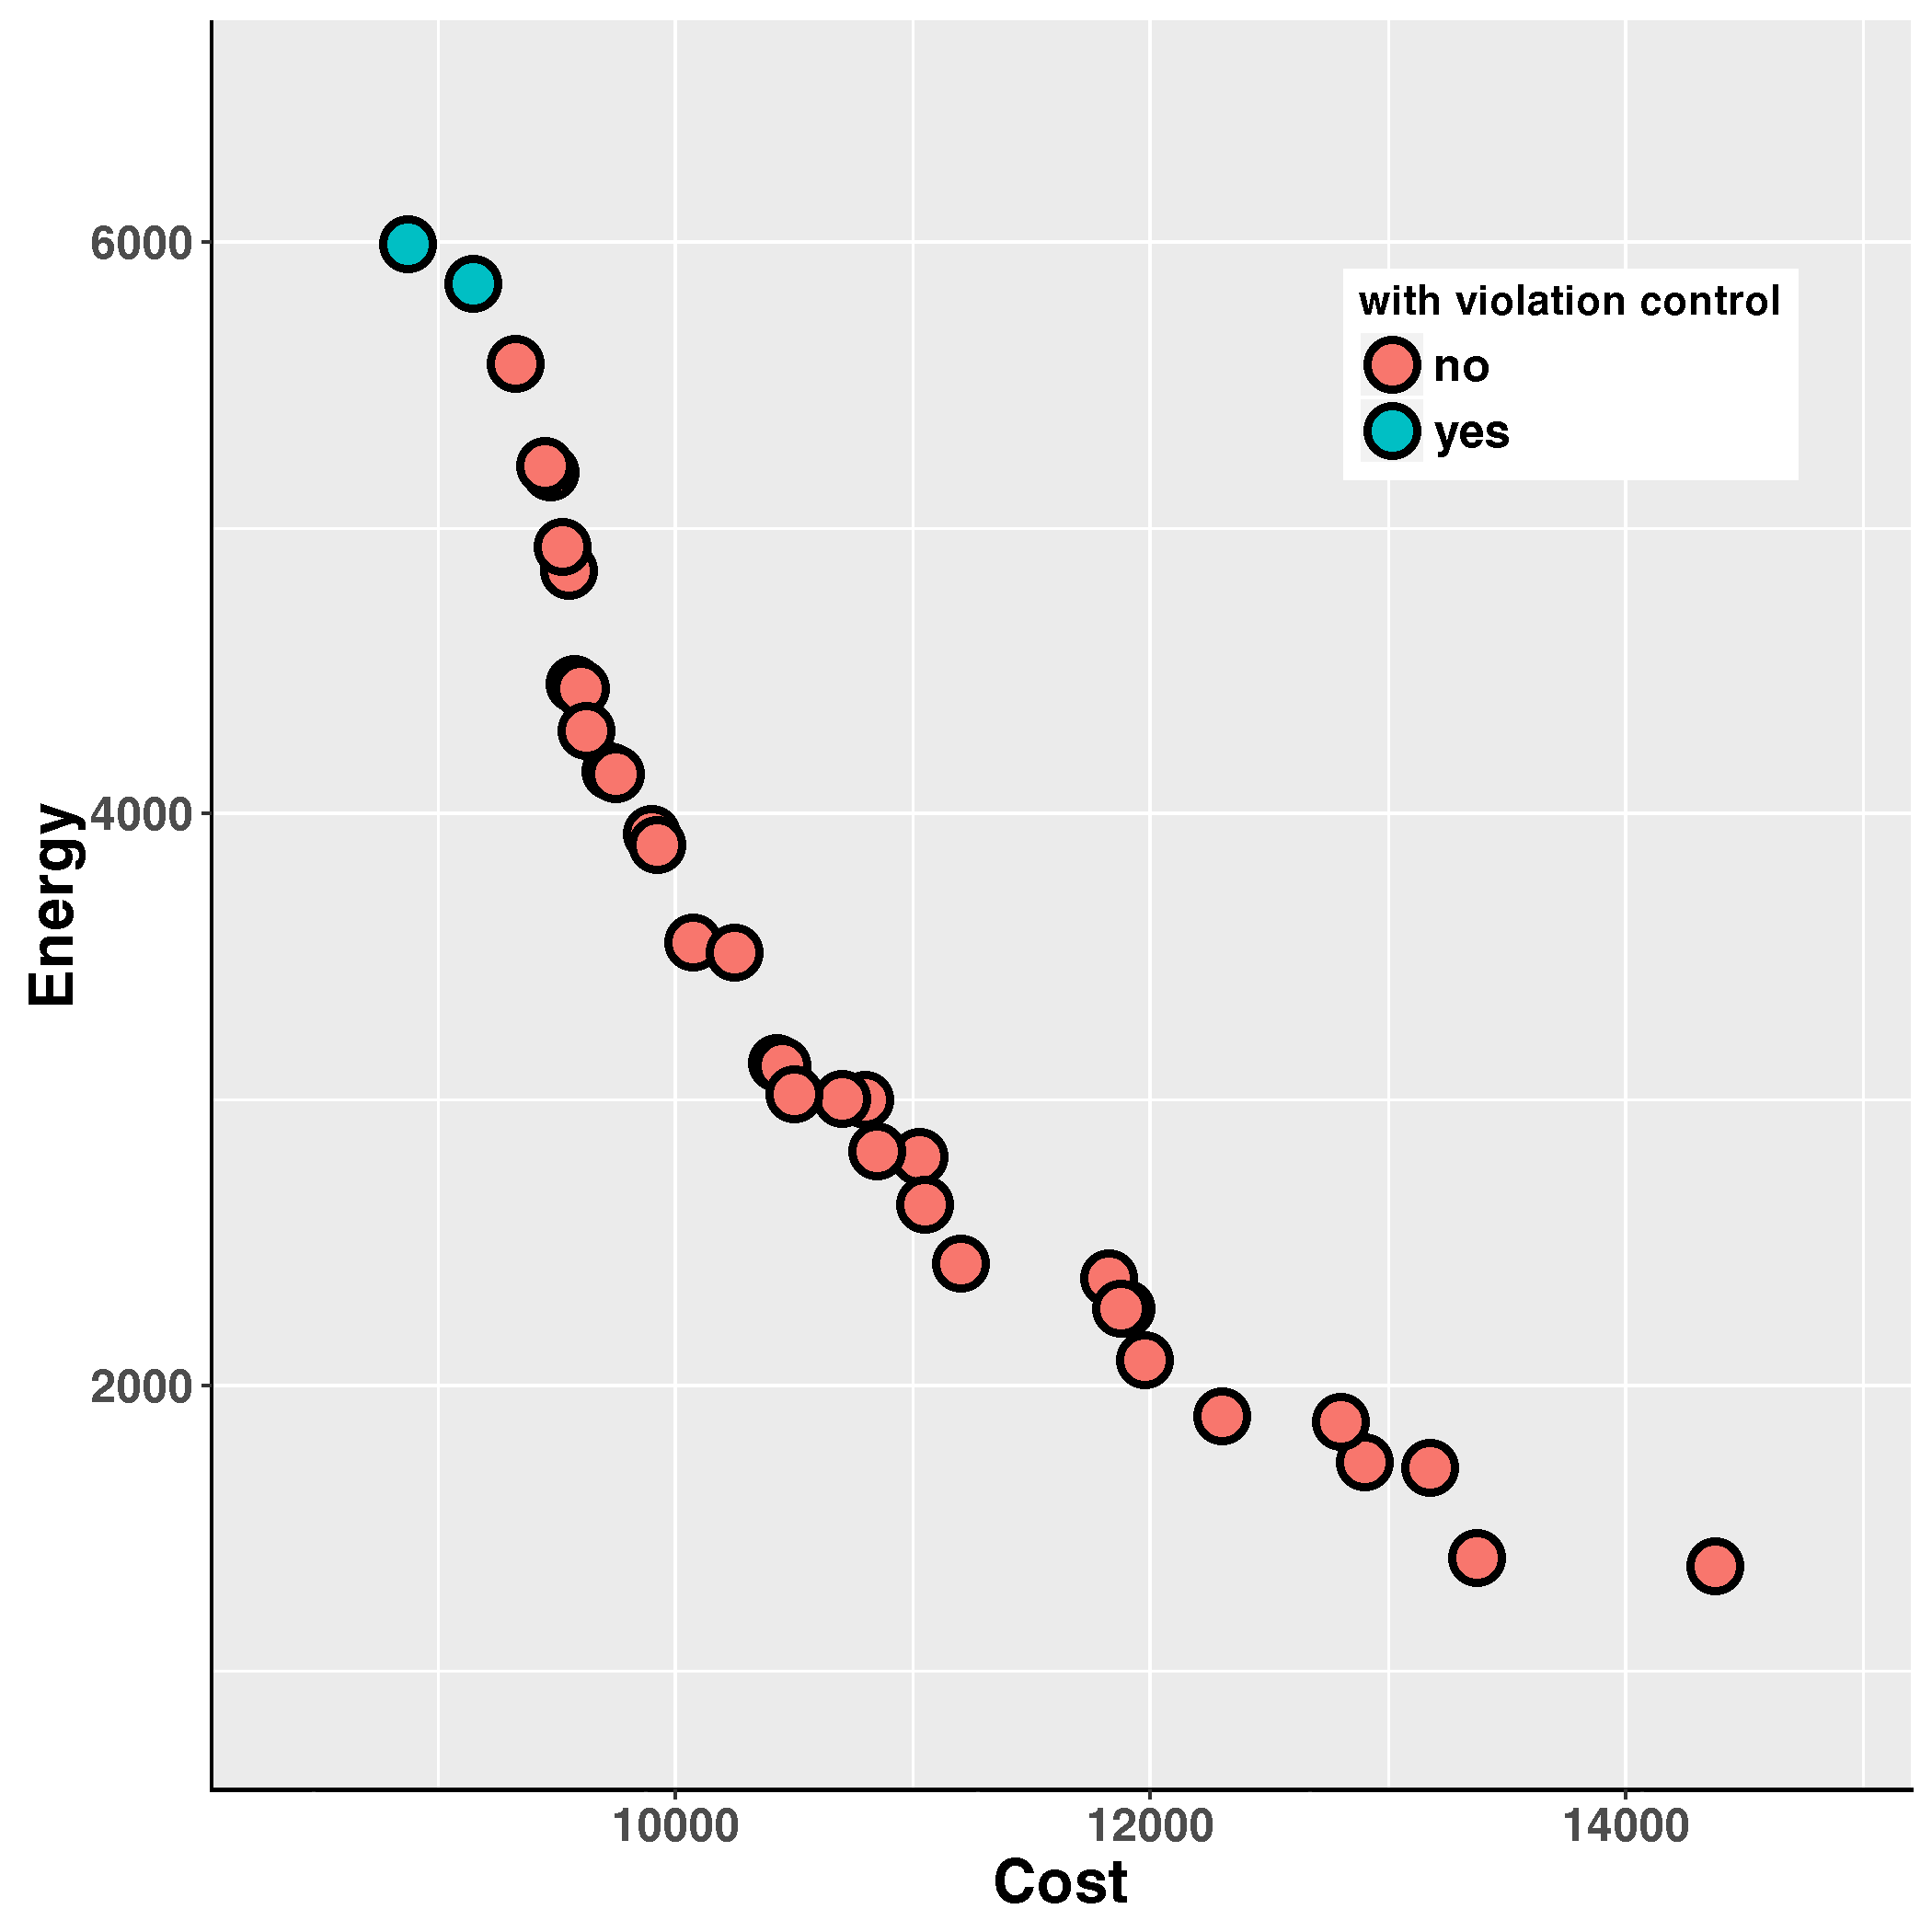
\includegraphics[width=\textwidth]{pics/preliminary/3/evolve.png}
   \caption{Problem 3}
   \label{fig:c}
   \end{subfigure}
   \begin{subfigure}[b]{0.45\textwidth}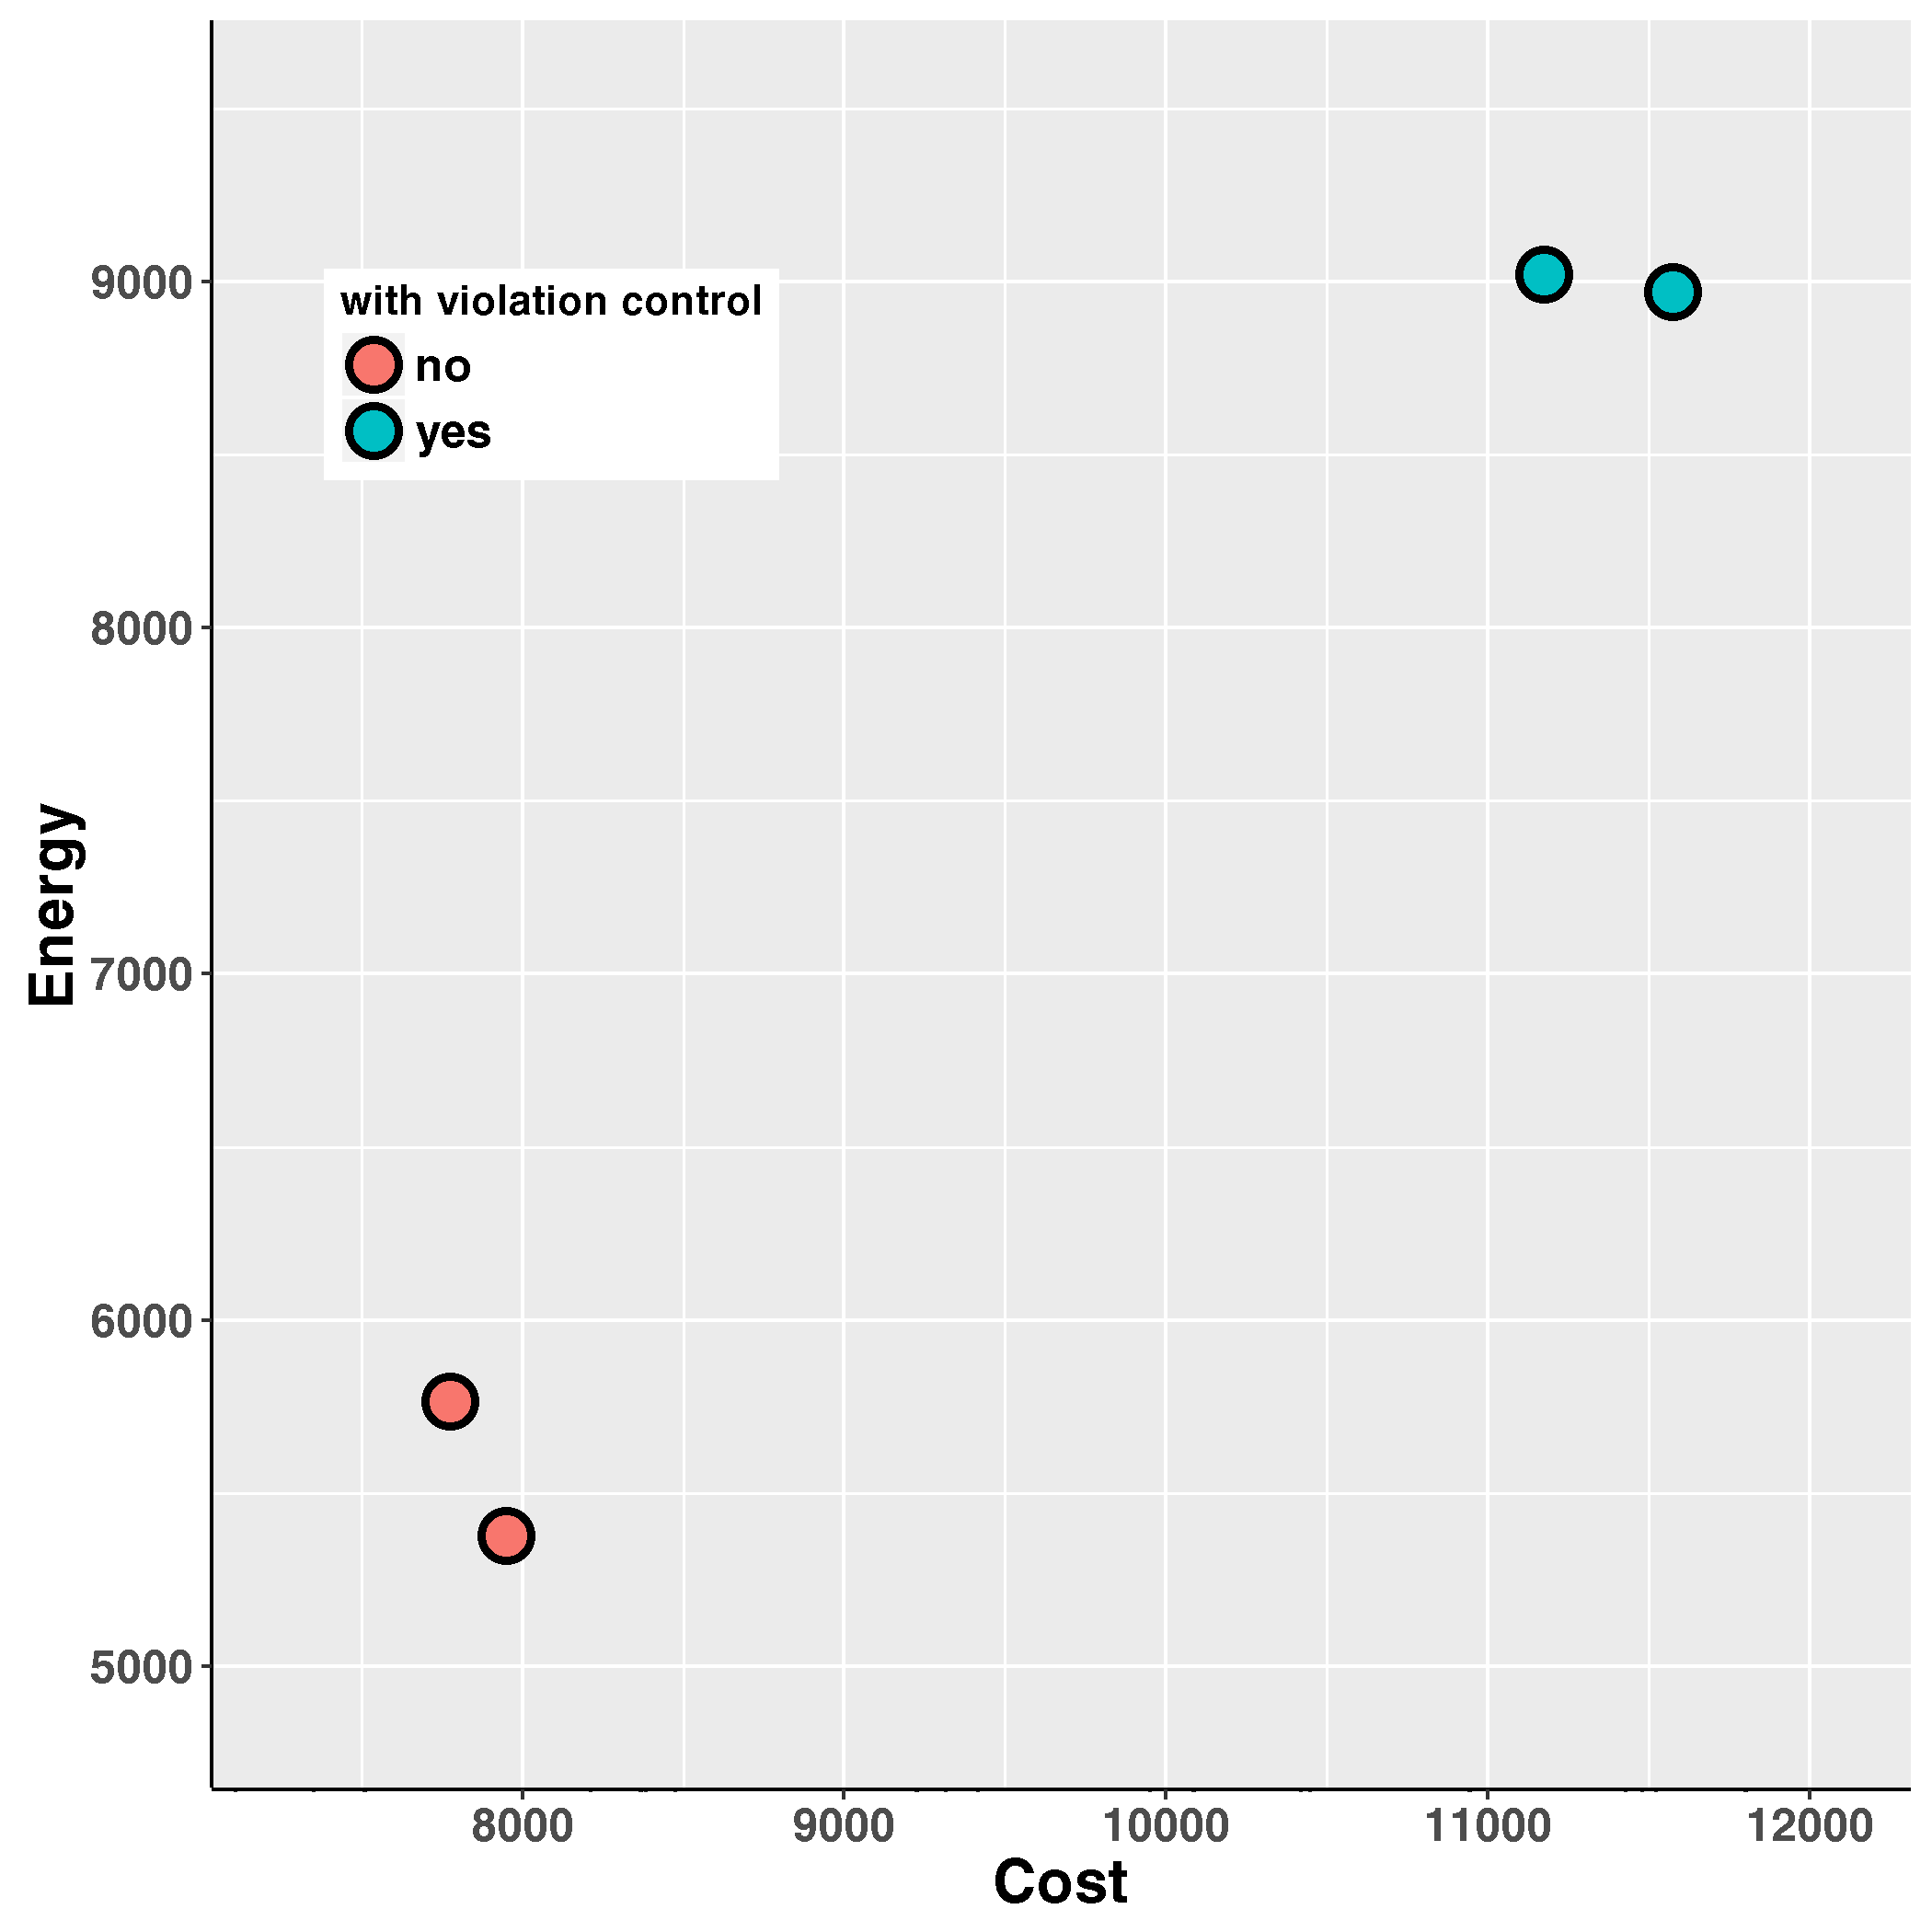
\includegraphics[width=\textwidth]{pics/preliminary/4/evolve.png}
   \caption{Problem 4}
   \label{fig:d}
   \end{subfigure}
   \begin{subfigure}[b]{0.45\textwidth}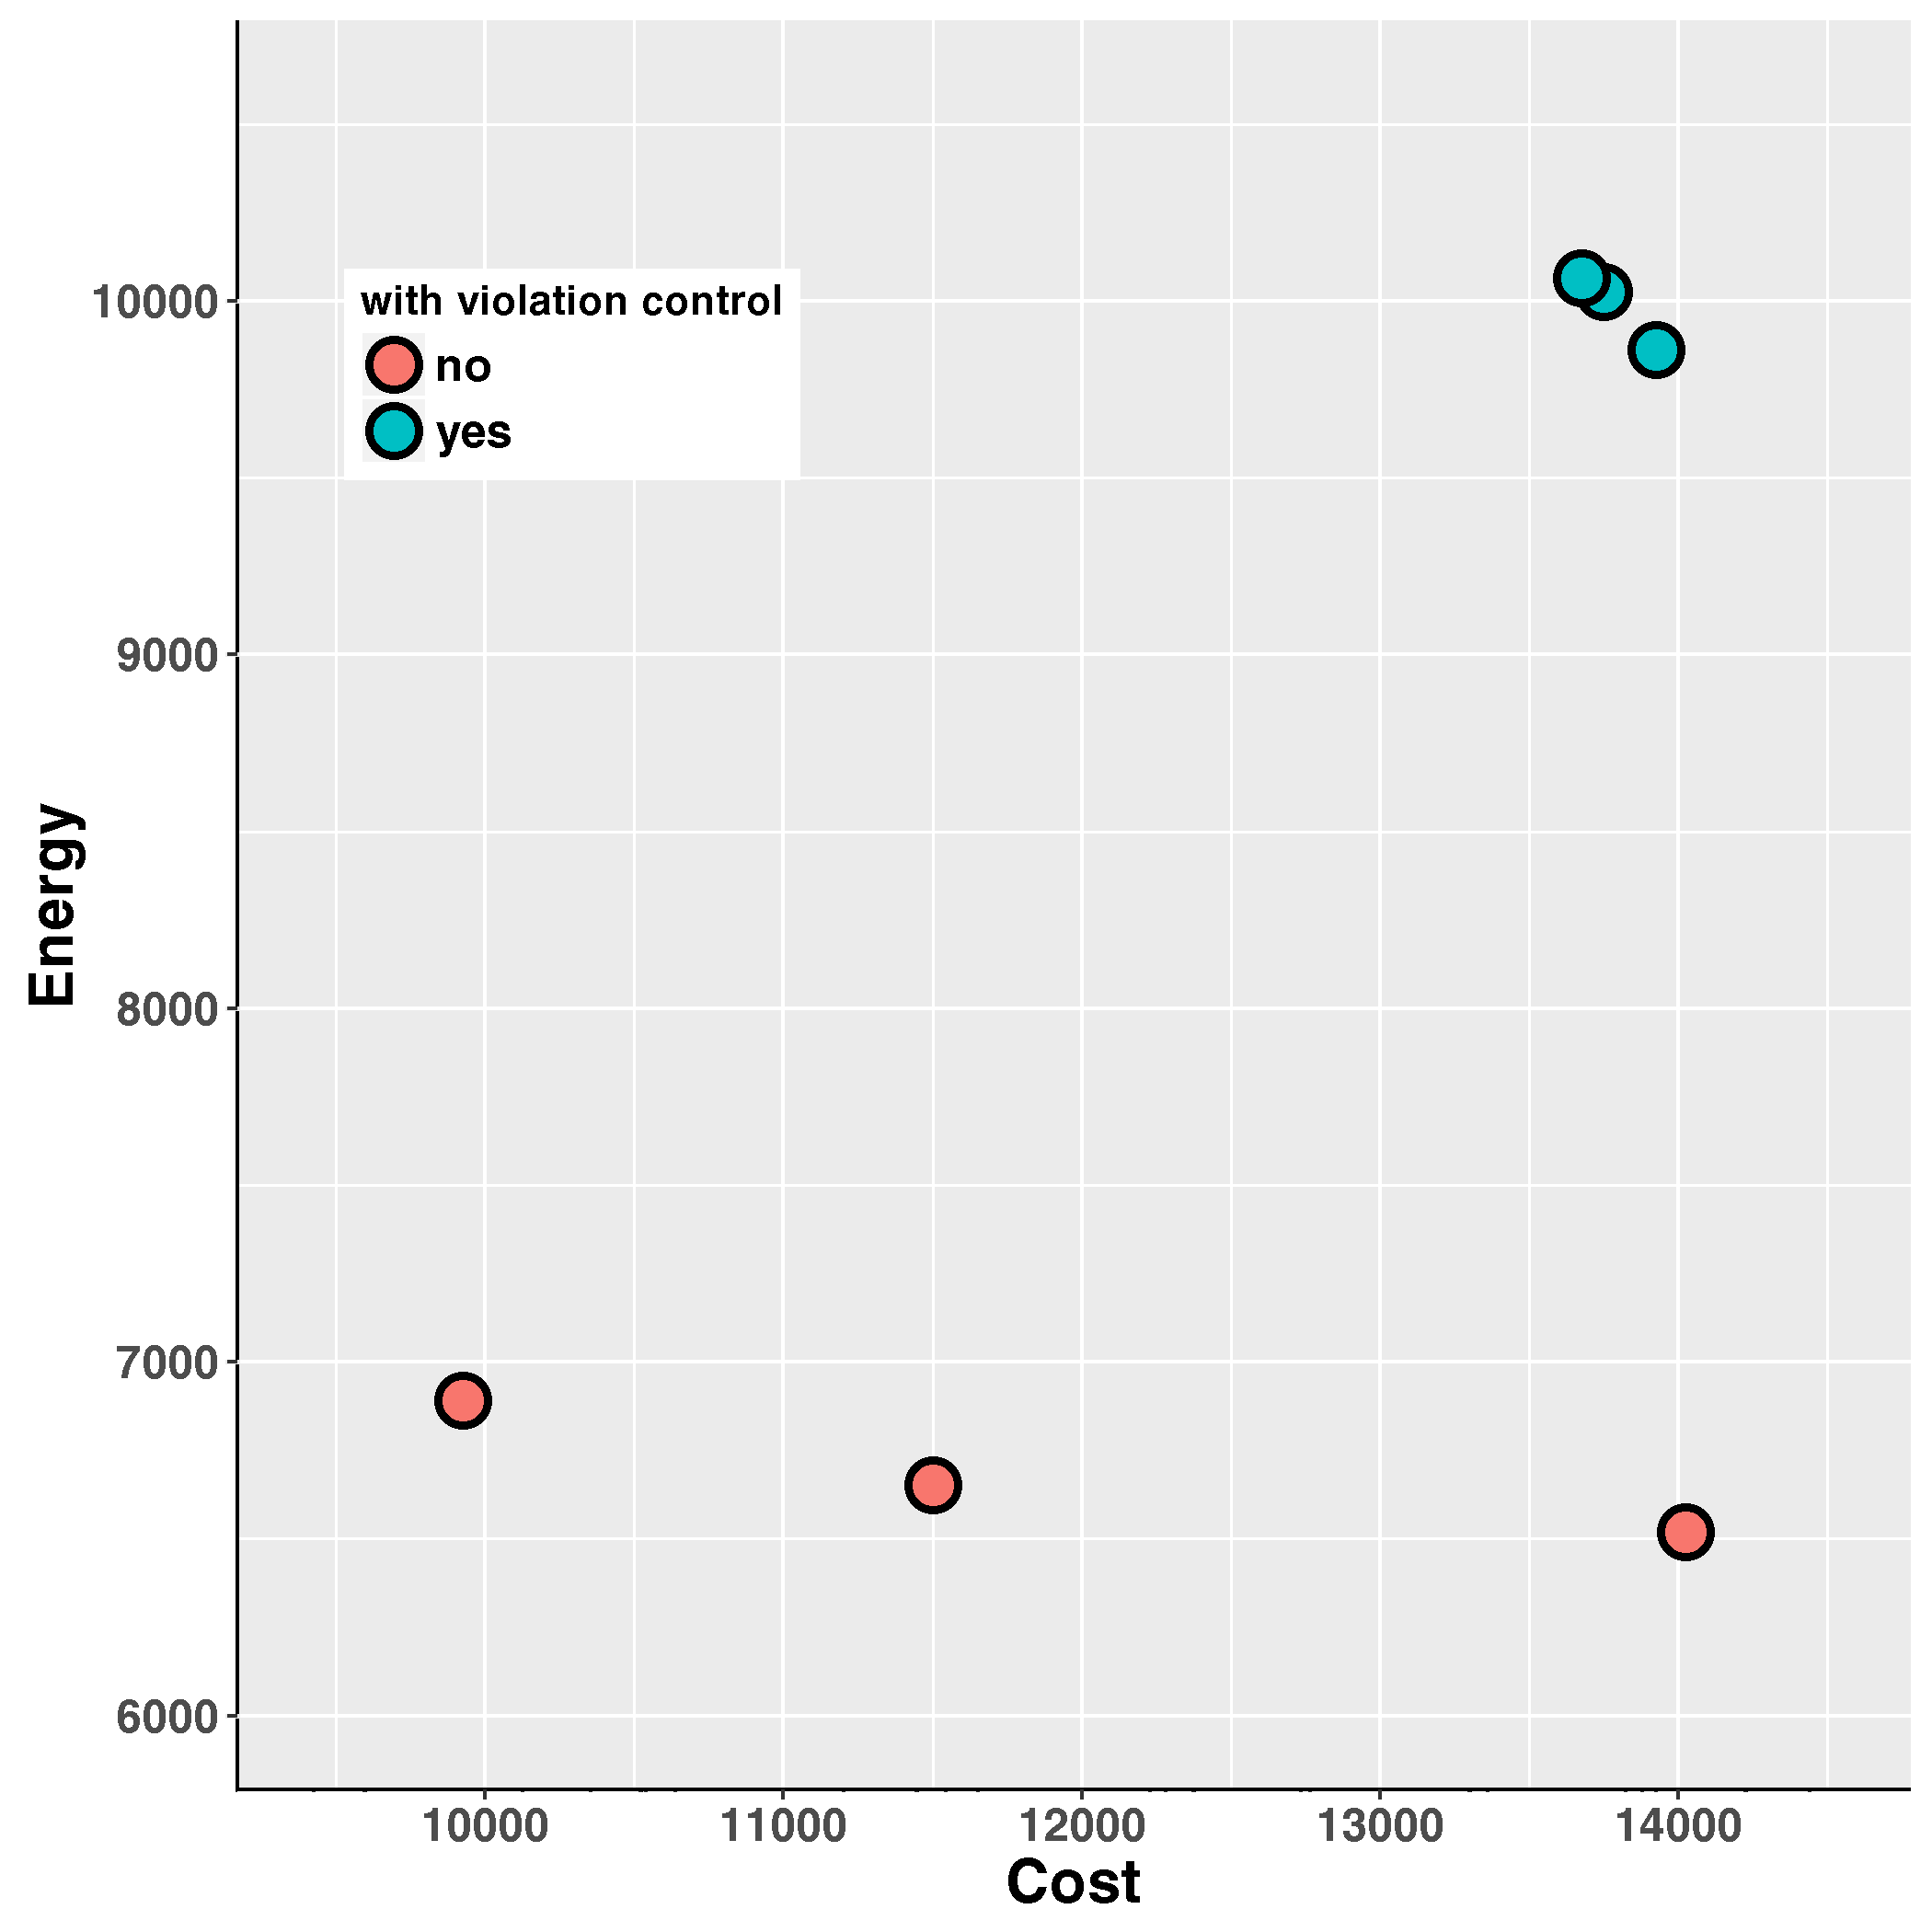
\includegraphics[width=\textwidth]{pics/preliminary/5/evolve.png}
   \caption{Problem 5}
   \label{fig:e}
   \end{subfigure}
     \begin{subfigure}[b]{0.45\textwidth}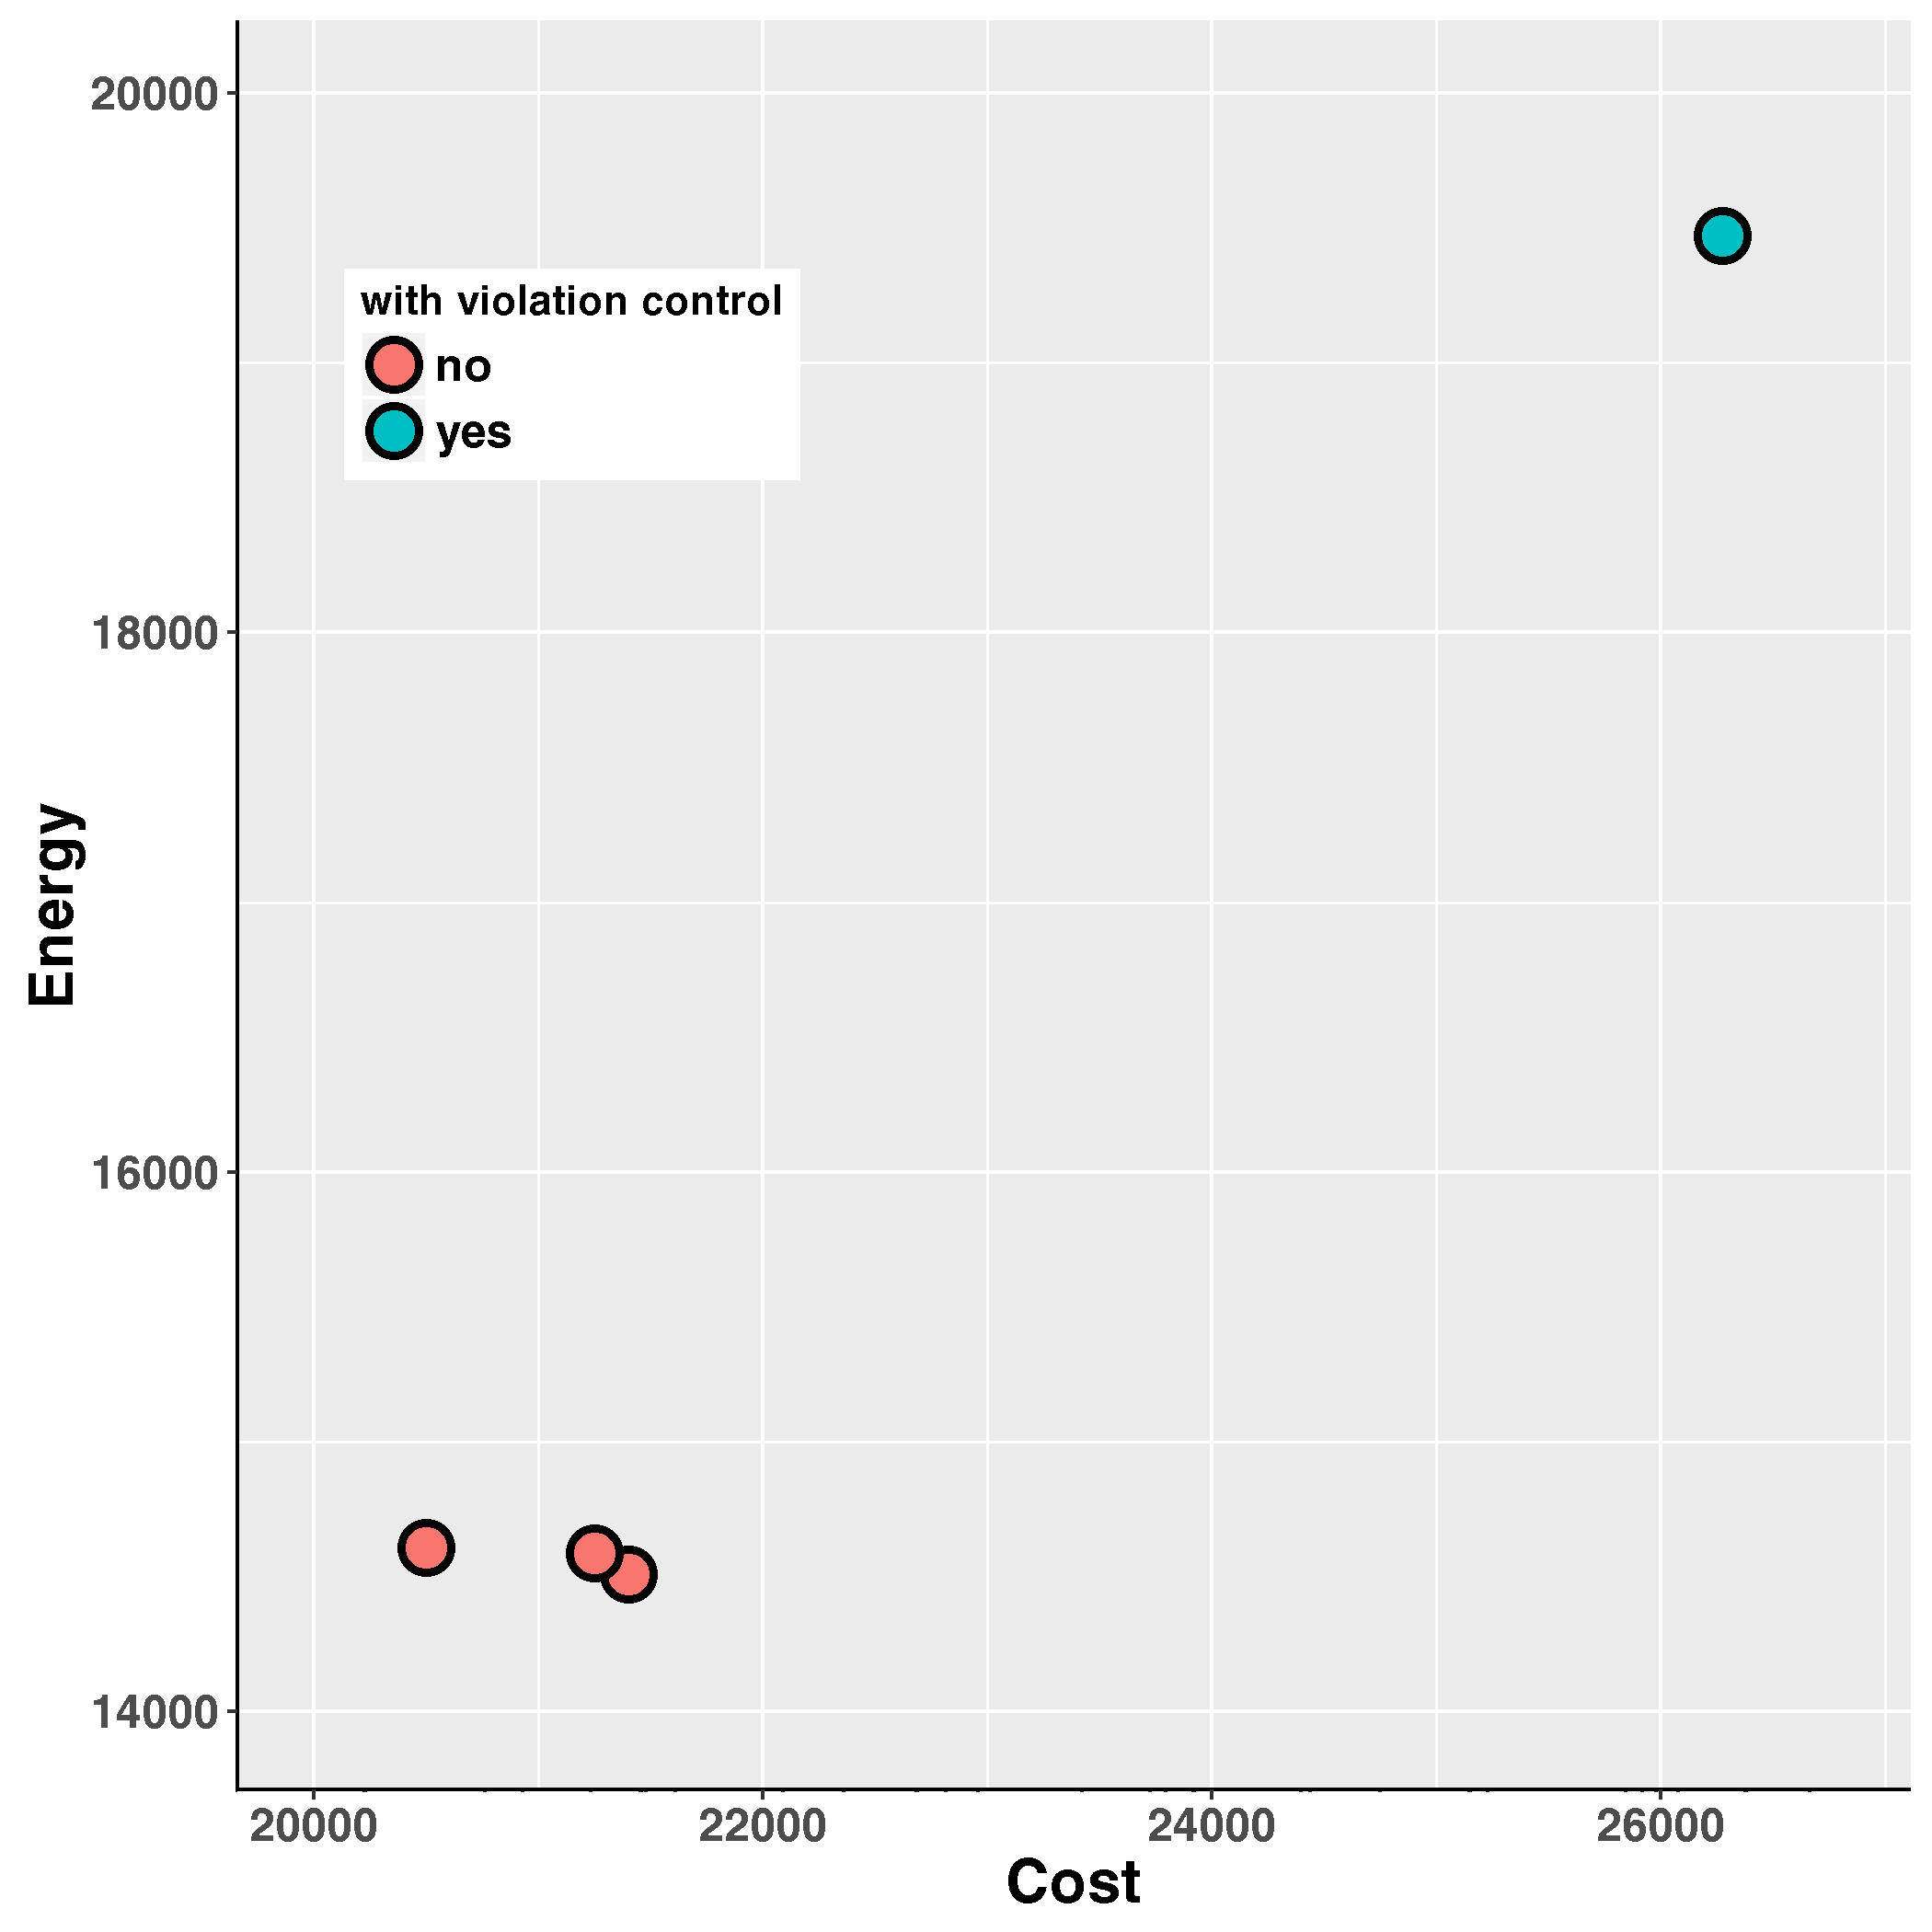
\includegraphics[width=\textwidth]{pics/preliminary/6/evolve.png}
   \caption{Problem 6}
   \label{fig:f}
   \end{subfigure}
   \caption{non-dominated solutions comparison between selection with violation control and without violation control}
   \label{fig:dynamicFunctions}
\end{figure}


\begin{table*}[!ht]
\centering
\caption{Comparison between two Mutation methods}
\label{tab:mutations}
\begin{tabular}{@{}cllll@{}}
\toprule
Problem & \multicolumn{2}{c}{roulette wheel mutation} & \multicolumn{2}{c}{Greedy mutation}   \\ \midrule
        & cost fitness         & energy fitness       & cost fitness      & energy fitness    \\
1       & 2664.6 $\pm$ 66.4      & 1652.42 $\pm$ 18.2     & 2661.7 $\pm$ 56.9   & 1653.2 $\pm$ 18.2   \\
2       & 6501.1 $\pm$ 130.2     & 4614.0 $\pm$ 110.7     & 6495.37 $\pm$ 110.7 & 4132.5 $\pm$ 80.4   \\
3       & 8939.2 $\pm$ 118.5     & 6140.7 $\pm$ 204.0     & 9020.5 $\pm$ 204.0  & 5739.6 $\pm$ 148.6  \\
4       & 11633.7 $\pm$ 301.1    & 9301.9 $\pm$ 254.0     & 12900.6 $\pm$ 243.0 & 9376.3 $\pm$ 120.9  \\
5       & 14102.0 $\pm$ 231.7    & 10164.8 $\pm$ 238.9    & 14789.2 $\pm$ 238.8 & 9876.3 $\pm$ 120.9  \\
6       & 27194.3 $\pm$ 243.0    & 19914.4 $\pm$ 307.5    & 27654.2 $\pm$ 307.5 & 19187.1 $\pm$ 176.6 \\ \bottomrule
\end{tabular}
\end{table*}

As we conducted the experiment for 30 runs, we first obtain an average non-dominated set over 30 runs by collecting the results from a specific generation from all 30 runs, and then apply a non-dominated sorting over them.

Firstly, we show the non-dominated solutions evolve along with the evolution process in Figure \ref{fig:evolve}.
These results come from selection method without violation control. 
As it illustrated, different colors represent different generations from 0th to 200th. 
For problem 1, because the problem size is small, the algorithm converged before 100 generations. Therefore, the non-dominated set from the 100th and 150th generations are overlapping with results from the 200th generation. For problem 2 and problem 3, it clearly shows the improvement of fitness values. For problem 4 onwards, the algorithm can only obtain a few solutions as the problem size is large, it is difficult to find solutions.

Then, the non-dominated sets of the last generation from two selection methods are compared in Figure \ref{fig:dynamicFunctions}. There are much fewer results are obtained from the violation control method throughout all cases. For the first three problems, the non-dominated set from the violation control method has similar quality
as the no violation control method. From problem 4 onwards, the results from selection with violation control are much worse in terms of fitness values. However, most of the results from non-violation control selection have a high violation rate. That is, the method without violation control is stuck in the infeasible regions and provide high-violation rate solutions. 

From figure \ref{fig:violations}, we can observe the violation rate between two methods.
It proves violation control has a great ability to prevent the individual from searching the infeasible region. On the other hand, without violation control, although, the algorithm can provide more solutions with better fitness values, most of them have a high violation rate over 10\% which are not very useful in reality.

As we mentioned in previous section, the mutation rate and consolidation factor are set differently for the two methods. For the method with violation control, the mutation rate is set to 0.9 and the consolidation factor $c$ is set to 0.01, this is because the feasible region is narrow and scattered. In order to avoid stucking in the local optima, a large mutation rate can help escape local optima. For the factor $c$, a larger percentage would easily lead the algorithm to infeasible regions. Therefore, it is set to a small number.





\begin{figure}
\centering
  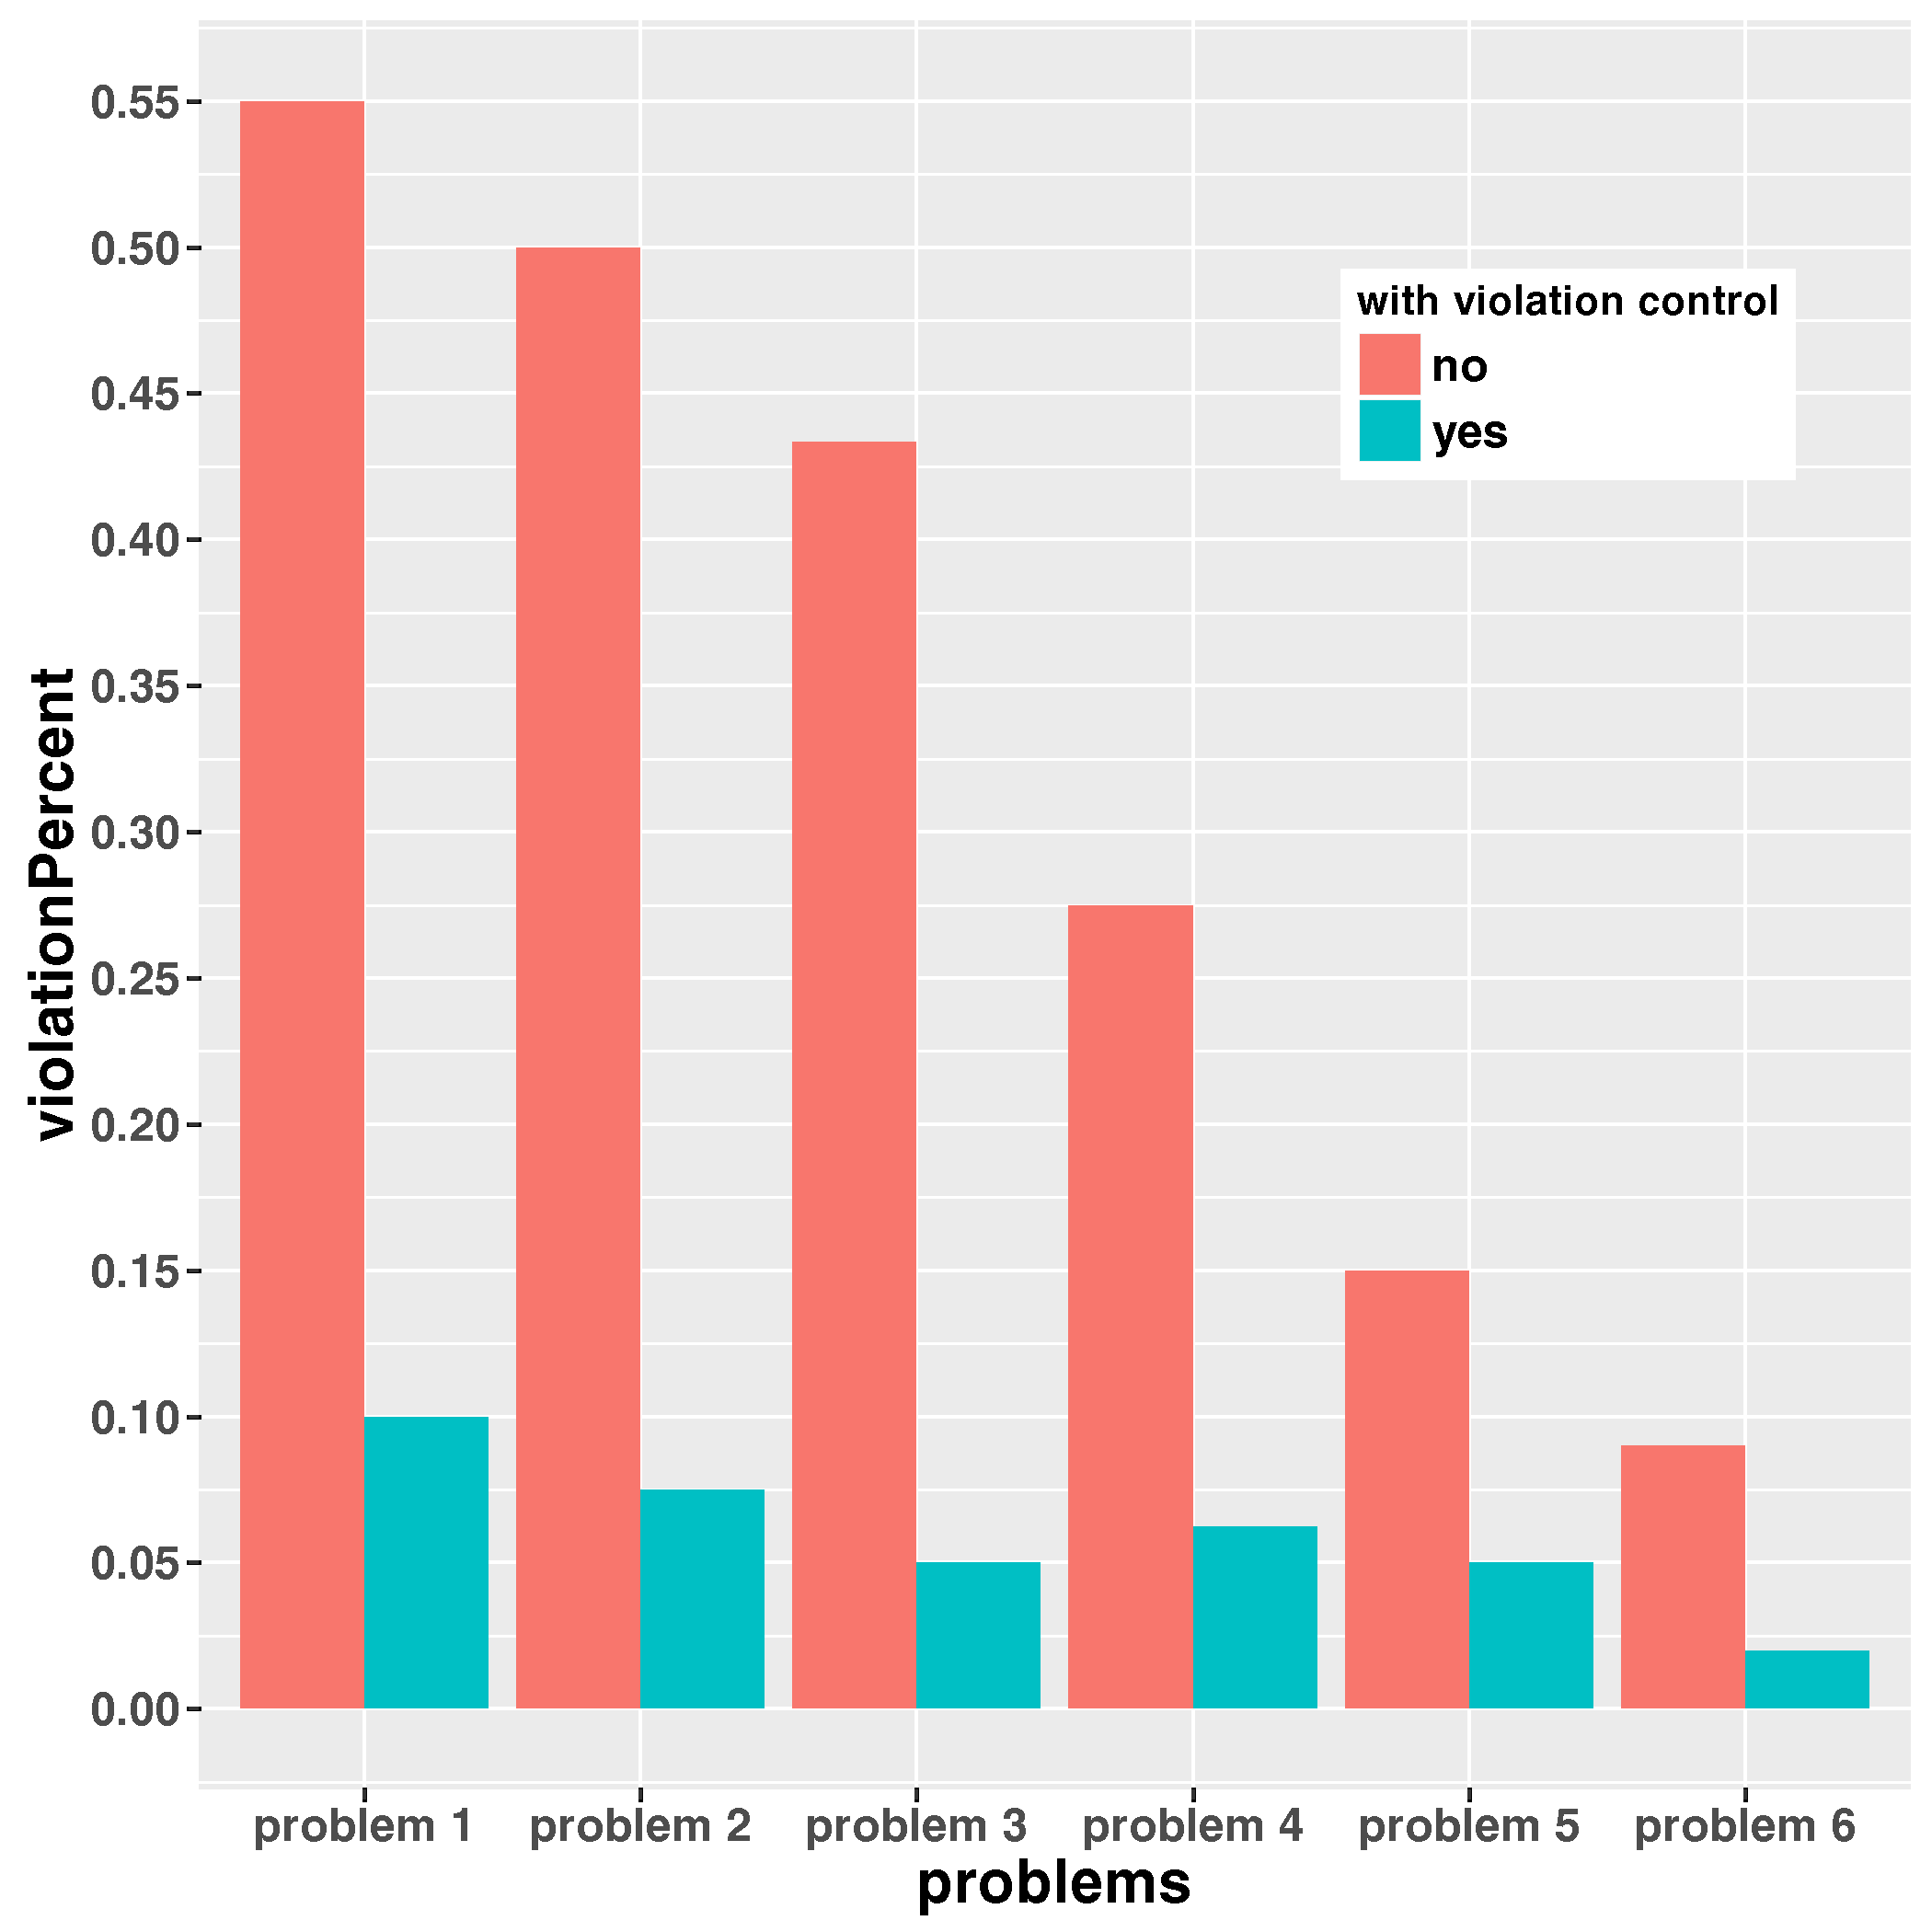
\includegraphics[width=.7\textwidth]{pics/preliminary/violations.png}
  \caption{Violation Percentage comparison between selection with violation control and without violation control}
  \label{fig:violations}
\end{figure}



\begin{flushleft}\textbf{Mutation with roulette wheel vs. Mutation with greedy algorithm}\end{flushleft}
Table \ref{tab:mutations} shows the fitness value comparison between mutation methods. According
to statistics significant test, there is little difference between methods. The possible reason
is the consolidation factor is set to 0.01. In each mutation iteration, there is only 1\% probability
that a service will be consolidated in an existed VM, therefore, the influence between
different consolidation strategies is trivial.





\section{Conclusion}
\label{sec:con}

In this paper, we first propose a multi-objective formulation of a two levels of bin packing problem, web service resource allocation in Cloud. It solves the resource allocation in IaaS and SaaS at the same time. Two objectives, minimizing the cost from service providers' perspective and minimizing the energy consumption from cloud provider's objective are achieved. Secondly, we propose a NSGA-II based algorithm with specific designed genetic operators to solve the problem. The results are
compared with different variances of the algorithm. The results show our approach can solve the very complicate
optimization problem.

With current work as a baseline, in future work, we could improve the quality of solutions as well as provide better violation control mechanisms.

% In recent years, virtualization technology has evolved to allow finer granularity resource management.
% A recent development of Container technique \cite{Soltesz:2007cu} has driven the attention of both industrial and academia.
% Container is an operating system level of virtualization which means multiple containers can be installed in a same operating system (see Figure \ref{fig:comparison} right-hand side). Each container provides an isolated environment for an application. In short, a VM is partitioned into smaller manageable units.}
\chapter{Proposed Contributions and Project Plan}\label{C:con}

This thesis will contribute to the field of Cloud Computing by proposing novel solutions for the joint allocation of container and VM, and to the field of Evolutionary Computation by proposing new representations and genetic operators in evolutionary algorithms. The proposed contributions of this project are listed below:

\begin{enumerate}
	\item Propose a new model for the joint allocation of container and VM problem.
	New representations will be proposed to problem.
	The first EC-approach to solve the problem. 
	Reduce the energy consumption of data centers.
	\item Propose a new robustness measure for time-dependent server consolidation problem. New optimization algorithms not only consider the two-level of packing problem but also take the previous and next consolidation into considered.
	\item Develp a GP-based hyper-heuristic approach to automatically generate dispatching rules for dynamic server consolidation problem. New functional and primitive set for constructing useful dispatching rules will be studied. New genetic operations and representations will be proposed.
	\item Develop a preprocessing algorithm to reduce the number of variables in a large scale static consolidation problem without scacrificing too much performance. Useful features of server consolidation problem will be studied.
\end{enumerate}

\section{Overview of Project Plan}
Six overall phases have been defined in the initial research plan for this PhD project, as
shown in Figure \ref{fig:}. The first phase, which comprises reviewing the relevant literature, investigating both VM-based and container-based server consolidation algorithms, and producing the proposal, has
been completed. The second phase, which corresponds to the first objective of the thesis, is
currently in progress and is expected to be finished on time, thus allowing the remaining
phases to also be carried out as planned.

\section{Project Timeline}
The phases included in the plan above are estimated to be completed following the timeline
shown in Figure \ref{}, which will serve as a guide throughout this project. Note that part of the first phase has already been done, therefore the timeline only shows the estimated remaining time for its full completion.

\section{Thesis Outline}
The completed thesis will be organised into the following chapters:
\begin{itemize}
	\item \textit{Chapter 1: Introduction} \\
	This chapter will introduce the thesis, providing a problem statement and motivations, defining research goals and contributions, and outlining the structure of this dissertation.
	\item \textit{Chapter 2: Literature Review} \\
	The literature review will examine in the existing work on VM-based and container-based server consolidation, discussing the fundamental concepts in this field in order to provide the reader with the necessary background. Multiple sections will then follow, 
	considering issues such as static consolidation, dynamic consolidation, and large-scale of consolidation problem. The focus of this review is on investigating server consolidation techniques that are based on Evolutionary Computation.
	\item \textit{Chapter 3: An EC Approach to the joint Allocation of Container and Virtual Machine} \\
	This chapter will establish a new model for the joint allocation of container and virtual machine problem. Furthermore, this chapter will introduce a new bi-level approach to solve this problem. One of the critical aspects of this approach is the representation of solution. Therefore, multiple representations will be proposed, analysed and compared.
	\item \textit{Chapter 4: An EC Approach to the Time-dependent Global Server Consolidation} \\
	In this chapter, a robustness measure of time-dependent server consolidation will be proposed. Furthermore, a time-dependent optimization techniques will be employed to solve this problem. In the first, it will only consider the previous allocation results to minimize both cost of migration as well as the overall energy consumption of data center. Then, this approach will be generalized to consider next consolidation.
	\item \textit{Chpater 5: A Genetic Programming-based Hybrid-heuristic Approach to Dynamic Consolidation} \\
	This chapter focuses on providing a Genetic Programming-based hybrid heuristic approach to automatic generate
	dispatching rules to dynamic consolidation problem.
	\item \textit{Chapter 6: A Preprocessing Algorithm for Large-scale Static Consolidation}\\
	This chapter proposes a preprocessing algorithm for large scale static consolidation to reduce the number of variables so that the static consolidation can be more scalable. 
	\item \textit{Chapter 7: Conclusions and Future Work}
	In this chapter, conclusions will be drawn from the analysis and experiments conducted in the different phases of this research, and the main findings for each one of them will be summarised. Additionally, future research directions will be discussed.

\end{itemize}


\section{Resources Required}
\subsection{Computing Resources}
An experimental approach will be adopted in this research, entailing the execution of exper-
iments that are likely to be computationally expensive. The ECS Grid computing facilities
can be used to complete these experiments within reasonable time frames, thus meeting this requirement.
\subsection{Library Resources}
The majority of the material relevant to this research can be found online, using the univer-
sity’s electronic resources. Other works may either be acquired at the university’s library, or
by soliciting assistance from the Subject Librarian for the fields of engineering and computer science.
\subsection{Conference Travel Grants}
Publications to relevant venues in this field are expected throughout this project, therefore
travel grants from the university are required for key conferences.


%%%%%%%%%%%%%%%%%%%%%%%%%%%%%%%%%%%%%%%%%%%%%%%%%%%%%%%

\backmatter

%%%%%%%%%%%%%%%%%%%%%%%%%%%%%%%%%%%%%%%%%%%%%%%%%%%%%%%


%\bibliographystyle{ieeetr}
\bibliographystyle{acm}
\bibliography{sample}


\end{document}
